% Giữ tên và cấu trúc tác giả; số liệu và diễn giải theo bằng chứng hiện hành.
\PassOptionsToPackage{pdfusetitle=false,hypertexnames=false,hidelinks}{hyperref}
\PassOptionsToPackage{hyphens}{url}
\documentclass[preprint,12pt]{elsarticle}

\usepackage[
    left=1.8cm,
    right=1.8cm,
    top=2.0cm,
    bottom=2.0cm
]{geometry}

%% Use the option review to obtain double line spacing
%% \documentclass[authoryear,preprint,review,12pt]{elsarticle}

%% Use the options 1p,twocolumn; 3p; 3p,twocolumn; 5p; or 5p,twocolumn
%% for a journal layout -- left commented, preprint style is used here.
%% \documentclass[final,3p,times]{elsarticle}

%% For including figures, graphicx.sty has been loaded in elsarticle.cls.

%% The amssymb package provides various useful mathematical symbols
\usepackage{amssymb}
%% The amsmath package provides various useful equation environments.
\usepackage{amsmath}

%% Packages required by the original manuscript content (tables,
%% algorithms, float placement) -- preserved from the source document.
\usepackage[T1]{fontenc}
\usepackage{lmodern}
\usepackage[utf8]{inputenc}
\usepackage[english]{babel}
\usepackage{xcolor}
\usepackage{amsmath}
\usepackage{graphicx}
\usepackage{tabularx}
\usepackage{float}
\usepackage[ruled,vlined,linesnumbered]{algorithm2e}
\usepackage[section]{placeins}


\usepackage{orcidlink}
\usepackage{tikz}
\usetikzlibrary{arrows.meta}
\usepackage{hyperref}
% Kiểu trình bày chung; không thay giá trị thực nghiệm hoặc metadata tác giả.
\hypersetup{pdftitle={Enhancing Multi-Agent Large Language Models for Stock Trading through Quantitative Alpha Integration}}
% Ưu tiên ghép bảng/hình với văn bản, giữ khoảng cách vừa đủ và tránh giãn dọc trang.
\raggedbottom
\renewcommand{\topfraction}{0.95}
\renewcommand{\bottomfraction}{0.95}
\renewcommand{\textfraction}{0.05}
\renewcommand{\floatpagefraction}{0.8}
\setcounter{topnumber}{4}
\setcounter{bottomnumber}{4}
\setcounter{totalnumber}{6}
\setlength{\floatsep}{10pt plus 2pt minus 2pt}
\setlength{\textfloatsep}{12pt plus 2pt minus 3pt}
\setlength{\intextsep}{10pt plus 2pt minus 2pt}
% Footer trung tính, không suy rằng bản thảo đã được gửi tới tạp chí.
\date{12 November 2026}
\makeatletter
% Căn đầu trang float; không kéo giãn khoảng cách giữa các bảng trên cùng trang.
\setlength{\@fptop}{0pt}
\setlength{\@fpsep}{12pt plus 2pt minus 2pt}
\setlength{\@fpbot}{0pt plus 1fil}
\pdfstringdefDisableCommands{\let\orcidlink\@gobble\let\corref\@gobble\def\,{ }\let\cnotenum\@empty\let\@corref\@empty}
\def\ps@pprintTitle{%
  \let\@oddhead\@empty
  \let\@evenhead\@empty
  \def\@oddfoot{\footnotesize\itshape Research manuscript\hfill\@date}%
  \let\@evenfoot\@oddfoot}
\makeatother


\journal{Knowledge-Based Systems}

%% Figures live under figures/figs/... in this project; original
%% \includegraphics calls use the relative path "figs/..." as in the
%% source manuscript, so we add "figures/" to the graphics search path.
\graphicspath{{./}}

\newcommand{\FullBA}{52.96}
\newcommand{\BaseBA}{49.71}
\newcommand{\FullAccuracy}{65.69}
\newcommand{\BaseAccuracy}{60.78}
\newcommand{\CashAccuracy}{75.49}
\newcommand{\LogisticPriceBA}{55.61}
\newcommand{\FullReturn}{-0.797}
\newcommand{\BaseReturn}{-0.750}
\newcommand{\DeltaBA}{3.25}
\newcommand{\PrimaryLow}{-1.18}
\newcommand{\PrimaryHigh}{8.13}

\newcommand{\UnifiedPoints}{102}
\newcommand{\UnifiedAccounts}{51}
\newcommand{\UnifiedSymbols}{9}
\newcommand{\UnifiedDates}{12}
\newcommand{\UnifiedFolds}{6}
\newcommand{\UnifiedMissingSentiment}{79}
\newcommand{\UnifiedUpstreamRealizations}{1}
\newcommand{\UnifiedDecisionRepeats}{3}
\newcommand{\UnifiedForecastSlots}{2448}
\newcommand{\UnifiedNativeReturn}{-0.653}
\newcommand{\UnifiedNativeBA}{51.84}
\newcommand{\UnifiedNativeRaw}{306}
\newcommand{\UnifiedNativeBypass}{0}
\newcommand{\UnifiedCommonReturn}{-1.025}
\newcommand{\UnifiedCommonBA}{45.97}
\newcommand{\UnifiedCommonRaw}{306}
\newcommand{\UnifiedCommonBypass}{0}
\newcommand{\UnifiedVOneReturn}{-0.698}
\newcommand{\UnifiedVOneBA}{50.10}
\newcommand{\UnifiedVOneRaw}{144}
\newcommand{\UnifiedVOneBypass}{162}
\newcommand{\UnifiedCTwoReturn}{-1.030}
\newcommand{\UnifiedCTwoBA}{45.75}
\newcommand{\UnifiedCTwoRaw}{3}
\newcommand{\UnifiedCTwoBypass}{303}
\newcommand{\UnifiedAPoolReturn}{-1.019}
\newcommand{\UnifiedAPoolBA}{46.18}
\newcommand{\UnifiedAPoolRaw}{24}
\newcommand{\UnifiedAPoolBypass}{282}
\newcommand{\UnifiedBSemanticReturn}{-1.030}
\newcommand{\UnifiedBSemanticBA}{45.75}
\newcommand{\UnifiedBSemanticRaw}{3}
\newcommand{\UnifiedBSemanticBypass}{303}
\newcommand{\UnifiedMTReturn}{-1.253}
\newcommand{\UnifiedMTBA}{43.17}
\newcommand{\UnifiedMTRaw}{198}
\newcommand{\UnifiedMTBypass}{108}
\newcommand{\UnifiedFactAnchorReturn}{-1.286}
\newcommand{\UnifiedFactAnchorBA}{42.74}
\newcommand{\UnifiedFactAnchorRaw}{306}
\newcommand{\UnifiedFactAnchorBypass}{0}
\newcommand{\UnifiedCashReturn}{0.000}
\newcommand{\UnifiedCashBA}{50.00}
\newcommand{\UnifiedCashRaw}{0}
\newcommand{\UnifiedCashBypass}{306}
\newcommand{\UnifiedAlwaysLongReturn}{-3.000}
\newcommand{\UnifiedAlwaysLongBA}{50.00}
\newcommand{\UnifiedAlwaysLongRaw}{0}
\newcommand{\UnifiedAlwaysLongBypass}{306}
\newcommand{\UnifiedVOneNativeReturnEffect}{-0.045}
\newcommand{\UnifiedVOneNativeReturnLow}{-0.362}
\newcommand{\UnifiedVOneNativeReturnHigh}{0.271}
\newcommand{\UnifiedCTwoNativeReturnEffect}{-0.377}
\newcommand{\UnifiedCTwoNativeReturnLow}{-0.866}
\newcommand{\UnifiedCTwoNativeReturnHigh}{0.111}
\newcommand{\UnifiedAPoolNativeReturnEffect}{-0.367}
\newcommand{\UnifiedAPoolNativeReturnLow}{-0.867}
\newcommand{\UnifiedAPoolNativeReturnHigh}{0.133}
\newcommand{\UnifiedBSemanticNativeReturnEffect}{-0.377}
\newcommand{\UnifiedBSemanticNativeReturnLow}{-0.866}
\newcommand{\UnifiedBSemanticNativeReturnHigh}{0.111}
\newcommand{\UnifiedMTNativeReturnEffect}{-0.601}
\newcommand{\UnifiedMTNativeReturnLow}{-1.090}
\newcommand{\UnifiedMTNativeReturnHigh}{-0.111}
\newcommand{\UnifiedVOneCommonReturnEffect}{0.327}
\newcommand{\UnifiedVOneCommonReturnLow}{0.067}
\newcommand{\UnifiedVOneCommonReturnHigh}{0.586}
\newcommand{\UnifiedCTwoCommonReturnEffect}{-0.005}
\newcommand{\UnifiedCTwoCommonReturnLow}{-0.016}
\newcommand{\UnifiedCTwoCommonReturnHigh}{0.005}
\newcommand{\UnifiedAPoolCommonReturnEffect}{0.005}
\newcommand{\UnifiedAPoolCommonReturnLow}{-0.005}
\newcommand{\UnifiedAPoolCommonReturnHigh}{0.016}
\newcommand{\UnifiedBSemanticCommonReturnEffect}{-0.005}
\newcommand{\UnifiedBSemanticCommonReturnLow}{-0.016}
\newcommand{\UnifiedBSemanticCommonReturnHigh}{0.005}
\newcommand{\UnifiedMTCommonReturnEffect}{-0.229}
\newcommand{\UnifiedMTCommonReturnLow}{-0.576}
\newcommand{\UnifiedMTCommonReturnHigh}{0.118}
\newcommand{\UnifiedVOneNativeBAEffect}{-1.749}
\newcommand{\UnifiedVOneNativeBALow}{-6.374}
\newcommand{\UnifiedVOneNativeBAHigh}{2.876}
\newcommand{\UnifiedCTwoNativeBAEffect}{-6.095}
\newcommand{\UnifiedCTwoNativeBALow}{-11.629}
\newcommand{\UnifiedCTwoNativeBAHigh}{-0.561}
\newcommand{\UnifiedAPoolNativeBAEffect}{-5.662}
\newcommand{\UnifiedAPoolNativeBALow}{-11.771}
\newcommand{\UnifiedAPoolNativeBAHigh}{0.446}
\newcommand{\UnifiedBSemanticNativeBAEffect}{-6.095}
\newcommand{\UnifiedBSemanticNativeBALow}{-11.629}
\newcommand{\UnifiedBSemanticNativeBAHigh}{-0.561}
\newcommand{\UnifiedMTNativeBAEffect}{-8.675}
\newcommand{\UnifiedMTNativeBALow}{-20.239}
\newcommand{\UnifiedMTNativeBAHigh}{2.888}
\newcommand{\UnifiedVOneCommonBAEffect}{4.130}
\newcommand{\UnifiedVOneCommonBALow}{2.011}
\newcommand{\UnifiedVOneCommonBAHigh}{6.249}
\newcommand{\UnifiedCTwoCommonBAEffect}{-0.216}
\newcommand{\UnifiedCTwoCommonBALow}{-0.668}
\newcommand{\UnifiedCTwoCommonBAHigh}{0.235}
\newcommand{\UnifiedAPoolCommonBAEffect}{0.216}
\newcommand{\UnifiedAPoolCommonBALow}{-0.235}
\newcommand{\UnifiedAPoolCommonBAHigh}{0.668}
\newcommand{\UnifiedBSemanticCommonBAEffect}{-0.216}
\newcommand{\UnifiedBSemanticCommonBALow}{-0.668}
\newcommand{\UnifiedBSemanticCommonBAHigh}{0.235}
\newcommand{\UnifiedMTCommonBAEffect}{-2.797}
\newcommand{\UnifiedMTCommonBALow}{-11.168}
\newcommand{\UnifiedMTCommonBAHigh}{5.575}


\begin{document}

\begin{frontmatter}

%% Title, authors and addresses

\title{Enhancing Multi-Agent Large Language Models for Stock Trading through Quantitative Alpha Integration\tnoteref{t1}}
\tnotetext[t1]{This research is funded by Foreign Trade University under research program number FTURP02-2026-08.}

%% Authors
% \author[1]{Hong-Viet Tran\,\orcidlink{0000-0002-4675-2123}}
% \author[1]{Hoang-Dung Phan\,\orcidlink{0009-0003-6859-0852}}
% \author[1,2]{Thanh-Tam Do Thi\,\orcidlink{0000-0002-7594-276X}}
% \author[1]{Phuong-Thai Nguyen\,\orcidlink{0009-0006-2033-7788}}
% \author[3]{Van-Tang Nguyen\,\corref{cor1}\orcidlink{0009-0009-7266-2437}}

% %% Affiliations
% \affiliation[1]{organization={Institute for Artificial Intelligence, University of Engineering and Technology, Vietnam National University},
%             city={Hanoi},
%             country={Vietnam}}

% \affiliation[2]{organization={Faculty of Economic Information System and E-Commerce, Thuongmai University},
%             city={Hanoi},
%             country={Vietnam}}

% \affiliation[3]{organization={Faculty of Technology and Data Science, Foreign Trade University},
%             city={Hanoi},
%             country={Vietnam}}

% \cortext[cor1]{Corresponding author}


%% Abstract
\begin{abstract}
Quantitative signals and local-language news provide context for multi-agent LLM trading, but their value requires matched evaluation. We integrate an 85-candidate OHLCV registry and Vietnamese sentiment with inherited chart-agent roles. Two historical studies retain distinct responses and provenance. The original shared-report study compares Full and Base on 102 market units across nine equities, twelve dates and six blocks. Full balanced accuracy is \FullBA\%, versus \BaseBA\% for Base; mean separate-account net returns are \FullReturn\% and \BaseReturn\%. Separate component/placebo panels and numeric controls contextualize these results. An extension study compares native and common-input baselines, five Bayesian/task-conditioned methods, a fact anchor and two cycle controls on the same eligible calendar, with one upstream realization and three Decision repeats. Bayesian v1's mean account return is \UnifiedVOneReturn\%, versus \UnifiedCommonReturn\% for Common and \UnifiedNativeReturn\% for Native. Its return difference is $+\UnifiedVOneCommonReturnEffect$ percentage points versus Common but $\UnifiedVOneNativeReturnEffect$ versus Native; descriptive sensitivity does not establish an advantage over the native system. All eight research roles have negative mean returns. Coverage and fallback are part of the evaluated methods. Native row-wise noncausality, historical exposure, unauthenticated financial-news availability and limited temporal clusters constrain both studies. The contribution is a specified integration and comparative evaluation, not demonstrated causal component value or deployable profitability.
\end{abstract}

%%Graphical abstract


%%Research highlights
\begin{highlights}
\item Quantitative alpha and Vietnamese sentiment augment inherited chart-agent roles.
\item Regime priors and task-conditioned revision share one upstream snapshot.
\item Two historical studies retain separate responses and comparison baselines.
\item Bayesian v1 gains over Common do not establish an advantage over Native.
\item Negative net account returns limit economic and deployment claims.
\end{highlights}

%% Keywords
\begin{keyword}
Multi-agent LLM \sep Knowledge fusion \sep Knowledge integration \sep Financial decision support \sep Alpha factor selection
\end{keyword}

\end{frontmatter}

%% main text
\section{Introduction}
\label{sec:introduction}

Large language models (LLMs) have recently been used as reasoning engines in financial analysis. Their value for knowledge-based decision support depends on how quantitative, textual and visual evidence is represented and assessed, rather than on distributing tasks among agents alone. Frameworks such as QuantAgent \cite{xiong2025quantagent} provide a starting point for chart-based LLM decision support. Adapting such a framework to Vietnamese equities requires explicit treatment of Vietnamese-language news, single-asset factor inputs and the distinction between a directional forecast and a feasible cash-equity trade.

Vietnam motivates this implementation in three ways. First, the bar-count forecast horizon must be distinguished from entry, exit and settlement assumptions. Second, Vietnamese news requires a language-appropriate scorer, whose financial-domain validity still needs independent assessment. Third, OHLCV-only factor construction cannot retain the peer-relative meaning of every cross-sectional expression. These are practical adaptation questions, not evidence that the resulting system has solved emerging-market prediction.

We examine a concrete multi-agent implementation for Vietnamese equities. It combines deterministic technical-indicator reports, a native selector over 85 OHLCV factor candidates, Vietnamese sentiment scores, two chart-reading roles and a final binary Decision Agent. Indicator, Pattern, Trend and Decision roles and associated utilities reuse or modify QuantAgent components \cite{xiong2025quantagent}. The integration is an implementation and domain-adaptation exercise: condensed reports enter a prompt with heuristic evidence-priority instructions, rather than a learned knowledge-fusion representation.

Our question is how this implementation compares with class-aware and numerical controls on the same recorded historical market units, and what its archived executions can support about variability, components and economics. The primary comparison is Full versus Base. Base removes both selected-factor and sentiment sections, so this is a bundle contrast, not an isolated alpha-information treatment. A separate factorial panel includes factor-only, sentiment-only and matched-structure past-donor variants. Different prompt families and small repeated panels remain explicit rather than being pooled into a larger apparent experiment.

The completed release contains 102 main market units spanning six historical blocks and twelve selected dates, with 25 UP and 77 DOWN net labels. Full has pooled balanced accuracy (BA) of \FullBA\%, Base \BaseBA\%, and a price-only logistic comparator \LogisticPriceBA\%. CASH has higher ordinary accuracy than Full but BA of 50\%. Mean reference account returns are negative for Full and Base. These observations motivate an assessment of the implementation and its limits, rather than a claim of profitable trading or general predictive superiority.

The evaluation also exposes unresolved methodological defects. Native factor operations are isolated from prices after the outer decision cutoff in synthetic probes, but are not causal row by row within their trailing history. Native ranking and orientation diagnostics are in-sample. News availability and the sentiment classifier's financial-domain validity are not independently authenticated. We preserve these facts when reporting the frozen outputs. Separate train-fit numeric controls use causal adapters and cannot retrospectively repair the native LLM study.

A second, separately executed study asks whether historical regime context, conditional evidence or task-conditioned revision improves decisions under a common extension interface. It compares the native system with a common-input baseline, Bayesian v1, C2, A\_tp\_pool, B\_semantic and multi-task Bayesian in-context learning (MT-BICL), retaining a fact-anchor dependency and two economic controls. The common-input baseline keeps alpha and sentiment; it is not the original study's Base. All extension roles use the same market points and one shared upstream realization, with three Decision repeats. Native-to-common differences include both alpha projection and prompt changes, so the comparison is not an isolated retrieval intervention.

In this extension, Bayesian v1 improves mean account return relative to Common by $+\UnifiedVOneCommonReturnEffect$ percentage points in the recorded descriptive analysis, but differs from Native by $\UnifiedVOneNativeReturnEffect$ points. Every research role retains a negative mean return. The two studies share an eligible calendar, not hosted responses or interchangeable statistical families; their sample sizes are not added together.

The main contributions are as follows:
\begin{itemize}
\item A Vietnamese-equity adaptation that integrates an OHLCV factor selector and local-language sentiment with Indicator, Pattern, Trend and Decision roles. It extends reused chart-agent components through explicit quantitative and textual inputs rather than claiming a new learned fusion architecture.
\item A specified single-asset signal-construction method: 80 retained Formulaic Alpha adaptations and five custom handlers, top-five diagnostic ranking, and a separately represented time-decayed sentiment report. Its operator semantics and construction limits make the actual inputs distinguishable from idealised source formulas.
\item A shared-report evaluation design with separate original and extension studies. Original baselines and repeated component/placebo panels are retained alongside dependency-ordered regime priors and task-conditioned revision; explicit readiness, fallback and raw-versus-final records make the compared procedures identifiable.
\item An empirical analysis linking class-aware prediction, support and fallback to transaction-cost-aware accounts. The original Full--Base BA difference accompanies fewer false LONG forecasts, while the extension's Bayesian-v1 improvement depends on the comparator. Negative mean returns and descriptive uncertainty limit economic and component-attribution claims.
\end{itemize}

Historical snapshots, actual requests/responses and metrics are retained with hashes for offline replay. The evidence is historical and exploratory: the reduced scope was amended after some inference, all outcome dates preceded the freeze, and the study does not establish causal component value or prospective deployment performance.

The remainder of this paper is organised as follows. Section~\ref{sec:relatedworks} reviews related work; Section~\ref{sec:formulation} formalises the task and signals; Section~\ref{sec:systemarchitecture} describes each agent; Section~\ref{sec:experimentalsetup} specifies the evaluation; Section~\ref{sec:backtestresults} reports results; Section~\ref{sec:limitations} discusses limitations and future work; and Section~\ref{sec:conclusion} concludes.

\section{Related works}
\label{sec:relatedworks}

\subsection{LLM Agents in Financial Analysis}
Financial language models and adaptation frameworks include BloombergGPT and FinGPT \cite{wu2023bloomberggpt,yang2023fingpt}. TradingAgents organizes multiple financial analysis and decision roles \cite{tradingagents2024}. QuantAgent's version-specific architecture already includes Indicator, Pattern, Trend and Decision agents, shared state, chart rendering and trendline utilities \cite{xiong2025quantagent}. Our system reuses or modifies those elements; adding an alpha/sentiment path does not make the underlying chart-agent architecture novel. \subsection{Technical Analysis and Pattern Recognition}
ChartLlama addresses multimodal chart understanding \cite{han2023chartllama}, while the cited Tsantekidis study concerns limit-order-book prediction, not candlestick-image recognition \cite{tsantekidis2017lob}. These tasks should not be treated as interchangeable validation of our chart reader.

\subsection{Quantitative Alpha Factor Research}
The source catalogue of 101 Formulaic Alphas describes expressions with cross-sectional and other requirements \cite{kakushadze2016formulaic}. Our 80 retained expressions are heuristic single-asset adaptations, with operators and deviations documented individually; five further formulas are custom to the implementation. Searching many candidates and choosing their orientation on the same history creates selection bias \cite{harvey2016}. Nested selection and assessment \cite{varma2006bias}, the Deflated Sharpe Ratio \cite{bailey2014deflated}, and White's Reality Check \cite{white2000reality} address related evaluation concerns. This study does not claim to have applied all those procedures: its auxiliary numeric study uses train-fit controls and a declared Holm family, while the native selector retains its audited defects.

\subsection{Sentiment Analysis in Finance and Vietnamese NLP}
ViSoBERT was developed for Vietnamese social-media language understanding \cite{nguyen2023visobert}. We use a distinct public 5CD-AI sentiment classifier derived from that backbone \cite{hf5cdsentiment}; its identity does not establish accuracy on Vietnamese financial news. General financial sentiment work such as FinBERT \cite{araci2019finbert} does not substitute for validating this classifier and corpus. Accordingly, we report the implemented scoring recipe, availability and provenance rather than assuming financial-domain competence. \subsection{Trading Systems for Emerging Markets}
The combination of local-language information, purposive instrument coverage and cash-equity execution makes a Vietnamese application different from a generic English-language trading demonstration. A local implementation nevertheless needs the same tests of class balance, information availability, selection bias and costs. Neither using Vietnamese text nor adding a factor report establishes that an imported architecture generalizes to a wider emerging-market universe. Our contribution is the documented adaptation and evaluation on the declared nine equities, not a claim that existing systems lack vision, factor research or multi-agent coordination.

\paragraph{Regime context, retrieval and task-conditioned learning}
Regime-switching models represent latent changes in time-series behaviour through transition dynamics and observation-dependent state probabilities. Hamilton's treatment derives filtering conditional on observations available at the current date \cite{hamilton2005regimes}. This motivates distinguishing an as-of regime estimate from hindsight segmentation; it does not validate the regime labels or trading value of our implementation.

Xie et al. explain in-context learning as implicit Bayesian inference under a mixture-of-HMMs pretraining model and test the account on synthetic sequences \cite{xie2022implicitbayes}. Their assumptions do not imply that a hosted financial LLM computes our intended posterior. We therefore distinguish explicit Bayesian counts and teacher calculations from the LLM's generated forecast. Rubin et al. learn a prompt-example retriever using LM-derived supervision for semantic-parsing tasks \cite{rubin2022retrieve}. This establishes example selection as a design variable, not financial validity of a retriever transferred to this setting. Our regime/signal retrieval, task-preserving student context and utility-conditioned revision are specified implementation choices. The posterior utility guard is an external action rule, not a theorem about LLM reasoning or an established guarantee of positive returns.

\subsection{Evaluation Standards and Agentic Benchmarks}
Shared-report comparisons control the upstream report snapshot within a pair, while repeated executions measure some hosted variability. They do not create independent market dates or remove information-set and exposure differences. Accuracy, balanced accuracy, both-class support and economic outcomes consequently answer different evaluation questions.

Exact hosted-model replay poses an additional limitation: the text model's published description \cite{openai2025gptoss} does not identify the immutable weights served for an archived request. We retain observed aliases and fingerprints without treating them as weight attestations.

\section{Problem Formulation}
\label{sec:formulation}


\begin{algorithm}[htb]
\small
\caption{Walk-forward evaluation with shared reports and separate account ledgers.}
\label{alg:walkforward}
\KwIn{OHLCV $\mathbf{X}$, alpha registry $\mathcal{A}$, dated sentiment $\mathcal{D}$, $W$, $L$, study-specific schedule $\mathcal{T}$, frozen fits/banks, variants and repeats}
\KwOut{Raw proposals, final actions, paired metrics and separate-account ledgers}
Reserve all evaluation IDs outside historical context; initialize $\mathcal{R}\leftarrow\emptyset$\;
\ForEach{test point $e$ in chronological order in $\mathcal{T}$}{
Cut history at $d=e-1$; admit only eligible dated news and prior cycles with exit strictly before $d$\;
Run Indicator, Pattern and Trend once per specified upstream realization; freeze reports and exact chart inputs\;
Retain native top-five diagnostics using Eq.~\ref{eq:composite}; bind the separate frozen common alpha projection\;
Deep-copy the shared parent to each branch; do not rerun vision for a comparator\;
\ForEach{specified Decision repeat}{
\ForEach{variant in the specified dependency-ordered schedule}{
Prepare native/common prompt, historical prior or fact/task context without the query outcome\;
\eIf{specified support policy requires bypass}{
Reuse the completed parent action with its reason/source proof\;
}{
Invoke through retry/checkpoint handling; retain raw proposal and request identity\;
}
Resolve fact/utility policy; persist raw proposal, final action and provenance\;
}
}
After all required forecasts are durable, join canonical net labels and update separate ledgers\;
Store outputs in $\mathcal{R}$ without inserting test labels into context\;
}
Summarize each study on its own support and statistical protocol\;
\Return{$\mathcal{R}$}
\end{algorithm}


\subsection{Market Model and Data}
Let $\mathcal{S}=\{s_1,s_2,\ldots,s_N\}$ denote the declared universe of Vietnamese equities. For each asset $s\in\mathcal{S}$, the market is observed as a discrete-time OHLCV series:

\begin{equation}
    \mathbf{x}_u = \bigl(O_u,\, H_u,\, L_u,\, C_u,\, V_u\bigr)
    \;\in\; \mathbb{R}^5_{+},
    \quad u = 0, 1, \ldots, T-1,
\end{equation}


Here $O_u,H_u,L_u,C_u,V_u$ denote Open, High, Low, Close and vendor volume at zero-based bar position $u$. Missing volume may trigger an intrabar-range proxy in the native feature construction; this is an implementation substitution, not measured liquidity. The historical volume-availability branch is evaluated over the supplied frame and is included in the causal limitation below.

We use zero-based row positions and an exclusive window-end boundary. For a test point with boundary $e$, the analysis window of size $W$ is exactly:

\begin{equation}
    \mathbf{X}_{e} = \bigl(\mathbf{x}_{e-W},\,
                           \mathbf{x}_{e-W+1},\, \ldots,\,
                           \mathbf{x}_{e-1}\bigr)
    \;\in\; \mathbb{R}^{W \times 5}.
    \qquad\text{(equivalently, }\mathbf{X}_{e}=\mathbf{X}_{[e-W,e)}\text{)}
\end{equation}


Thus $e$ is not itself a visible bar: the final visible decision bar is $d=e-1$. The next bar $e$ is reserved for the earliest simulated entry, and the target is $h=e-1+L$. The time-index contract is

\begin{equation}
    \boxed{\quad
    \text{window}=[e-W,e),\qquad d=e-1,\qquad
    \text{entry}=e,\qquad h=e-1+L.\quad}
    \label{eq:time_index_contract}
\end{equation}


The mapping is positional rather than calendar arithmetic. A weekend, holiday or vendor gap does not create a synthetic bar. The first complete window is $e=W$ and requires $T\ge W+L$ for a complete target. For $L=1$, the target is the entry bar; for $L=3$, it is two positions after entry. Incomplete targets are rejected rather than shortened. Charts use $W=45$; the alpha path separately receives up to 600 observed bars ending at the same decision cutoff. We denote that prefix by $\mathbf{X}^{\mathrm{hist}}_e$.

\subsection{Directional Prediction Task}
The core task predicts whether a candidate LONG cycle has positive net return after both transaction legs. With $d=e-1$ and $h=e-1+L$, define

\begin{equation}
    r^{\mathrm{net}}_{e,L}
    =\frac{C_h}{O_e}
      \frac{(1-c_{\mathrm{slip}})(1-c_{\mathrm{fee}})}
           {(1+c_{\mathrm{slip}})(1+c_{\mathrm{fee}})}-1,
    \qquad
    y_{e,L}=
    \begin{cases}
        +1, & r^{\mathrm{net}}_{e,L}>0,\\
        -1, & r^{\mathrm{net}}_{e,L}\leq 0.
    \end{cases}
    \label{eq:label}
\end{equation}


Here $O_e$ is the next-bar entry Open and $C_h$ the target Close. The costs are $c_{\mathrm{fee}}=0.0025$ and $c_{\mathrm{slip}}=0.001$ on each leg. Zero net return belongs to DOWN. The reported study uses daily bars with $L=3$; the three-bar horizon includes the entry bar. The mathematical coding $+1/-1$ denotes the same UP/DOWN target as the exported binary labels; no prediction or target is recoded to change an outcome.

A trading system $\mathcal{F}$ maps the analysis window and its associated historical context to a binary decision. Suppressing the extra context arguments for compact notation,

\begin{equation}
    \hat{y}_{e,L} \;=\; \mathcal{F}\!\bigl(\mathbf{X}_e\bigr)
    \;\in\; \{-1,\, +1\},
\end{equation}


where $+1$ corresponds to \texttt{LONG} and $-1$ to \texttt{SHORT}. In the long-only reference ledger, SHORT maps to CASH, not a short sale; a correct DOWN forecast earns no bearish trading return. Account return therefore differs from the candidate-LONG target. Gross returns are a separate diagnostic on the same net-elicited predictions, not a replacement target. Decision Close differs from entry Open at 65/102 units, and seven gross/net labels differ. Evaluation uses explicit decision, entry and exit prices.

\paragraph{Variant-conditioned extension}
For extension variant $v$ and Decision repeat $r$, let $S_e$ be the immutable shared snapshot at $d=e-1$, including report/image provenance and the native parent. A projection $P_v(S_e)$ chooses native or common alpha context without regenerating the shared vision reports. Historical context is restricted to
\begin{equation}
 \mathcal{B}_e=\{b\in\mathcal{B}^{\mathrm{frozen}}:\operatorname{exit}(b)<\tau_d,
                 \ b\notin\mathcal{Q}_{\mathrm{eval}}\},
 \label{eq:prior_cutoff}
\end{equation}
where $\mathcal{Q}_{\mathrm{eval}}$ contains all reserved evaluation IDs. Prefix prices satisfy date $\le\tau_d$; undated news is rejected and date-only news is conservatively available the following day. Context membership is frozen before the first test query in each fold; neither a query label nor a later test outcome is inserted for subsequent queries. Source/data violations raise errors rather than becoming valid CASH predictions.

Write the raw proposal as $p^{v,r}_e\in\{\mathrm{LONG},\mathrm{SHORT},\varnothing\}$ and the resolved action as $a^{v,r}_e\in\{0,1\}$, with one denoting LONG and zero CASH. A bypass has no new raw proposal. The extension evaluates the final policy prediction $\hat y^{v,r}_{e,L}=2a^{v,r}_e-1$, while retaining $p^{v,r}_e$ separately. Direct branches simply map LONG/SHORT to LONG/CASH; dependency or revision policies can instead retain a completed parent action. Equation~\ref{eq:label} is unchanged for every branch, and account execution uses the resolved action in Eq.~\ref{eq:execution_return}.

\subsection{Alpha Factor Formalisation and Adaptation}
An alpha factor $\alpha^{(k)}$ maps an engineered feature frame from the historical prefix to a scalar signal:

\begin{equation}
    \alpha^{(k)} : \mathbb{R}^{T_{\mathrm{hist}} \times d}
    \;\longrightarrow\; \mathbb{R},
\end{equation}


where $d$ in this mapping is the feature dimension and $T_{\mathrm{hist}}$ is the computation history length. The native registry contains 80 retained WorldQuant adaptations and five custom formulas, for 85 candidates. These single-asset translations are engineering heuristics rather than mathematically equivalent cross-sectional alphas \cite{kakushadze2016formulaic}. Among the 21 excluded source expressions, 17 use industry neutralisation and one market capitalisation; three price/volume omissions lack an authenticated selection rationale. They are not all characterised as impossible cross-sectional translations.

\paragraph{Operator Localisation}
A cross-sectional rank is localised to a 20-bar own-history rank unless an expression specifies its own time-series rank/lookback. With preceding observations $\mathcal{H}_{u,w}$ and $n_{u,w}=|\mathcal{H}_{u,w}|+1$, the implementation computes

\begin{equation}
    \operatorname{ts\_rank}(x_u,w)
    \;=\;
    \frac{1}{\max(n_{u,w}-1,1)}
    \sum_{x_v\in\mathcal{H}_{u,w}} \mathbf{1}[x_u>x_v].
    \label{eq:ts_rank_localised}
\end{equation}


Ties are not counted as strictly lower values. The operator permits partial windows subject to its minimum observations; other expression-specific windows can be much longer than 20 bars. ADV is mean share volume, VWAP is a daily typical-price proxy, and percentage changes, differences and lags retain implementation-specific fills/guards. These substitutions remove peer-relative information and can alter scale, persistence and economic meaning.

\paragraph{Consistent Normalisation}
The zscore--tanh path normalises a raw factor as

\begin{equation}
    \tilde{\alpha}^{(k)}_{u,e}
    \;=\;
    \tanh\!\left(
        \frac{\alpha^{(k)}_u - \mu_{k,e}}{\sigma_{k,e} + \varepsilon}
    \right),
    \label{eq:alpha_norm}
\end{equation}


where $\mu_{k,e}$ and $\sigma_{k,e}$ are obtained from finite values in the supplied historical prefix and $\varepsilon>0$ guards the denominator. Min--max and rank-based alternatives also occur. This equation describes one native transform, not a training-only fit guaranteed causal at every row. Prefix-dependent location/scale can change earlier values when the supplied history changes. Values are interpreted as directional scores, not calibrated probabilities.

\subsection{Walk-Forward Alpha Selection}
Let $\mathcal{A}=\{\alpha^{(1)},\ldots,\alpha^{(M)}\}$ with $M=85$. The native candidate diagnostics estimate association, orientation and ranking on the same trailing observations. They are in-sample selection statistics, not independent discoveries. For a signal row $u$, write $r^{\mathrm{net},(L)}_u=r^{\mathrm{net}}_{u+1,L}$ and $y^{(L)}_u=y_{u+1,L}$, so the diagnostic uses entry at the next bar rather than the signal bar. Using the rank-based IC convention of Grinold and Kahn \cite{grinold1999active}, for each candidate's finite evaluation sample $\mathcal{T}_{\mathrm{eval}}$, the Information Coefficient is

\paragraph{Information Coefficient (IC)}

\begin{equation}
    \mathrm{IC}_k \;=\;
    \operatorname{SpearmanCorr}\!\bigl(
        \tilde{\alpha}^{(k)}_{\mathcal{T}_{\mathrm{eval}}},\;
        r^{\mathrm{net},(L)}_{\mathcal{T}_{\mathrm{eval}}}
    \bigr).
    \label{eq:ic}
\end{equation}


The IC uses the pre-orientation signal. A negative IC reverses the signal for directional diagnostics, the signed-return proxy and current report. Write $\tilde{\alpha}^{(k),\mathrm{or}}_u=o_k\tilde{\alpha}^{(k)}_u$, where $o_k=-1$ for negative IC and $o_k=1$ otherwise. Sign choice and ranking reuse the same observations; outer-cutoff truncation is not a substitute for an independent assessment.

\paragraph{Directional Accuracy}
For the strong-signal sample $\mathcal{T}^{*}=\{u:|\tilde{\alpha}^{(k),\mathrm{or}}_u|>0.05\}$, the directional diagnostic is

\begin{equation}
    \mathrm{Acc}_k \;=\;
    \frac{1}{|\mathcal{T}^*|}
    \sum_{u \in \mathcal{T}^*}
    \mathbf{1}\!\left[
        \operatorname{sign}\!\bigl(\tilde{\alpha}^{(k),\mathrm{or}}_u\bigr)
        = y^{(L)}_u
    \right],
\end{equation}


The native guard returns 0.5 when fewer than ten strong signals are available. With fewer than twenty finite paired observations, it returns default diagnostics and zero diagnostic support; the selector's finite-support policy must be distinguished from a causal warm-up trim.

\paragraph{Long-Only Win Rate}
The bullish-signal diagnostic is

\begin{equation}
    \mathrm{LongAcc}_k \;=\;
    \frac{
        \sum_u \mathbf{1}\!\left[
            \tilde{\alpha}^{(k),\mathrm{or}}_u > 0.05 \;\wedge\; r^{\mathrm{net},(L)}_u > 0
        \right]
    }{
        \sum_u \mathbf{1}\!\left[
            \tilde{\alpha}^{(k),\mathrm{or}}_u > 0.05
        \right]
    }.
\end{equation}


The implementation uses a default of 0.5 for this diagnostic when fewer than five bullish signals are available. It is not a realised trading return or an out-of-sample precision estimate.

\paragraph{Horizon Sharpe diagnostic}
Define $z^{(k)}_u=\operatorname{sign}(\tilde{\alpha}^{(k),\mathrm{or}}_u)r^{\mathrm{net},(L)}_u$ on the finite trailing sample. The native ranking proxy is

\begin{equation}
    \mathrm{Sharpe}_k \;=\;
    \sqrt{\frac{252}{L}} \cdot
    \frac{
        \mathbb{E}_{u\in\mathcal{T}_{\mathrm{eval}}}\!\left[z^{(k)}_u\right]
    }{
        \mathrm{Std}_{u\in\mathcal{T}_{\mathrm{eval}}}\!\left[z^{(k)}_u\right]
        + \varepsilon
    }.
    \label{eq:sharpe}
\end{equation}


Its implementation uses population SD and $\varepsilon=10^{-9}$. The $\sqrt{252/L}$ factor is part of this historical ranking proxy; it does not annualise the irregular account schedule or represent an executable short strategy. Other diagnostics such as Sortino, drawdown, hit rate and long-only accuracy do not enter the composite score.

Eligible candidates $\mathcal{V}\subseteq\mathcal{A}$ are scaled candidate-wise for $q\in\{|IC|,Acc,Sharpe\}$:

\begin{equation}
    \mathcal{N}_{\mathcal{V}}(q_k) =
    \begin{cases}
        \dfrac{q_k-q_{\min}}{q_{\max}-q_{\min}},
        & q_{\max}-q_{\min} \geq \varepsilon_{\mathrm{rank}},\\[6pt]
        \dfrac{1}{2}, & \text{otherwise},
    \end{cases}
    \label{eq:candidate_minmax}
\end{equation}


Here $q_{\min}$ and $q_{\max}$ are extrema over $\mathcal{V}$ and $\varepsilon_{\mathrm{rank}}=10^{-9}$. A constant range maps to 0.5. The default ranking is

\begin{equation}
    S_k \;=\;
    0.40\,\mathcal{N}_{\mathcal{V}}(|\mathrm{IC}_k|)
    \;+\; 0.35\,\mathcal{N}_{\mathcal{V}}(\mathrm{Acc}_k)
    \;+\; 0.25\,\mathcal{N}_{\mathcal{V}}(\mathrm{Sharpe}_k).
    \label{eq:composite}
\end{equation}


The displayed diagnostic rounding precedes sorting. Up to $K=\min(5,|\mathcal{V}|)$ candidates are retained:

\begin{equation}
    \mathcal{A}^{*} \;=\;
    \underset{\mathcal{B}\,\subseteq\,\mathcal{V},\;|\mathcal{B}|=K}
    {\arg\max}
    \;\sum_{\alpha^{(k)} \in \mathcal{B}} S_k.
    \label{eq:selection}
\end{equation}


This selection and IC orientation remain adaptive reuse of trailing data. They do not demonstrate factor discovery or alpha profitability. Separate train-fit fixed/dynamic/random numerical controls are reported in Section~\ref{sec:backtestresults}.

\paragraph{Causal scope}
Native backward filling, whole-Series normalization and full-frame volume-availability branching can change earlier historical values when later rows in the supplied prefix change. Synthetic perturbations after the decision cutoff leave outputs unchanged, establishing outer-cutoff isolation but not row-wise causality within the prefix. Native diagnostics are therefore evaluated as in-sample historical constructions.

Custom handler formulas are in \ref{app:signals}. Native BFE multiplies $(\%B-0.5)$ by signed $VolZ_5$ before tanh: negative volume z-score reverses the sign and zero cancels it. There is no squeeze/volume-expansion gate. Registry/prototype preprocessing differ, and a selected display rank is not a permanent handler ID. Six selected metadata slots differ from their handler descriptions, with unmeasured semantic effects.

\paragraph{Separate common alpha projection}
The common causal projection uses row-causal operator adaptations and training-fitted IC orientation, with top-five selection and a signal threshold chosen on purged validation data. IDs, signs, threshold and preprocessing are frozen before the test scope. Historical-origin and selector hashes bind every projected query. This is a different alpha representation from the native diagnostics above; native and causal constructions are evaluated as distinct representations. Common, all prior methods and the fact/MT branches receive this projection, while Native retains its original projection and prompt. These causal restrictions apply to alpha construction; historical news availability and hosted-model training exposure remain uncertain.

\subsection{Sentiment Signal Construction}
Let $\mathcal{D}_e=\{d_1,\ldots,d_{|\mathcal{D}_e|}\}$ denote the target-stock articles admitted by the date, identity and scorer-provenance rules at cutoff $\tau_d$, $d=e-1$. Each article has score

\begin{equation}
    \rho_i \;=\; \mathrm{Scorer}_i(d_i) \;\in\; [-1,\, 1],
\end{equation}


For the pinned classifier, $\rho_i=P_i(POS)-P_i(NEG)$ with NEG/POS/NEU label indices 0/1/2. The scorer is \texttt{5CD-AI/Vietnamese-Sentiment-visobert}, distinct from the ViSoBERT backbone \cite{nguyen2023visobert,hf5cdsentiment}; its local revision is \texttt{d7738b85200272f10ba8b048d80236c8c582b581}. The saved scoring recipe uses 256-token truncation and batches of eight. This identifies a scoring procedure, not financial-domain validation. Unknown legacy scorer identities are not inferred from score values.

The unweighted corpus statistic, distinct from the weighted context delivered to Decision, is

\begin{equation}
    \bar{\rho}_e \;=\;
    \frac{1}{|\mathcal{D}_e|} \sum_{i=1}^{|\mathcal{D}_e|} \rho_i.
\end{equation}


For a nonempty admitted corpus, define article age in days and the time-decayed context. The final line specifies the application's relative-peer extension when a valid peer set $\mathcal{R}_e$ exists:

\begin{align}
    \Delta_i(\tau_d) &= \tau_d - \mathrm{date}(d_i), \\
    w_i(\tau_d) &= 2^{-\Delta_i(\tau_d)/h}, \qquad h=30\ \text{days}, \\
    S_{\mathrm{decay},e}
    &= \frac{\sum_{d_i\in\mathcal{D}_e} w_i(\tau_d)\rho_i}
             {\sum_{d_i\in\mathcal{D}_e} w_i(\tau_d)},
    \label{eq:sent_decay} \\[4pt]
    \mathrm{Rel}_{\mathrm{sent},e}
    &\;=\;
    S_{\mathrm{decay},e} \;-\;
    \frac{1}{|\mathcal{R}_e|}
    \sum_{s' \in \mathcal{R}_e} S^{(s')}_{\mathrm{decay},e},
    \label{eq:relsent}
\end{align}


The half-life is $h=30$ days. The peer comparison requires at least three valid dated-and-scored articles per admitted company. It is \emph{not an observed peer signal in this study}: the frozen provider returns an aggregate/count report with empty article-detail and peer lists. The normalizer's relative and z-score fields are therefore zero-valued placeholders on that path, not the peer contrast in Eq.~\ref{eq:relsent}. We do not use that placeholder as measured neutral peer information.

\paragraph{Batch definition and low-news stability}
The target window spans 90 days and requires at least three distinct identities with accepted scorer provenance and finite scores. Missing context is not an observed neutral zero. The separate normalizer reliability flag requires at least eight articles; a false flag alone does not mean that the aggregate was missing. Explicit availability times are retained; date-only publication is conservatively available the next day and undated records are rejected. These rules cannot authenticate original content availability retrospectively.

An auxiliary historical cache contains 180 article records and 177 identities with unknown scorer identities; none of its cutoffs meets the strict three-valid-article eligibility rule. The reconstructed study and 154 locally rescored excerpts have separate provenance. Independent financial-news labels and authenticated historical content are unavailable, limiting sentiment validity. Neither the weighted aggregate nor the peer extension enters native OHLCV factor formulas or their ranking.

\subsection{Multi-Agent Decision Function}
The system decomposes $\mathcal{F}$ into the following role-level functions, with the history prefix explicitly distinguished from the chart window:

\begin{align}
    \mathbf{r}^{\mathrm{ind}}
    &\;=\; \mathcal{F}_{\mathrm{ind}}\!\bigl(\mathbf{X}_e\bigr),
    \label{eq:ind} \\
    \mathbf{a}_e
    &\;=\; \mathcal{F}_{\mathrm{factor}}\!\bigl(
            \mathbf{X}^{\mathrm{hist}}_e,\; \mathcal{A}^{*}
           \bigr),
    \label{eq:alpha_factor} \\
    \mathbf{c}^{\mathrm{sent}}_e
    &\;=\; \mathcal{F}_{\mathrm{context}}\!\bigl(
            S_{\mathrm{decay},e},\; n_e,\; m_e
           \bigr),
    \label{eq:sent_context} \\
    \mathbf{r}^{\mathrm{alpha}}
    &\;=\; \mathcal{F}_{\mathrm{text}}\!\bigl(
            \mathbf{a}_e,\; \mathbf{c}^{\mathrm{sent}}_e
           \bigr),
    \label{eq:alpha} \\
    \mathbf{r}^{\mathrm{pat}}
    &\;=\; \mathcal{F}_{\mathrm{pat}}\!\bigl(
            \mathbf{I}^{\mathrm{kline}}_e
           \bigr),
    \label{eq:pat} \\
    \mathbf{r}^{\mathrm{trend}}
    &\;=\; \mathcal{F}_{\mathrm{trend}}\!\bigl(
            \mathbf{I}^{\mathrm{trend}}_e
           \bigr),
    \label{eq:trend}
\end{align}


Here $\mathbf{I}^{\mathrm{kline}}_e$ and $\mathbf{I}^{\mathrm{trend}}_e$ are the two chart inputs, $n_e$ is the admitted article count and $m_e$ carries context availability/provenance. In the evaluated backtest, $\mathcal{F}_{\mathrm{text}}$ formats the factor/sentiment reports without an extra Alpha reasoning-model call; Indicator is also deterministic. Pattern and Trend use their recorded vision requests. The relative-peer extension above is not supplied as an observed value.

Decision aggregates the role reports through prompt instructions:

\begin{equation}
    \hat{y}_{e,L} \;=\; \mathcal{F}_{\mathrm{dec}}\!\bigl(
        \mathbf{r}^{\mathrm{ind}},\;
        \mathbf{r}^{\mathrm{alpha}},\;
        \mathbf{r}^{\mathrm{pat}},\;
        \mathbf{r}^{\mathrm{trend}}
    \bigr) \;\in\; \{-1,\, +1\}.
    \label{eq:decision}
\end{equation}


The inclusion of factor and sentiment sections is variant-specific: Full includes both, Base neither, A only factors, S only sentiment, and P the predetermined past-donor factor replacement with current sentiment. Thus $\mathbf{r}^{\mathrm{alpha}}$ denotes enabled quantitative/text context, not evidence of a learned fusion model. General priority instructions can remain even when their corresponding sections are omitted. Compact main/upstream and explicit-five-row factorial families are reported separately. Binary prediction is distinct from the account action: SHORT maps to CASH; LONG enters the specified cycle under the separate execution assumptions.

\paragraph{Task-conditioned revision and utility}
MT-BICL preserves prior-task and target-task boundaries rather than pooling all historical labels. Its frozen numerical student conditions on the selected context and estimates $P(y=+1)$; that probability is not an expected return or calibrated LLM confidence. A separate hierarchical Beta--Bernoulli teacher supplies the posterior success-probability draws used by the utility calculation. With positive net-gain magnitude $g$ and nonpositive-return loss magnitude $\ell$, the stored utility draws use
\begin{equation}
 U=\theta g-(1-\theta)\ell,\qquad
 \Delta U=U(a^{\mathrm{proposed}})-U(a^0),\qquad U(\mathrm{CASH})=0.
 \label{eq:revision_utility}
\end{equation}
Here $a^0$ is the validated fact-anchor action and $U(\mathrm{LONG})=U$. After fact assertions pass, a changed action is accepted only when the recorded tenth percentile $Q_{0.10}(\Delta U)>0$. CASH-to-LONG uses $Q_{0.10}(U)$; LONG-to-CASH uses $-Q_{0.90}(U)$. Missing support keeps the anchor without inventing a response, and invalid revision assertions retain the anchor. A missing/failed transport response is a technical failure, not algorithmic fallback. These quantiles describe the specified teacher/magnitude model, not calibrated uncertainty about executable market returns.

\subsection{Walk-Forward Evaluation Protocol}
Valid boundaries satisfy $W\le e\le T-L$. For each security, the study evaluates the chronologically ordered eligible dates in its fixed schedule:

\begin{equation}
    \mathcal{T} \;=\;
    \bigl\{\, e_i \;\mid\; d_i=e_i-1\in\mathcal{D}_{\mathrm{test}},\;
    W\le e_i\le T-L\,\bigr\},
    \qquad e_1<\cdots<e_{N_s},
    \label{eq:testpoints}
\end{equation}


where $\mathcal{D}_{\mathrm{test}}$ comprises two selected dates in each of six blocks, with $N_s=12$ eligible units for eight securities and six for BHN. This is not a continuous uniform $S=3$, twenty-point backtest. Train and validation labels are purged at the next partition boundary. Algorithm~\ref{alg:walkforward} makes shared upstream, native/common projection and the dependency-ordered extension explicit. The component study retains its own specified masks and separate repeated panels; only the extension uses the eight-role schedule. All native causal qualifications remain applicable.

Directional accuracy, its paired difference, the reference cycle return and wealth are

\begin{align}
    \mathrm{Acc}
    &\;=\;
    \frac{1}{|\mathcal{T}|}
    \sum_{e \in \mathcal{T}}
    \mathbf{1}\!\bigl[\hat{y}_{e,L} = y_{e,L}\bigr],
    \label{eq:acc} \\[4pt]
    \Delta\mathrm{Acc}
    &\;=\;
    \mathrm{Acc}_{\mathrm{Full}}
    \;-\; \mathrm{Acc}_{\mathrm{Base}},
    \label{eq:lift} \\[4pt]
    q_e
    &\;=\;
    a_e\left[
    \frac{C_{e-1+L}}{O_e}
    \frac{(1-c_{\mathrm{slip}})(1-c_{\mathrm{fee}})}
         {(1+c_{\mathrm{slip}})(1+c_{\mathrm{fee}})}-1
    \right],
    \label{eq:execution_return}\\[4pt]
    W_{k+1}
    &\;=\;
    W_k\left(1+q_{e_k}\right),\qquad W_0=1,
    \label{eq:wealth_update}\\[4pt]
    R_{\mathrm{acct}}
    &\;=\;
    \frac{W_K}{W_0}-1,
    \label{eq:account_return}
\end{align}


The paired $\Delta\mathrm{Acc}$ is a descriptive Full--Base bundle difference, not an isolated alpha treatment. BA is the primary class-aware metric and is defined with MCC in Section~\ref{sec:experimentalsetup}. In the fractional reference ledger, $a_e=1$ for LONG and zero for SHORT/CASH. Each LONG pays fee and slippage at next Open and target Close; $W_0=1$ is normalized wealth, equivalent in return to the VND50 million account initialization. Cycles do not overlap on the selected schedule. Separate accounts are not pooled portfolio capital, and settlement/capacity sensitivities retain receivables and residual shares rather than assuming the reference product always applies.

For daily-close wealth $W^{\mathrm{day}}_t$ including CASH gaps and the initial anchor, let $r^{\mathrm{day}}_t=W^{\mathrm{day}}_t/W^{\mathrm{day}}_{t-1}-1$. The account risk conventions use the Sharpe risk-adjusted-return framework \cite{sharpe1966mutual} and are

\begin{align}
    \mathrm{Sharpe}_{\mathrm{acct}}
    &=\sqrt{252}\,\frac{\mathbb{E}[r^{\mathrm{day}}_t]}
    {\mathrm{Std}[r^{\mathrm{day}}_t]},
    \label{eq:account_sharpe}\\[4pt]
    \mathrm{MDD}_{\mathrm{acct}}
    &=\max_{0\le t\le T_{\mathrm{day}}}
      \left(1-\frac{W^{\mathrm{day}}_t}{\max_{0\le j\le t}W^{\mathrm{day}}_j}\right).
    \label{eq:account_mdd}
\end{align}


The daily Sharpe uses population SD, zero risk-free rate and a 252-observed-session convention; it is undefined if dispersion is zero or insufficient. Annualised cycle ratios are not reported for the irregular/gapped schedule. Daily risk estimates remain sensitive to unverified calendars, execution assumptions and sparse trades.

Finally, with $\mathcal{X}=\{e_k:a_{e_k}=1\}$, trade-level summaries are

\begin{equation}
    \mathrm{HitRate}=\frac{1}{|\mathcal{X}|}
    \sum_{e\in\mathcal{X}}\mathbf{1}[q_e>0],\qquad
    \mathrm{AvgTrade}=\frac{1}{|\mathcal{X}|}
    \sum_{e\in\mathcal{X}}q_e,
    \label{eq:account_trade_metrics}
\end{equation}


Both are undefined when no trade is executed, recorded as NA/null in research reporting rather than zero. CASH cycles do not dilute the executed-trade denominator. Daily-close maximum drawdown includes the initial wealth anchor, and fee/slippage levels are research assumptions, not authenticated realised venue costs.

\section{System architecture}
\label{sec:systemarchitecture}
\subsection{Overview}
The implementation uses a LangGraph directed graph with five specialised roles and a shared typed state. Indicator, Pattern, Trend and Decision roles, shared state, chart tools and trendline procedures reuse or modify QuantAgent components; the upstream MIT notice is preserved in the repository \cite{xiong2025quantagent}. Alpha adds numerical factor and Vietnamese sentiment reports. This integration is an engineering adaptation, distinct from inventing the inherited graph or validating a learned knowledge-fusion method.

A versioned registry separates eight extension roles from their resources and action dependencies. \texttt{original\_fix} (Native) uses the native serving profile; \texttt{original\_common} (Common) uses the common instruction/schema and causal alpha projection, with alpha and sentiment both present. Bayesian v1, C2, A\_tp\_pool and B\_semantic depend on Common; Fact\_Anchor also depends on Common, and MT\_BICL depends on the completed Common and Fact\_Anchor records for the same repeat. These are method identities, not alpha on/off switches or inference permissions. The original Full/Base masks remain a separate comparison. Offline native parity applies only on the declared valid-input serving domain; it does not establish equivalence for arbitrary inputs or equality of newly hosted responses.

Figure~\ref{fig:flow} shows the shared upstream, native/common projections and extension dependency schedule. In the evaluated backtest, Indicator is deterministic and the numerical/report Alpha path bypasses an additional alpha-reasoning LLM call. Pattern and Trend consume their separate chart images, while Decision receives the condensed reports and enabled quantitative/text sections. The five role names consequently do not imply five hosted LLM calls per forecast. Model aliases and actual request accounting are specified in Section~\ref{sec:experimentalsetup}.

\begin{figure}[!htbp]
\centering
% Sơ đồ upstream dùng chung; không chứng nhận nhân quả toàn hệ.
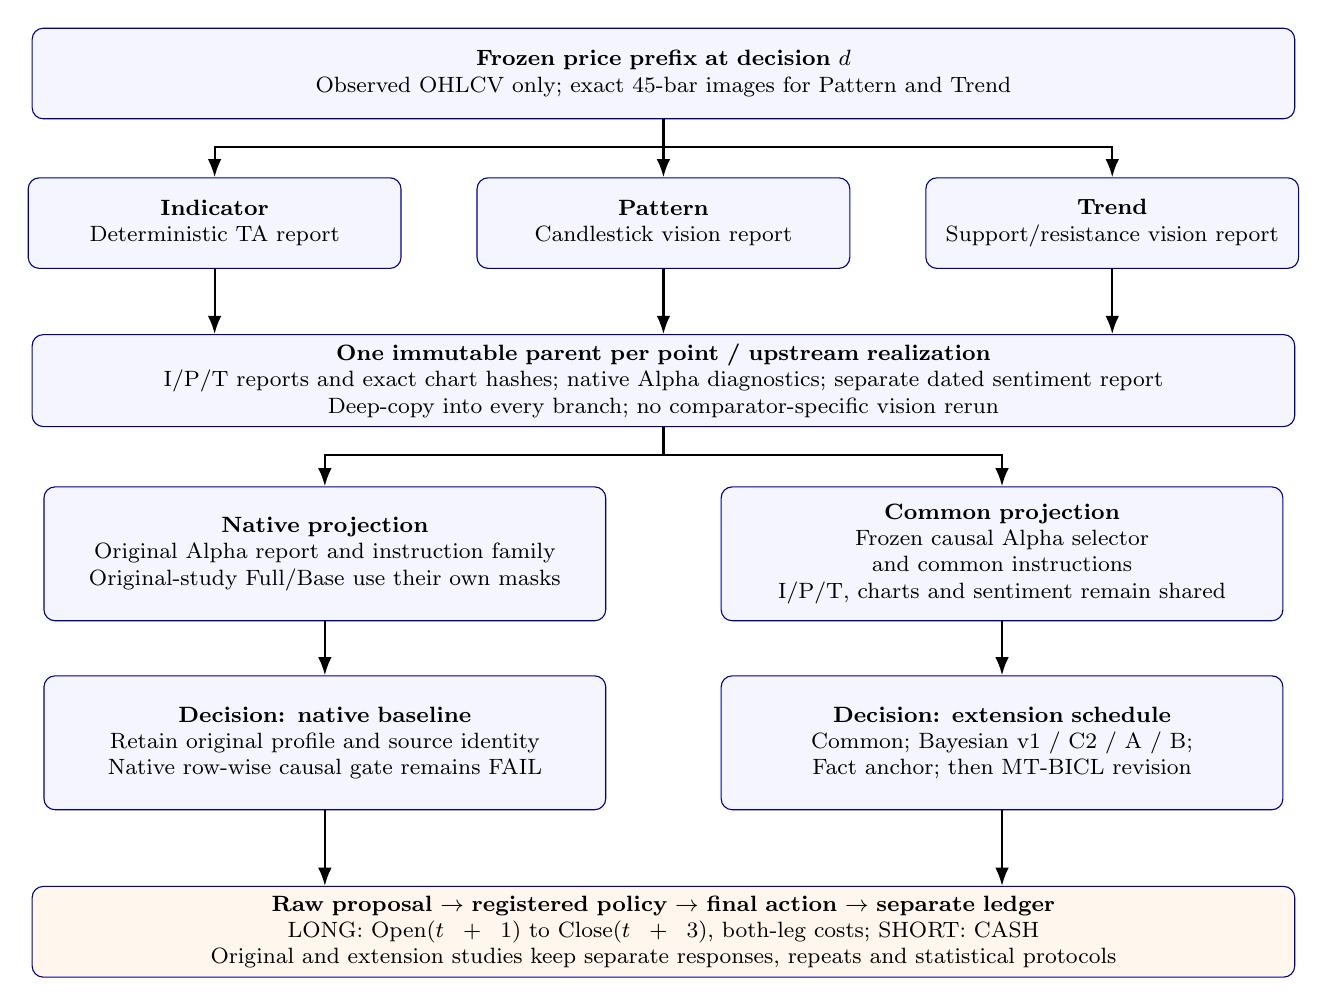
\begin{tikzpicture}[>=Latex,
 box/.style={draw=blue!55!black,fill=blue!4,rounded corners,align=center,text width=4.5cm,minimum height=1.15cm,font=\footnotesize},
 wide/.style={box,text width=15.8cm},half/.style={box,text width=6.9cm,minimum height=1.7cm},arr/.style={->,thick}]
\node[wide] (price) at (5.7,0) {\textbf{Frozen price prefix at decision $d$}\\Observed OHLCV only; exact 45-bar images for Pattern and Trend};
\node[box] (ind) at (0,-1.9) {\textbf{Indicator}\\Deterministic TA report};
\node[box] (pat) at (5.7,-1.9) {\textbf{Pattern}\\Candlestick vision report};
\node[box] (trend) at (11.4,-1.9) {\textbf{Trend}\\Support/resistance vision report};
\draw[arr] (price.south)--(pat.north);
\draw[arr] (price.south)--++(0,-0.35)-|(ind.north);
\draw[arr] (price.south)--++(0,-0.35)-|(trend.north);
\node[wide] (shared) at (5.7,-3.9) {\textbf{One immutable parent per point / upstream realization}\\I/P/T reports and exact chart hashes; native Alpha diagnostics; separate dated sentiment report\\Deep-copy into every branch; no comparator-specific vision rerun};
\foreach \n in {ind,pat,trend}{\draw[arr] (\n.south)--(\n.south |- shared.north);}
\node[half] (native) at (1.4,-6.1) {\textbf{Native projection}\\Original Alpha report and instruction family\\Original-study Full/Base use their own masks};
\node[half] (common) at (10,-6.1) {\textbf{Common projection}\\Frozen causal Alpha selector\\and common instructions\\I/P/T, charts and sentiment remain shared};
\draw[arr] (shared.south)--++(0,-0.35)-|(native.north);
\draw[arr] (shared.south)--++(0,-0.35)-|(common.north);
\node[half] (dn) at (1.4,-8.5) {\textbf{Decision: native baseline}\\Retain original profile and source identity\\Native row-wise causal gate remains FAIL};
\node[half] (dc) at (10,-8.5) {\textbf{Decision: extension schedule}\\Common; Bayesian v1 / C2 / A / B;\\Fact anchor; then MT-BICL revision};
\draw[arr] (native)--(dn);\draw[arr] (common)--(dc);
\node[wide,fill=orange!7] (out) at (5.7,-10.9) {\textbf{Raw proposal $\rightarrow$ registered policy $\rightarrow$ final action $\rightarrow$ separate ledger}\\LONG: Open$(t+1)$ to Close$(t+3)$, both-leg costs; SHORT: CASH\\Original and extension studies keep separate responses, repeats and statistical protocols};
\draw[arr] (dn.south)--(dn.south |- out.north);
\draw[arr] (dc.south)--(dc.south |- out.north);
\end{tikzpicture}

\caption{Shared-input system pipeline and the two alpha/prompt projections. Arrows show data flow; Indicator, Pattern and Trend execute once in sequence per upstream realization. The extension reuses their immutable parent across roles and three Decision repeats. Original Full/Base results use a separate response collection and their own masks. Decision dependencies and external action policy are detailed in Figure~\ref{fig:decision_agent}; neither projection certifies the whole system as causal.}
\label{fig:flow}
\end{figure}

\subsection{Indicator Agent}
Indicator Agent computes and renders five deterministic TA-Lib-based votes: MACD(12,26,9), RSI(14), Stochastic(14,3,3), Williams \%R(14) and ROC(10). They are momentum/trend indicators, not five volatility oscillators. Its backtest node returns a report and messages, without calling an LLM or forwarding the declared state schema's complete numeric arrays. Bollinger variables can be computed on the alpha path; BB/ADX state declarations do not create two additional Indicator votes. \ref{app:indicator_logic} specifies the ordered boundaries and missing-data convention \cite{talib_rsi_docs,talib_willr_docs}.

Four-decimal rounding precedes classification, nonfinite samples are removed and zero is retained. Crossovers take priority where specified; overlapping RSI/Williams thresholds require ordered branches rather than two simultaneous unconditional rules. Each missing/error result contributes a neutral vote within the fixed denominator of five. Directional plurality and the confidence categories are deterministic summary heuristics. They are not calibrated probabilities, and an immutable signal tally does not make a downstream narrative correct.

\subsection{Alpha Agent}
\paragraph{Alpha selection}
The Alpha role evaluates 85 native candidates: 80 retained WorldQuant adaptations and five custom formulas. It supplies a selected top-five report from the trailing prefix, using the diagnostic score in Eq.~\ref{eq:composite}. The transformations, metric support, IC orientation and native row-wise causal failure are defined in Section~\ref{sec:formulation}. A rolling own-history rank is not a cross-sectional rank, and the 21 exclusions are not all justified by an inability to translate cross-sectional operators. Full expressions and exception handling remain in the registry; \ref{app:signals} gives the custom formulas needed to read the reports.

Selection, IC sign and candidate diagnostics reuse trailing observations. Hence the current value is an input to a report, while the reported skill fields are in-sample ranking statistics. Neither choosing the top five nor reversing negative IC establishes out-of-sample profitability. Six selected metadata slots have description/handler mismatches; actual prompts, metadata and implementation identity are kept distinct. No historical prediction is repaired to agree with a corrected description.

\paragraph{Common projection and shared parent}
The extension binds a frozen selector to the same point, price prefix and native snapshot hash. Only the alpha report/factor fields are replaced for common-profile consumers; Indicator, Pattern, Trend, chart inputs and sentiment remain shared. Selector fits precede the test scope and are not repeated on a Decision repeat. Native is preserved for comparison rather than silently upgraded. The bridge therefore controls upstream realization while deliberately changing alpha representation and instruction family.

\paragraph{Sentiment integration}
Vietnamese sentiment is a separate contextual report, not an input to the native OHLCV factor formulas or score. The frozen provider supplies aggregate/count information and empty article-detail/peer lists. Relative sentiment and z-score fields on that path are consequently zero-valued outputs of the normalizer, rather than measured contemporaneous peer evidence. The three-article availability rule differs from the eight-article reliability flag. The 90-day window, 30-day decay, scorer revision and provenance limitations are specified in Section~\ref{sec:formulation}.

Figure~\ref{fig:alpha_agent} separates native selection, the frozen causal-common alpha projection and sentiment-context construction. Optional live endpoints, lexicon fallbacks and peer discovery are repository capabilities; they are not evidence that the corresponding inputs were used or historically available in the evaluated calls.

\begin{figure}[!htbp]
\centering% Hai profile alpha tách biệt; sentiment không đi vào công thức factor.
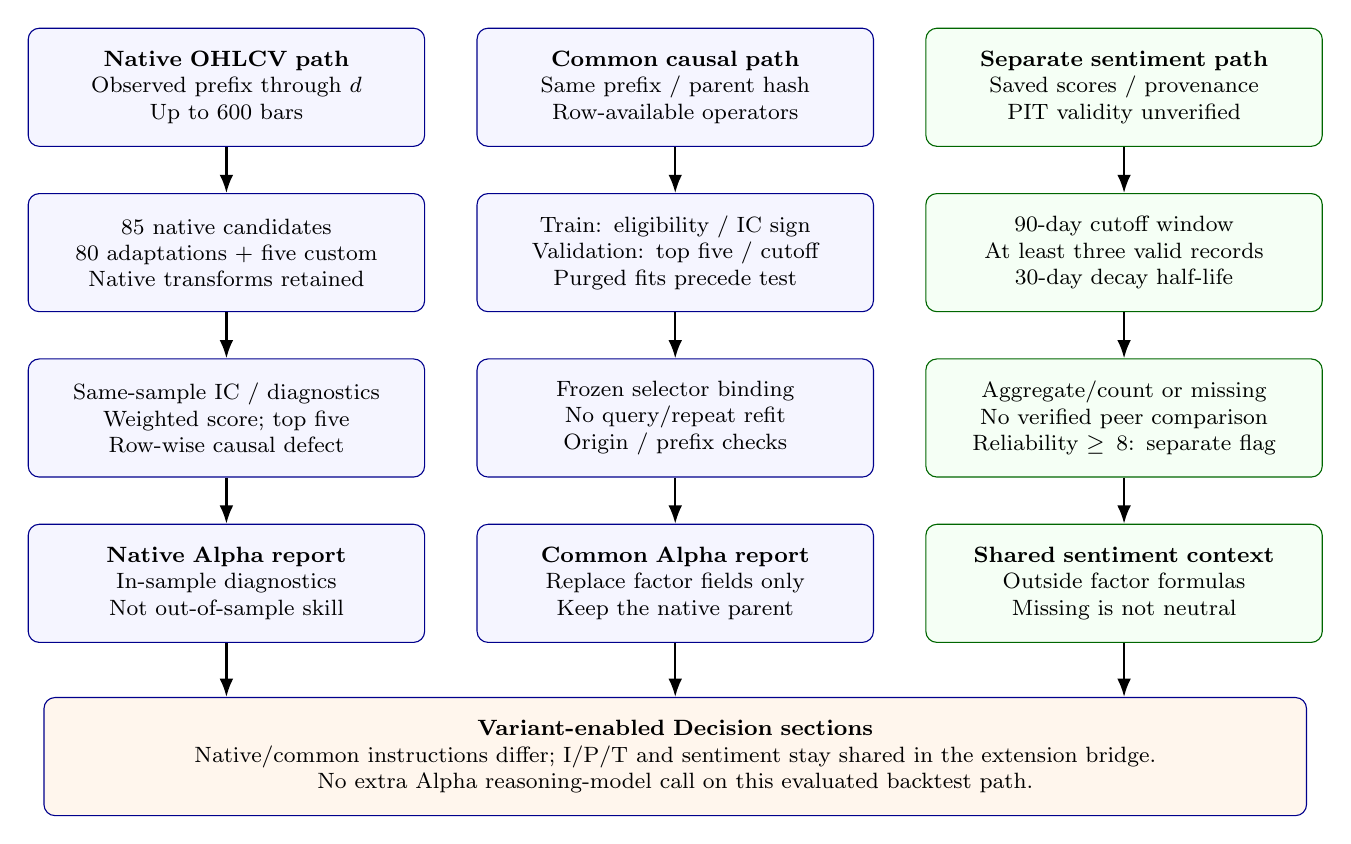
\begin{tikzpicture}[>=Latex,
 box/.style={draw=blue!55!black,fill=blue!4,rounded corners,align=center,text width=4.8cm,minimum height=1.5cm,font=\footnotesize},
 sent/.style={box,draw=green!40!black,fill=green!4},arr/.style={->,thick}]
\node[box] (n1) at (0,0) {\textbf{Native OHLCV path}\\Observed prefix through $d$\\Up to 600 bars};
\node[box] (c1) at (5.7,0) {\textbf{Common causal path}\\Same prefix / parent hash\\Row-available operators};
\node[sent] (s1) at (11.4,0) {\textbf{Separate sentiment path}\\Saved scores / provenance\\PIT validity unverified};
\node[box] (n2) at (0,-2.1) {85 native candidates\\80 adaptations + five custom\\Native transforms retained};
\node[box] (c2) at (5.7,-2.1) {Train: eligibility / IC sign\\Validation: top five / cutoff\\Purged fits precede test};
\node[sent] (s2) at (11.4,-2.1) {90-day cutoff window\\At least three valid records\\30-day decay half-life};
\node[box] (n3) at (0,-4.2) {Same-sample IC / diagnostics\\Weighted score; top five\\Row-wise causal defect};
\node[box] (c3) at (5.7,-4.2) {Frozen selector binding\\No query/repeat refit\\Origin / prefix checks};
\node[sent] (s3) at (11.4,-4.2) {Aggregate/count or missing\\No verified peer comparison\\Reliability $\ge8$: separate flag};
\node[box] (n4) at (0,-6.3) {\textbf{Native Alpha report}\\In-sample diagnostics\\Not out-of-sample skill};
\node[box] (c4) at (5.7,-6.3) {\textbf{Common Alpha report}\\Replace factor fields only\\Keep the native parent};
\node[sent] (s4) at (11.4,-6.3) {\textbf{Shared sentiment context}\\Outside factor formulas\\Missing is not neutral};
\foreach \a/\b in {n1/n2,n2/n3,n3/n4,c1/c2,c2/c3,c3/c4,s1/s2,s2/s3,s3/s4}{\draw[arr] (\a)--(\b);}
\node[box,text width=15.8cm,fill=orange!7] (out) at (5.7,-8.5) {\textbf{Variant-enabled Decision sections}\\Native/common instructions differ; I/P/T and sentiment stay shared in the extension bridge.\\No extra Alpha reasoning-model call on this evaluated backtest path.};
\foreach \n in {n4,c4,s4}{\draw[arr] (\n.south)--(\n.south |- out.north);}
\end{tikzpicture}

\caption{Alpha Agent profiles and separate sentiment context. The native path retains its in-sample ranking and row-wise causal defects. The common projection uses row-available operators and a selector fixed by chronological training/purged validation. Sentiment enters the enabled Decision text separately; it is not a factor-score input or authenticated peer comparison. Freezing the common selector does not repair the native profile.}
\label{fig:alpha_agent}
\end{figure}

\subsection{Pattern Agent}
Pattern Agent analyses a candlestick PNG rendered from the exact 45-bar window. The prompt requests a chart formation, recent-candle evidence, directional bias, confidence and trading implication. The report parser retains the structured text fields; format completion and consistency checks are distinguished from financial correctness. Figure~\ref{fig:charts} presents an actual archived chart pair rather than a synthetic demonstration.

Candle bodies are green when Close exceeds Open and red otherwise, including a doji. This is an Open--Close body rule, not the Vietnamese exchange board's reference-price colouring rule. The exchange-board convention is not used to infer candle direction. After inference, consistency rules compare the claimed bias with simple OHLCV-derived properties such as the final body and recent closes. A contradiction flag can reduce displayed confidence; it cannot reveal which candle the VLM actually attended to. Alternative text-only paths in the general application are not assumed to have replaced any frozen vision input.

\begin{figure}[!htbp]
\centering
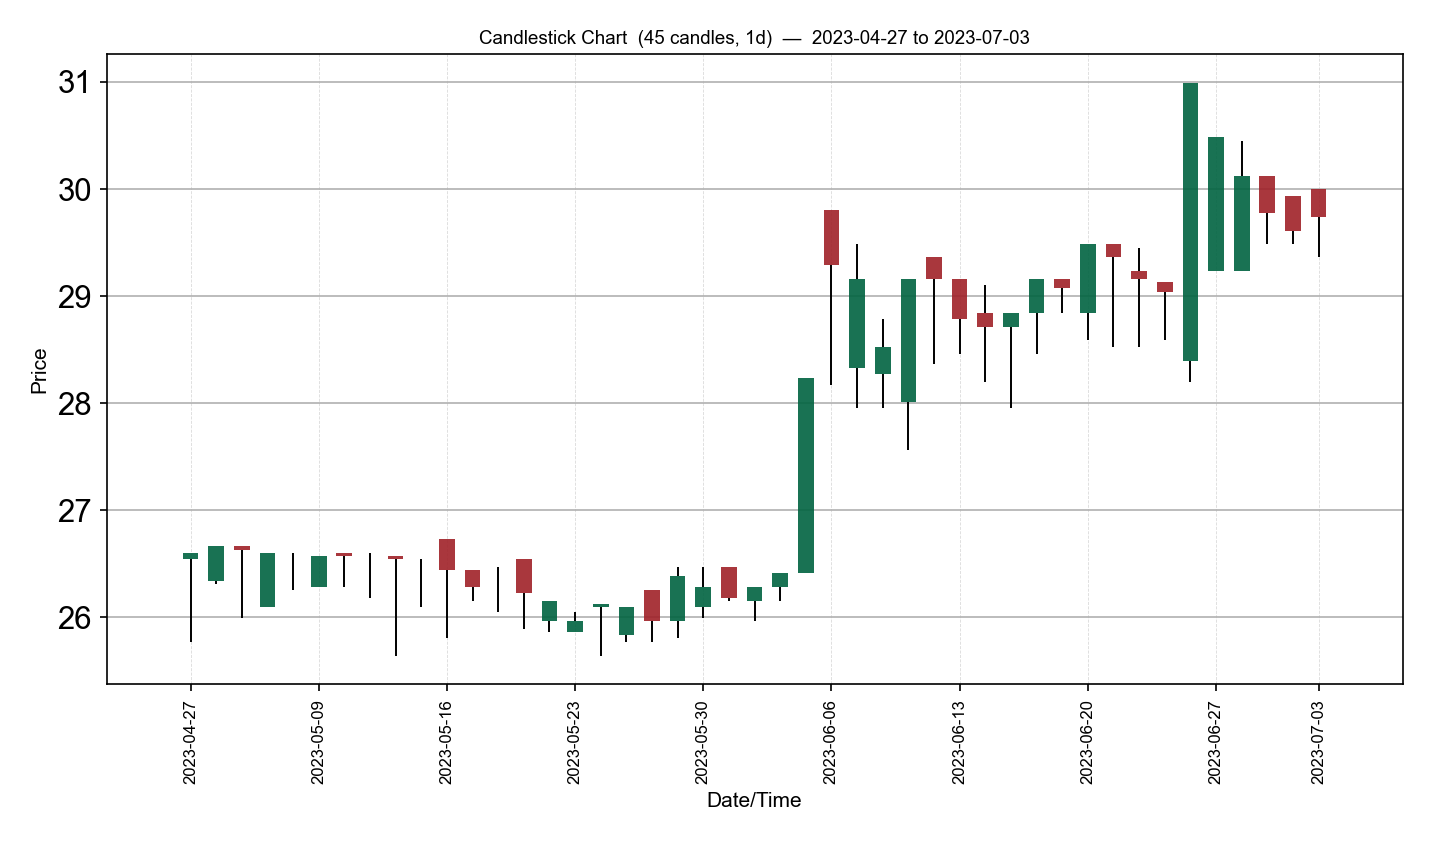
\includegraphics[width=0.90\textwidth]{figs/final_pattern.png}\par\smallskip
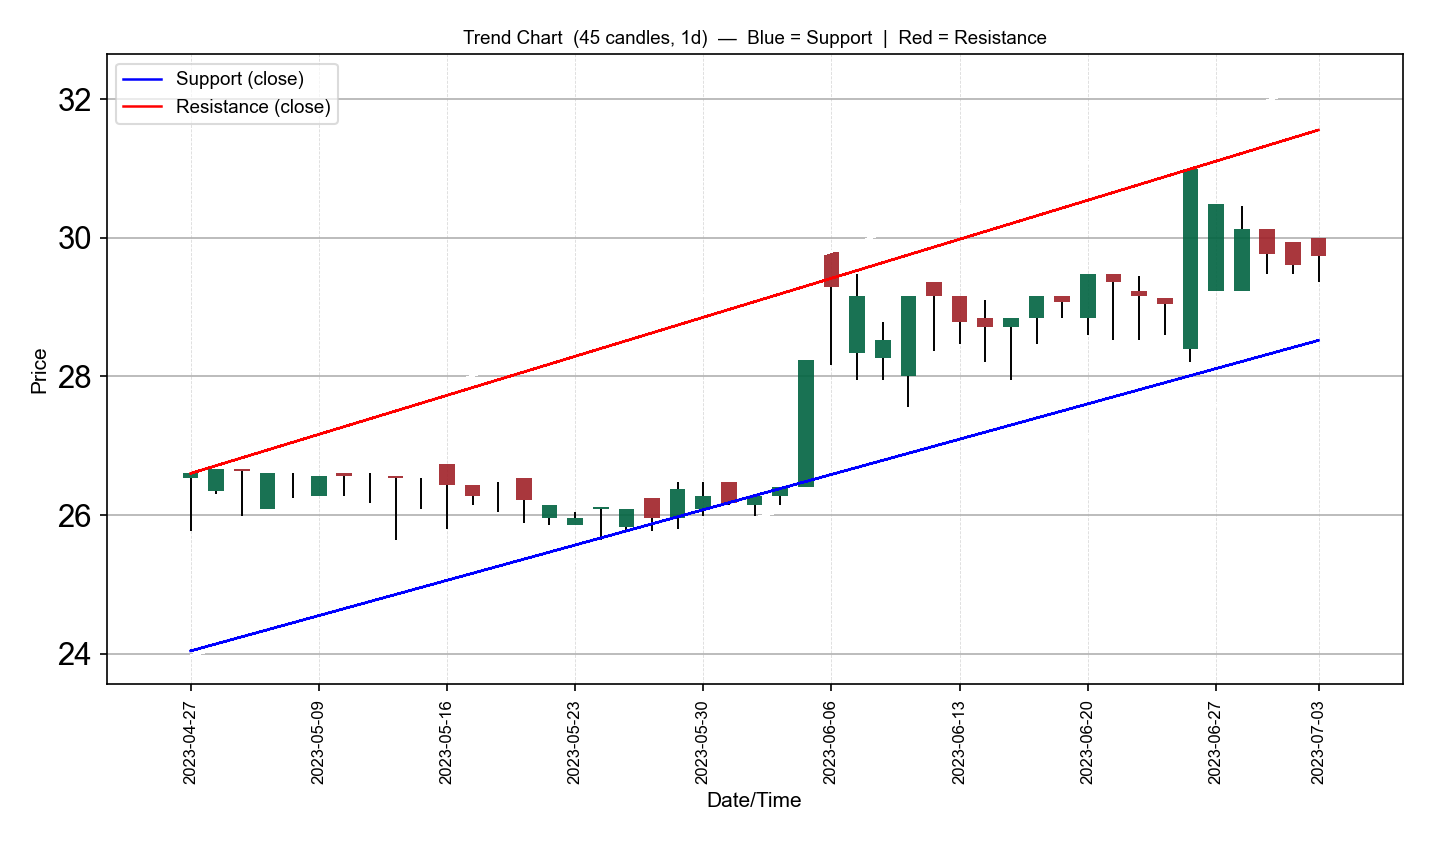
\includegraphics[width=0.90\textwidth]{figs/final_trend.png}
\caption{Actual Pattern and corrected Trend inputs for CMG on 3 July 2023, the first chronologically eligible main unit. Bodies compare Close with Open; the Trend legend maps blue to support and red to resistance. The unit was selected by date then symbol/ID without inspecting outcomes.}
\label{fig:charts}
\end{figure}

\subsection{Trend Agent}
Trend Agent receives a separate chart with fitted support/resistance lines. The inherited fitting utility starts with a least-squares close-price line, selects upper/lower deviation pivots, and optimizes a slope through each pivot under a non-crossing constraint. It implements both a close-only channel and a high/low channel, the latter using close-price regression to find pivots and high/low data for the bounds. These are numerical lines over the supplied window, not human-verified latent support levels.

For row position $u$, a fitted line has form $b+mu$. A support bound must remain below the corresponding price sequence within the implementation tolerance; resistance must remain above it. The local slope search reduces its step when the squared-deviation objective fails to improve or violates the constraint. The VLM then describes direction, levels, slope, price relative to support, forecast and confidence. Support is drawn blue and resistance red. A deterministic consistency check against simple price/trend summaries does not validate every reported level or coordinate.

The renderer audit matched 204 images across 102 units byte for byte and pixel for pixel, and 240 actual vision requests matched their image caches and Vietnamese templates. It verified body geometry, colour and legend handles, not the model's visual understanding. In particular, the Vietnamese word \emph{xanh} is less colour-specific than the corrected English ``blue'' wording. Inherited high-frequency/K-line prompt language also remains distinguishable from this daily-bar application. Matched local-pattern interventions and trend swaps would be needed to test whether the model uses the purported visual evidence.

\subsection{Decision Agent}
Decision receives condensed Indicator, Pattern and Trend reports plus enabled factor/sentiment sections. Reports are distilled and capped before prompt composition. The original study's observed successful Decision prompts are at most 4,187 characters, below the 6,500-character guard. Figure~\ref{fig:decision_agent} shows the extension dependencies, raw proposals, fallback and separate action policy.

\begin{figure}[!htbp]
\centering% Mũi tên giữa vai trò là dependency cùng repeat; policy tách raw/final.
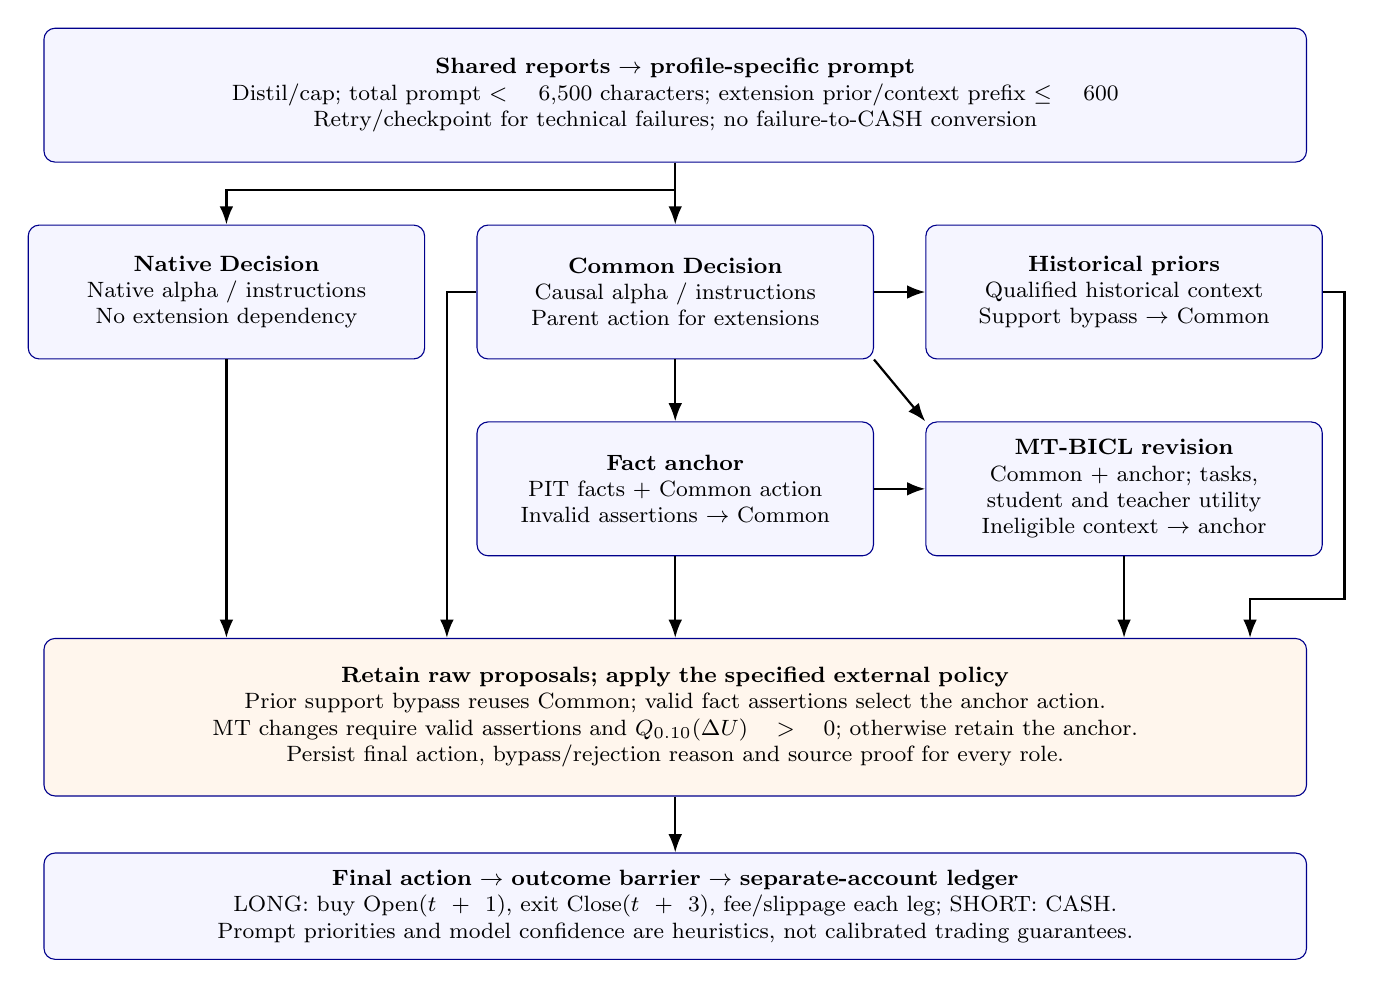
\begin{tikzpicture}[>=Latex,
 box/.style={draw=blue!55!black,fill=blue!4,rounded corners,align=center,text width=4.8cm,minimum height=1.7cm,font=\footnotesize},
 wide/.style={box,text width=15.8cm},arr/.style={->,thick}]
\node[wide] (in) at (5.7,0) {\textbf{Shared reports $\rightarrow$ profile-specific prompt}\\Distil/cap; total prompt $<6{,}500$ characters; extension prior/context prefix $\le600$\\Retry/checkpoint for technical failures; no failure-to-CASH conversion};
\node[box] (native) at (0,-2.5) {\textbf{Native Decision}\\Native alpha / instructions\\No extension dependency};
\node[box] (common) at (5.7,-2.5) {\textbf{Common Decision}\\Causal alpha / instructions\\Parent action for extensions};
\node[box] (prior) at (11.4,-2.5) {\textbf{Historical priors}\\Qualified historical context\\Support bypass $\rightarrow$ Common};
\draw[arr] (in.south)--++(0,-0.35)-|(native.north);
\draw[arr] (in.south)--(common.north);
\draw[arr] (common.east)--(prior.west);
\node[box] (fact) at (5.7,-5) {\textbf{Fact anchor}\\PIT facts + Common action\\Invalid assertions $\rightarrow$ Common};
\node[box] (mt) at (11.4,-5) {\textbf{MT-BICL revision}\\Common + anchor; tasks,\\student and teacher utility\\Ineligible context $\rightarrow$ anchor};
\draw[arr] (common.south)--(fact.north);
\draw[arr] (common.south east)--(mt.north west);
\draw[arr] (fact.east)--(mt.west);
\node[wide,fill=orange!7,minimum height=2cm] (policy) at (5.7,-7.9) {\textbf{Retain raw proposals; apply the specified external policy}\\Prior support bypass reuses Common; valid fact assertions select the anchor action.\\MT changes require valid assertions and $Q_{0.10}(\Delta U)>0$; otherwise retain the anchor.\\Persist final action, bypass/rejection reason and source proof for every role.};
\draw[arr] (native.south)--(native.south |- policy.north);
\draw[arr] (common.west)--(2.8,-2.5)--(2.8,-6.8)--(2.8,-6.8 |- policy.north);
\draw[arr] (prior.east)--(14.2,-2.5)--(14.2,-6.4)--(13,-6.4)--(13,-6.4 |- policy.north);
\draw[arr] (fact.south)--(fact.south |- policy.north);
\draw[arr] (mt.south)--(mt.south |- policy.north);
\node[wide,minimum height=1.35cm] (ledger) at (5.7,-10.3) {\textbf{Final action $\rightarrow$ outcome barrier $\rightarrow$ separate-account ledger}\\LONG: buy Open$(t+1)$, exit Close$(t+3)$, fee/slippage each leg; SHORT: CASH.\\Prompt priorities and model confidence are heuristics, not calibrated trading guarantees.};
\draw[arr] (policy)--(ledger);
\end{tikzpicture}

\caption{Decision dependencies and raw-to-final action policy. Role-to-role arrows require the completed record from the same repeat; the four prior methods are parallel dependants of Common. Support bypass reuses a parent without an LLM call. Fact assertions and the MT utility veto are external policies, not model reasoning guarantees. Raw/final actions and rejection/bypass proofs remain distinct; technical failures use retry/checkpoint handling.}
\label{fig:decision_agent}
\end{figure}

The instructions ask for trend/key-level assessment, recent-candle evidence, momentum confirmation and comparison with enabled factor/sentiment context. Price/chart evidence has priority, quantitative factors may challenge it, and sentiment has lower priority. These instructions describe an intended analysis sequence; they are not an independently observed internal reasoning trace or a guaranteed conflict-resolution algorithm.

The required output includes a binary LONG/SHORT forecast, forecast horizon, confidence, risk/reward field, evidence for/against and justification. Model confidence and risk/reward statements do not constitute calibrated uncertainty or executable price levels. In the long-only reference ledger, SHORT maps to CASH and LONG to the specified next-open/target-close cycle. The classifier's labels and account execution remain distinct.

Base retains the same upstream content and general instructions but removes both alpha and sentiment sections; those concepts may still appear in general instructions. Thus Full--Base changes a bundle and prompt length, not solely one numerical factor. Main/upstream prompts use compact factor text, whereas factorial A/AS/P deliver five explicit rows. The resulting representation difference remains part of the interpretation of the separate panels.

\paragraph{Historical-prior methods}
Bayesian v1 retrieves up to three matured same-symbol examples using regime and report-signal context, and appends a compact historical prior. C2 adds conditional Beta-based statistics on matched Trend/Pattern/Alpha/Indicator states, shrinkage using a disjoint background and independent readiness gates for statistics and examples. A\_tp\_pool relaxes the conditioning match to Trend/Pattern to increase usable conditional support. B\_semantic retains C2's evidence/readiness but makes the meaning of its historical counts, intervals and example identifiers more explicit; it is not a separately trained semantic embedding retriever. Historical rates and plug-in credible intervals are not query probabilities or expected returns. If no qualified prior block is visible, the method reuses the same repeat's Common action and records the reason; it does not issue a duplicate Decision call.

\paragraph{Fact anchor and MT-BICL}
Fact\_Anchor receives a deterministic point-in-time fact packet, including MACD-versus-signal and Close-versus-SMA20 assertions, and the completed Common decision. Valid assertions select its proposed action without the numerical utility veto; invalid assertions select Common with a source proof. MT-BICL constructs numerical prior/target tasks conditioned on the factual bucket, retains a frozen student estimate and teacher-based utility summary, and requests a revision of that anchor only when context is eligible. The external policy in Eq.~\ref{eq:revision_utility} decides whether a changed proposal is accepted. Raw proposals, anchor actions, bypass and final actions are distinct saved fields, so final outcome differences cannot be assigned entirely to the LLM or student.

All extension prompts preserve report distillation/capping, require fewer than 6,500 characters and cap their prior/context prefix at 600 characters. The original-study maximum of 4,187 characters above is not an extension-run maximum. Exact prompt projections, readiness thresholds and request schemas are given in \ref{app:prompts} and~\ref{app:state_schema}; runtime resources and restore instructions are in \ref{app:software}.
\FloatBarrier

\section{Experimental Setup}
\label{sec:experimentalsetup}

\subsection{Dataset and Point-in-Time Data Contract}
The daily universe spans information technology (FPT, CMG), banking (VCB, MBB), retail (MWG), food/beverages (VNM, BHN) and aviation/tourism (HVN, VJC). This is a purposive, non-representative sample: BHN, CMG, FPT, HVN, MBB, MWG, VCB, VJC and VNM. The reconstructed vnstock/VCI price snapshot \cite{vnstock_docs} covers observed vendor sessions from 2020 through September 2026. It is not an authenticated submission-time snapshot. Contradictory BHN OHLC data trigger the frozen valid-suffix policy; insufficient subsequent warm-up excludes BHN from three early blocks. No price is corrected to improve a result. This leaves 102 eligible cells of the 12-date by nine-symbol grid in Figure~\ref{fig:calendar}.

\paragraph{Two study identities}
We distinguish the original Full/Base revision study from the extension collection U08 and its frozen U09 analysis (editorial ID \texttt{unified\_u08\_u09\_r1}). They use the same eligible market calendar, but separate responses, method interfaces and provenance. Original-study Base omits both factor and sentiment sections; Common in the extension retains them under a different alpha/prompt profile. No original prediction is replaced by an extension prediction, and matching calendars do not justify a cross-study paired contrast or summed sample size. Sentiment is unavailable at \UnifiedMissingSentiment/\UnifiedPoints\ extension points; this remains missing input, not observed neutral sentiment.

\subsection{Walk-Forward Protocol}
Six blocks cover 2023 H2, 2024 H2, 2025 H1, 2025 Q4, 2026 Q2 and 2026 Q3, with two scheduled dates per block. These are twelve selected dates, not a continuous multi-year daily backtest; the chronological evaluation follows the walk-forward principle \cite{pardo2008evaluation} under this explicitly reduced schedule. Cross-symbol observations share calendar shocks. The 51 eligible symbol--block scopes contain chronological train/validation/test partitions: every train label exits before validation starts, and every validation label exits before the first test decision. Cutoffs require the frozen history length; label spans touching the next partition are purged.

The reduced scope was amended after some inference to complete a bounded historical study. Its 375 registered Decisions include 193 explicitly reused successful executions and 182 further successes. The factorial subset was selected by metadata (symbol/date round-robin), not prediction quality, but this does not make the overall amendment preregistered. The larger legacy grids remain incomplete/superseded. Table~\ref{tab:scope} distinguishes shared r0 calls, additional realizations and the separate factorial panel; their observations are not summed as independent markets.

\begin{figure}[!htb]
\centering
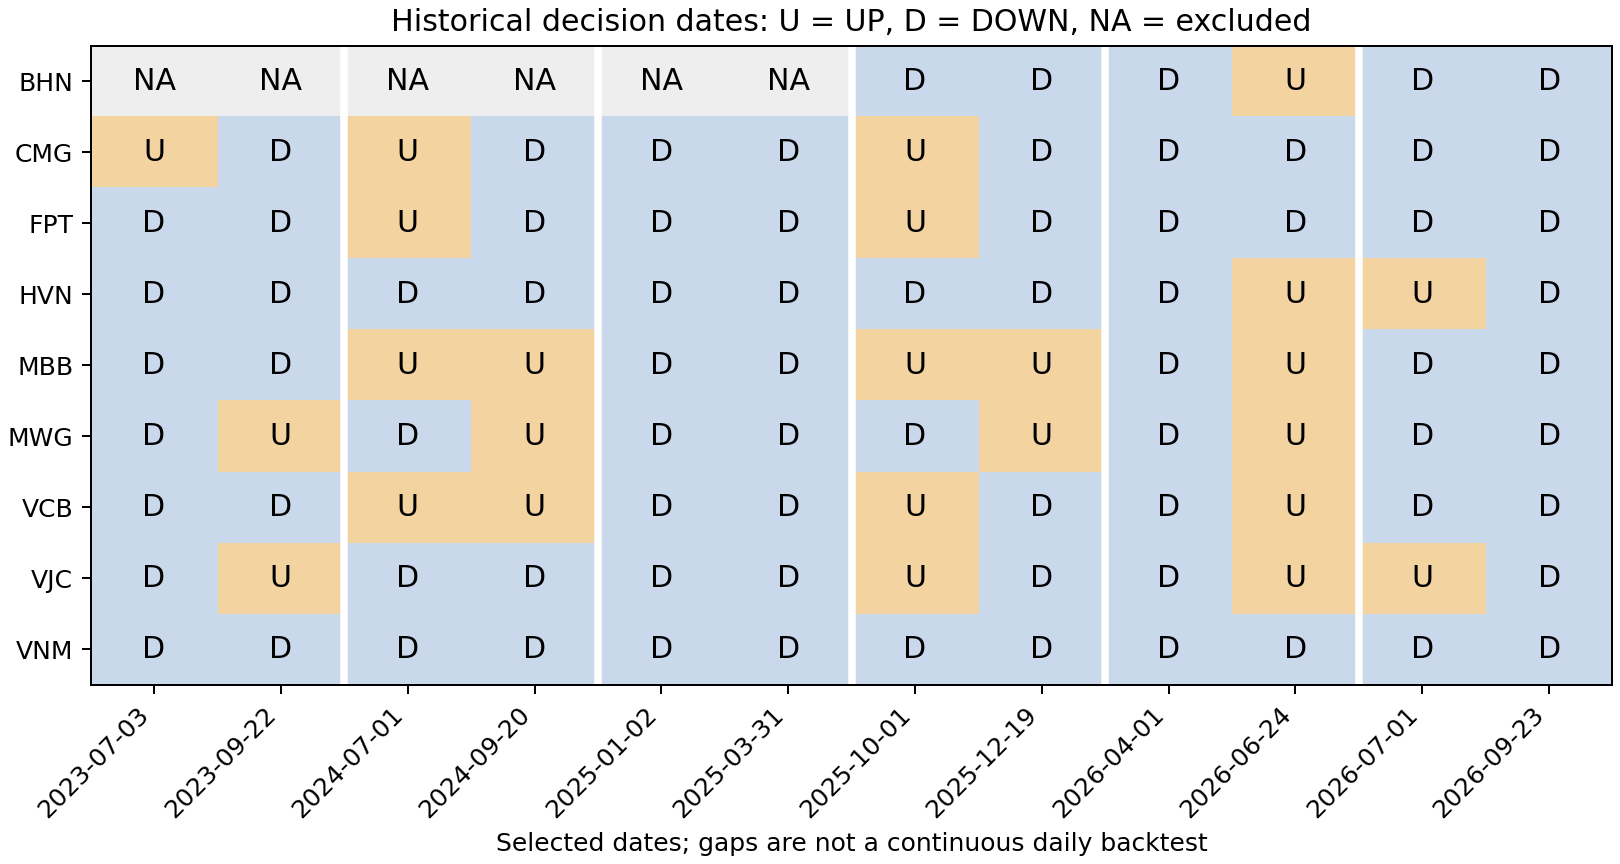
\includegraphics[width=\textwidth]{figs/final_calendar.png}
\caption{Historical decision dates and eligibility shared by the original and extension studies. Matching dates do not imply shared inference responses. Missing BHN cells remain excluded rather than being filled with CASH predictions. Labels are shared evaluation truth, not a visualization selected from Full's successful forecasts.}
\label{fig:calendar}
\end{figure}
\begin{table}[!htb]
\centering\small
\setlength{\tabcolsep}{3pt}
\renewcommand{\arraystretch}{1.15}
\caption{Evaluation scopes and prompt variants in the frozen historical study. Shared main/upstream executions are counted once.}
\label{tab:scope}
\textbf{A. Recorded supports}\par\smallskip
\begin{tabular}{lrrrrrrr}
\hline
Scope & $N$/exec. & Symbols & Dates & Blocks & UP/DOWN & Exec. & Decisions \\
\hline
Main & 102 & 9 & 12 & 6 & 25/77 & 1 & 204 \\
Upstream & 9 & 9 & 3 & 3 & 2/7 & 3 & 54 \\
Factorial & 9 & 8 & 4 & 3 & 2/7 & 3 & 135 \\
\hline
\end{tabular}\par\medskip
\textbf{B. Prompt sections}\par\smallskip
\begin{tabular}{llll}
\hline
Variant & Factors & Sentiment & Representation \\
\hline
B & -- & -- & Shared price reports \\
A & Current & -- & Five-row factorial \\
S & -- & Current & Factorial \\
AS & Current & Current & Compact main / five-row factorial \\
P & Past donor & Current & Five-row factorial \\
\hline
\end{tabular}\par\medskip
\begin{minipage}{\textwidth}\footnotesize Main uses B/AS; upstream uses B/AS; factorial uses B/A/S/AS/P. Class counts are per execution. Upstream includes 18 main r0 calls: 204+54+135-18=375 unique Decisions. P preserves current names/schema/missingness and sentiment, replacing factor values/signals/skill metadata by one past train-only rank-vector donor.\end{minipage}
\end{table}


The extension fixes \UnifiedPoints\ points, \UnifiedAccounts\ symbol--fold accounts, \UnifiedUpstreamRealizations\ upstream realization per point and \UnifiedDecisionRepeats\ Decision repeats. One immutable report/image parent is deep-copied into all roles; each repeat uses new Decision responses where a call is eligible. The \UnifiedForecastSlots\ research slots are not independent market samples, full-system executions or successful HTTP calls. All 102 evaluation IDs are reserved globally before context labels can be computed, including IDs belonging to earlier folds. Context is frozen before the first test query in a fold and reused at its second anchor; test labels are never added prequentially.
\begingroup
\let\savedscopepresentationtable\table
\def\table[#1]{\savedscopepresentationtable[!htbp]}
\begin{table}[!htb]
\centering\small
\setlength{\tabcolsep}{3pt}
\renewcommand{\arraystretch}{1.12}
\caption{Extension study U08/U09: distinct support and execution counts.}
\label{tab:u09-scope}
\textbf{Recorded support}\par\smallskip
\begin{tabular}{lr}
\hline
Quantity & Count \\
\hline
Market points & 102 \\
Symbols & 9 \\
Dates & 12 \\
Folds & 6 \\
Independent-capital accounts per repeat & 51 \\
Upstream realizations per point & 1 \\
Upstream executions & 102 \\
Points without available sentiment & 79 \\
Decision repeats & 3 \\
Research forecast slots (eight roles) & 2448 \\
Raw Decision responses & 1290 \\
HTTP attempts (including retired) & 1702 \\
\hline
\end{tabular}\par\medskip
\begin{minipage}{\textwidth}\footnotesize This study shares a test calendar with the original study, not its responses. Three Decision repeats do not add market observations or upstream realizations. BHN contributes six points in three recent folds; the other eight symbols contribute twelve each. Unavailable sentiment is missing input, not neutral news.\end{minipage}
\end{table}

\endgroup
% Không để bảng phạm vi trôi sang phần Results của bản submit.
\FloatBarrier

\begin{figure}[!htb]
\centering% Cutoff/context và hàng rào outcome; không đưa nhãn query vào prompt.
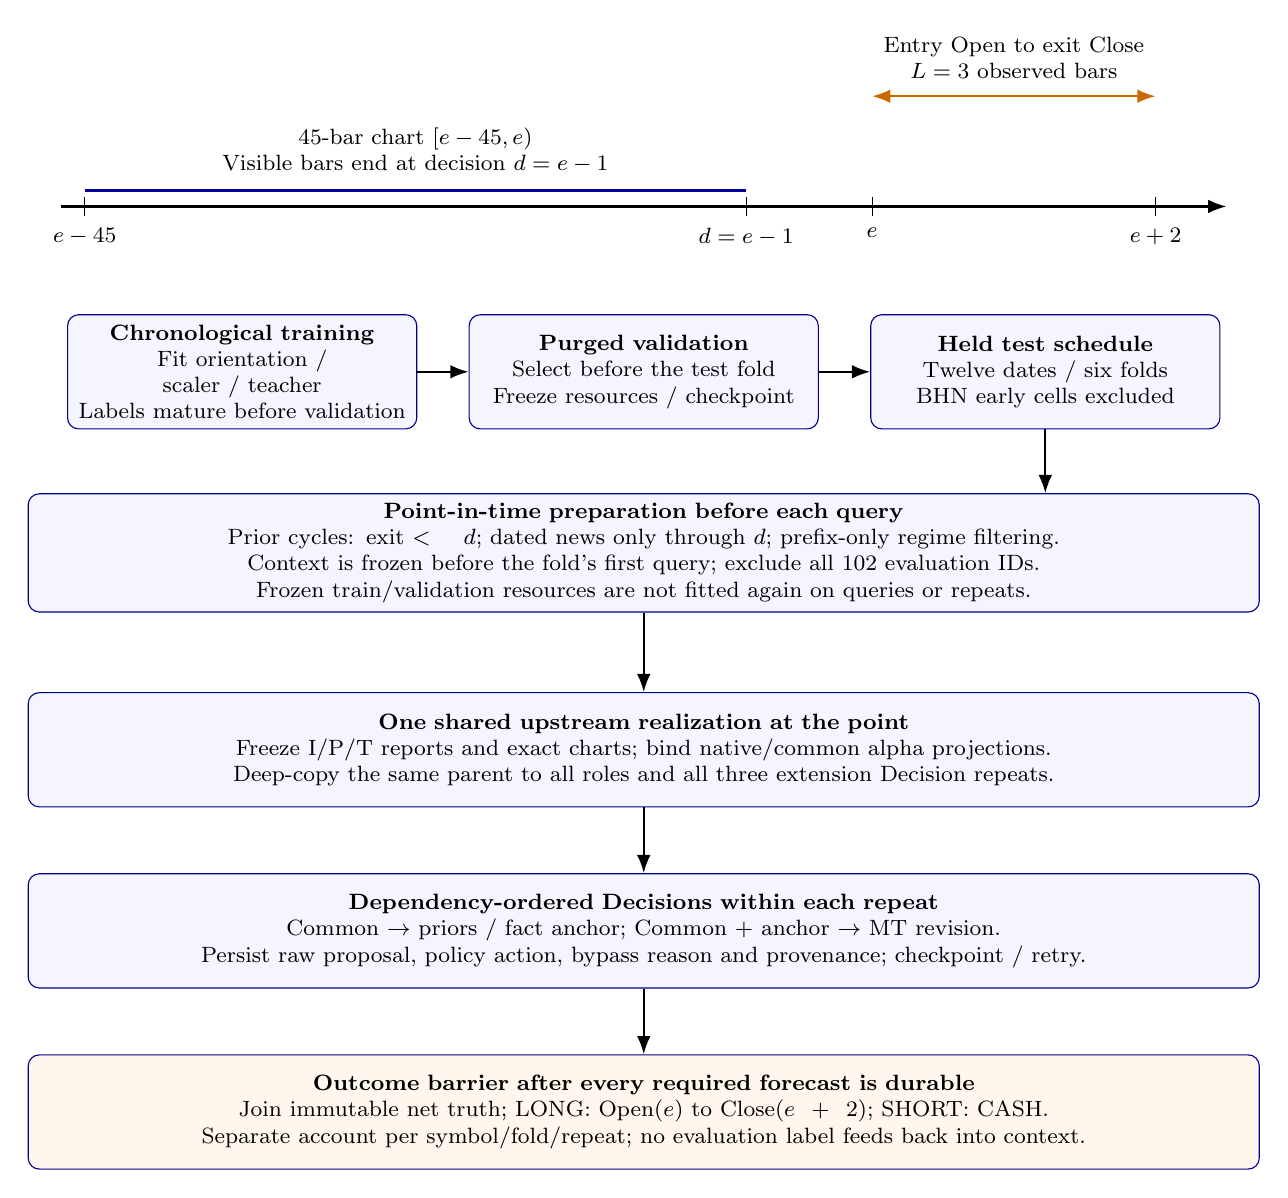
\begin{tikzpicture}[>=Latex,
 box/.style={draw=blue!55!black,fill=blue!4,rounded corners,align=center,text width=4.2cm,minimum height=1.45cm,font=\footnotesize},
 wide/.style={box,text width=15.4cm},arr/.style={->,thick}]
\draw[->,thick] (-0.3,0)--(14.5,0);
\draw[very thick,blue!60!black] (0,0.2)--(8.4,0.2);
\node[above,align=center,font=\footnotesize] at (4.2,0.3) {45-bar chart $[e-45,e)$\\Visible bars end at decision $d=e-1$};
\foreach \x/\lab in {0/{e-45},8.4/{d=e-1},10/{e},13.6/{e+2}}{\draw (\x,-0.12)--(\x,0.12);\node[below,font=\footnotesize] at (\x,-0.15) {$\lab$};}
\draw[<->,thick,orange!80!black] (10,1.4)--(13.6,1.4);
\node[above,align=center,font=\footnotesize] at (11.8,1.5) {Entry Open to exit Close\\$L=3$ observed bars};
\node[box] (train) at (2,-2.1) {\textbf{Chronological training}\\Fit orientation / scaler / teacher\\Labels mature before validation};
\node[box] (valid) at (7.1,-2.1) {\textbf{Purged validation}\\Select before the test fold\\Freeze resources / checkpoint};
\node[box] (test) at (12.2,-2.1) {\textbf{Held test schedule}\\Twelve dates / six folds\\BHN early cells excluded};
\draw[arr] (train)--(valid);\draw[arr] (valid)--(test);
\node[wide] (context) at (7.1,-4.4) {\textbf{Point-in-time preparation before each query}\\Prior cycles: exit $<d$; dated news only through $d$; prefix-only regime filtering.\\Context is frozen before the fold's first query; exclude all 102 evaluation IDs.\\Frozen train/validation resources are not fitted again on queries or repeats.};
\draw[arr] (test.south)--(test.south |- context.north);
\node[wide] (shared) at (7.1,-6.9) {\textbf{One shared upstream realization at the point}\\Freeze I/P/T reports and exact charts; bind native/common alpha projections.\\Deep-copy the same parent to all roles and all three extension Decision repeats.};
\draw[arr] (context)--(shared);
\node[wide] (decision) at (7.1,-9.2) {\textbf{Dependency-ordered Decisions within each repeat}\\Common $\rightarrow$ priors / fact anchor; Common + anchor $\rightarrow$ MT revision.\\Persist raw proposal, policy action, bypass reason and provenance; checkpoint / retry.};
\draw[arr] (shared)--(decision);
\node[wide,fill=orange!7] (out) at (7.1,-11.5) {\textbf{Outcome barrier after every required forecast is durable}\\Join immutable net truth; LONG: Open$(e)$ to Close$(e+2)$; SHORT: CASH.\\Separate account per symbol/fold/repeat; no evaluation label feeds back into context.};
\draw[arr] (decision)--(out);
\end{tikzpicture}

\caption{Walk-forward timing, frozen resources and forecast/outcome barrier. The chart ends at $d=e-1$, entry is at $e$ and the $L=3$ target is at $e+2$: equivalently Open$(t+1)$ to Close$(t+3)$. Prior exits precede the cutoff and all evaluation IDs stay outside context. The extension uses one upstream realization and three Decision repeats per point on twelve selected dates/six folds, not a uniform $S=3$ grid. Outer cutoff isolation does not certify native row-wise causality.}
\label{fig:walkforward}
\end{figure}

\subsection{Paired Baseline and Disentangled Ablations}
All nine classifiers use the same 102 main units and net target. CASH and always-LONG are constant predictions; always-LONG closes and pays costs every cycle. Train-majority uses purged training labels, choosing CASH on a tie. Momentum predicts LONG for a strictly positive trailing 20-session return. The logistic comparators use scikit-learn \cite{pedregosa2011sklearn}. Logistic-price uses numerical price features; logistic-matched adds the recorded factor/sentiment/missingness inputs. Imputation, scaling, regularization and decision threshold selection follow chronological train/validation rules; final logistic refits use matured train plus validation only. We reuse their saved predictions rather than refitting after observing outcomes. The fixed factor-vote comparator uses training-fitted medians/orientation and differs from the native top-five policy and the auxiliary numeric-control study.

Matched numerical inputs do not equal chart images, report wording or pretrained knowledge. Full--Base differences likewise include prompt structure, report length and propensity to choose CASH. The upstream panel has nine units, B/AS and three regenerated upstream realizations with a Decision execution per realization. The factorial panel has nine different-support units, B/A/S/AS/P and three Decision executions with fixed upstream. Both have two UP/seven DOWN per execution, but only the former covers nine symbols. We do not infer main-grid variability or separate upstream/Decision variance components from their SDs.

P retains current factor names, headings, schema/missingness and sentiment, replacing scalar values, signals and skill fields using a predetermined earlier train-only rank-vector donor. Donor label exits precede validation/test. Rank mapping is not name-matched covariance preservation, a placebo distribution or exposure matching. Five explicit rows reach each A/AS/P factorial prompt. Main/upstream compact prompts are a separate representation family. Interaction is defined as $AS-A-S+B$; the observed best-single gap $AS-\max(A,S)$ is a different, post-hoc diagnostic and not an eighth factorial contrast.

\paragraph{Extension baselines and dependencies}
The extension evaluates Native, Common, five extensions, Fact\_Anchor and two no-LLM controls, CASH and Always-LONG cycles with full costs. Five extensions are compared separately with Native (system family) and Common (method family). Fact\_Anchor is a dependency/control, not a sixth claimed improvement. Three descriptive bridges compare Common with Native, Fact\_Anchor with Common, and MT-BICL with Fact\_Anchor. Neither these bridges nor economic controls enter the primary contrast family. The original nine-unit upstream/factorial panels above remain evidence for their own interventions; new retrieval/content/MT ablations were not executed in U08/U09.

\subsection{Account and Statistical Metrics}
BA averages UP and DOWN recall \cite{brodersen2010balanced}; MCC \cite{chicco2020mcc} and both-class precision/recall accompany ordinary accuracy and LONG rate. Pooled metrics retain actual class supports. Symbol macro means are unweighted and report planned/defined denominators. Missing class support or a degenerate MCC denominator yields NA, not zero. Following dependent-data resampling principles \cite{lahiri2003resampling}, main contrasts use 10,000 paired whole-block resamples, seed 20261102, retaining dates, cross-section, variants and eligibility together. Repeat diagnostics jointly resample recorded blocks and paired execution indices. Intervals condition on finite draws; undefined counts remain visible. Circular block lengths, leave-one-block-out and Bartlett HAC \cite{newey1987hac} at lags 0/1/2 are sensitivity diagnostics. HAC uses calendar-aligned accuracy differences in fixed-universe panels, with a $t(n_{dates}-1)$ reference; few clusters, irregular gaps and post-inference additions prevent calibrated significance or power claims.

To specify the classification estimand, let TP/FN count UP outcomes and TN/FP count DOWN outcomes. We use
\begin{equation}
 \begin{aligned}
 BA&=\frac12\left(\frac{TP}{TP+FN}+\frac{TN}{TN+FP}\right),\\
 MCC&=\frac{TP\,TN-FP\,FN}{\sqrt{(TP+FP)(TP+FN)(TN+FP)(TN+FN)}}.
 \end{aligned}
 \label{eq:classification_metrics}
\end{equation}
The relevant metric is undefined when a required denominator is zero. Macro means average defined symbol-level values while retaining the planned and defined denominators. A CASH rule can have high ordinary accuracy in a DOWN-heavy sample without discriminating the two classes.

Each of 51 symbol--block accounts starts with VND50 million, without cross-symbol capital competition. LONG follows Eq.~\ref{eq:label}; CASH stays flat. Continuous hold buys once from the first entry through the last scheduled exit, including gaps, and is not a tenth classifier. Wealth includes pending receivables and residual shares at recorded mark-to-market prices. Daily-close drawdown uses an initial-capital anchor. Where supplied in companions, daily Sharpe uses population SD and a 252-session convention with zero risk-free rate; the retained Sortino convention uses SD of negative daily observations, not downside RMS. Downside-risk ratios \cite{sortino1994downside} depend on this denominator choice, so these conventions are kept explicit. Annualised cycle ratios are NA for the irregular/gapped main schedules, and are not presented as investment-quality estimates from a handful of trades.

The reference assumes fractional fills at recorded prices and two-leg fees/slippage. Shares are assumed sellable in the afternoon of T+2 conditional on allocation and fill; sale proceeds are pending until the specified settlement phase. This convention follows the archived settlement source \cite{vsd2022settlement}. L=3 is a fixed observed-bar protocol choice, not an optimized horizon. Daily OHLC cannot authenticate opening-auction queues, price-limit fills, partial fills or correct volume units. All twelve sensitivities, including pending cash, advances, cost changes, sell charge, no-fill/delay proxies and lot/capacity assumptions, remain in \ref{app:additional}. Venue/calendar review flags, including ten HVN unit flags, are retained rather than converted to certified fills or synthetic CASH.

\paragraph{Extension estimands and uncertainty}
For U09, each role has three independent-capital executions per symbol--fold account. Account returns are averaged across repeats within account, then equally over 51 accounts; BA is computed on the 102 points separately per repeat and then averaged. Final policy actions determine the evaluated prediction, while raw proposals remain available. Daily EOD NAV, cycle-end drawdown, fees/slippage, turnover and held-session fraction retain their separate units. The extension's cycle Sharpe uses sample SD (ddof=1) and its cycle Sortino uses the RMS of negative-part returns over all cycles with MAR zero. These are different conventions from the original study's daily ratios above. Annualized ratios remain null; a degenerate denominator or missing class stays null/NA with its reason.

The extension uses paired circular fold bootstrap draws with block length two, 10,000 draws, PCG64 seed 20261110, retaining cross-section, eligibility and all methods/repeats together. Identical resample indices serve all twenty return/BA endpoint contrasts in the two registered families. Simultaneous descriptive bands use standardized maximum deviation across those twenty columns. Finite/null rules apply jointly; draws are not redrawn to hide an undefined endpoint, and a degenerate family does not receive substitute bands. L1/L3, leave-one-fold-out, leave-one-symbol-out and the fixed CORE4 subset remain sensitivity analyses. These six historically exposed folds do not establish calibrated coverage, significance or power. The original-study seed, estimands and finite-draw conventions remain unchanged.

\subsection{Implementation and Robustness Design}
Archived SDK aliases are \texttt{openai/gpt-oss-20b} for text and \texttt{qwen/qwen3.8-27b} for vision. Configured temperature zero appears as $10^{-8}$ in observed SDK metadata; no hosted decoding seed is recorded. Text/vision output caps are 2,048/1,024 tokens. Retry/checkpoint records preserve individual attempts and completed outputs. Aliases and 40 response fingerprints do not authenticate an immutable weight revision or historical provider catalogue; 91 original Pattern requests lack epoch/provider-org fields and remain unknown. Offline replay reproduces saved-prediction metrics, not a fresh hosted inference experiment.

The closure contains 649 attempts, 615 successes and 34 errors, including 120 original Pattern calls replayed as shared dependencies. Observed usage totals 1,063,328 prompt and 340,736 completion tokens. Error usage/latency and monetary billing are unknown. Pattern tokens/latency describe original calls, not replay lookup cost; successful callback elapsed times are not wall-clock runtime. Full accounting, pins and hashes are in repository artifacts rather than an implementation appendix.

\paragraph{Frozen extension resources and attempts}
U08 locks its own observed SDK options, prompts and aliases rather than assuming that the original-study responses were reused. It retains the text/vision aliases named above, temperature and output-cap metadata, one retry owner, durable request intents and intermediate checkpoints. Three total attempts include schema repair; an UNKNOWN request is reserved and reconciled instead of blindly resent. Dependency order constrains counterbalancing, and actual branch/repeat/provider order remains in the ledger. The sealed ledger has 1,702 HTTP attempts including 15 retired raw records retained after authorized resets, while the active grid has 1,290 raw Decision responses. These counts describe different objects and are not added to the original closure's 649 attempts. The maximum successful/repaired Decision request length is recorded in the U08 acceptance, not inferred from the original profile.

The prior bank contains 852 frozen CORE4 tasks (FPT/MWG/VCB/VNM) from its own raw execution lineage; OOD5 uses declared support/fallback rather than fabricated same-symbol examples. The compatibility audit found numeric net-return differences between donor/raw and canonical query construction in 828/852 records, with maximum absolute discrepancy about 0.042988489 percentage points; this is not a count of binary label flips. The raw bank is retained without relabeling it as causal-common history. Numeric MT context, scaler, HMM and teacher are frozen with the selected student checkpoint (seed 42, step 3000); inference performs forward evaluation only. All 51 causal alpha selector bindings precede their queries. \ref{app:software} identifies the manifests needed to audit these resources and the source bridge.

\section{Backtest Results}
\label{sec:backtestresults}

\subsection{Nine-Symbol Paired Benchmark}
\subsubsection{Main class-aware comparison}
Table~\ref{tab:classification} uses all 102 main units, not the 180-point legacy study. Full accuracy is \FullAccuracy\%, Base \BaseAccuracy\%, and CASH/train-majority \CashAccuracy\%. Because 77/102 outcomes are DOWN, ordinary accuracy alone favours conservatism. Full BA is \FullBA\%, Base \BaseBA\%, and logistic-price \LogisticPriceBA\%; the Full--Base BA difference is \DeltaBA\ percentage points. All comparators, including less favourable ones, remain in the table. Undefined constant-rule MCC is NA.

Full and Base each identify seven of 25 UP outcomes. Full issues 24 LONG forecasts, with 17 false positives, versus Base's 29 LONG forecasts and 22 false positives. Thus the observed BA difference accompanies improved DOWN recall rather than additional captured UP cases. This pattern is compatible with a shift towards CASH; it does not identify why the shift occurred or establish information-specific alpha. Neither a higher score than Base nor a smaller loss than an always-invested rule is sufficient evidence of profitability or broad superiority.

Pooled and macro values are different estimands. BHN contributes six eligible units, the other eight symbols twelve; missing class support reduces some macro denominators. Table~\ref{tab:symbol_results} reports Full/Base by symbol. Companion S1 includes all 81 symbol--classifier rows, both-class metrics and all pooled/macro denominators, so comparator reporting is not restricted to selected symbols or the main table's aggregate.
\begin{table}[!htb]
\centering\small
\setlength{\tabcolsep}{3pt}
\renewcommand{\arraystretch}{1.15}
\caption{Class-aware performance on the same 102 historical market units. Macro summaries weight symbols equally and retain undefined denominators.}
\label{tab:classification}
\textbf{A. Pooled (percent except MCC)}\par\smallskip
\begin{tabular}{lrrrrrrrr}
\hline
Strategy & Acc. & BA & MCC & $P_U$ & $R_U$ & $P_D$ & $R_D$ & LONG \\
\hline
Full & 65.69 & 52.96 & 0.060 & 29.17 & 28.00 & 76.92 & 77.92 & 23.53 \\
Base & 60.78 & 49.71 & -0.005 & 24.14 & 28.00 & 75.34 & 71.43 & 28.43 \\
CASH & 75.49 & 50.00 & NA & NA & 0.00 & 75.49 & 100.00 & 0.00 \\
Train-majority & 75.49 & 50.00 & NA & NA & 0.00 & 75.49 & 100.00 & 0.00 \\
Always-LONG & 24.51 & 50.00 & NA & 24.51 & 100.00 & NA & 0.00 & 100.00 \\
Momentum-20 & 49.02 & 47.32 & -0.046 & 22.45 & 44.00 & 73.58 & 50.65 & 48.04 \\
Logistic-price & 67.65 & 55.61 & 0.114 & 33.33 & 32.00 & 78.21 & 79.22 & 23.53 \\
Logistic-matched & 60.78 & 52.42 & 0.044 & 27.27 & 36.00 & 76.81 & 68.83 & 32.35 \\
Factor vote & 51.96 & 51.97 & 0.034 & 26.00 & 52.00 & 76.92 & 51.95 & 49.02 \\
\hline
\end{tabular}\par\medskip
\textbf{B. Unweighted symbol macro summaries}\par\smallskip
\begin{tabular}{lrrrr}
\hline
Strategy & BA (\%) & Defined & MCC & Defined \\
\hline
Full & 55.38 & 8/9 & 0.08 & 8/9 \\
Base & 51.48 & 8/9 & 0.00 & 8/9 \\
CASH & 50.00 & 8/9 & NA & 0/9 \\
Train-majority & 50.00 & 8/9 & NA & 0/9 \\
Always-LONG & 50.00 & 8/9 & NA & 0/9 \\
Momentum-20 & 50.67 & 8/9 & -0.01 & 8/9 \\
Logistic-price & 59.00 & 8/9 & 0.17 & 7/9 \\
Logistic-matched & 56.55 & 8/9 & 0.08 & 8/9 \\
Factor vote & 46.86 & 8/9 & -0.04 & 8/9 \\
\hline
\end{tabular}\par\medskip
\begin{minipage}{\textwidth}\footnotesize $N=102$, UP/DOWN=25/77. P/R denote class precision/recall. NA is undefined, including MCC for constant predictions. Train-majority is fit on purged train labels. Logistic-matched uses common numerical market inputs, not identical chart/text representations. Full per-symbol/class metrics are supplied in companion S1; hold has no classification prediction.\end{minipage}
\end{table}


\subsubsection{Account outcomes and exposure}
Full mean net account return is \FullReturn\%, versus Base \BaseReturn\% and CASH zero (Table~\ref{tab:accounts}). Full therefore does not even outperform Base on this main economic mean, despite its higher BA. Always-LONG cycles and continuous hold have different costs and gap exposure, and neither is substituted for the other. The held-session fractions include the long CASH gaps between the two cutoffs in each block; their low values should not be confused with LONG percentages over scheduled decision units.

Returns and drawdowns summarize separate accounts, not one portfolio, total-return index or certified executable strategy. Risk ratios cannot recover evidence of profitability from sparse trades. The main schedules have 57 observed sessions between cutoffs, so pending-cash/on-demand-advance equivalence on these accounts provides little evidence about rapid capital reuse. All twelve economic sensitivities are reported in Table~\ref{tab:execution}. The all-entries-missed scenario gives zero but is not a mathematical worst-return bound; other assumptions may introduce unfilled entries, delays, pending balances or residual shares. Predictions and classification labels are unchanged across these sensitivities.
\begin{table}[!htb]
\centering\small
\setlength{\tabcolsep}{3pt}
\renewcommand{\arraystretch}{1.15}
\caption{Account outcomes under the fractional reference ledger. Means summarize 51 separate symbol–block accounts per strategy and do not establish executable portfolio returns.}
\label{tab:accounts}
\textbf{Reference ledger}\par\smallskip
\begin{tabular}{lrrrr}
\hline
Strategy & Return (\%) & MDD (\%) & Held (\%) & Orders \\
\hline
Full & -0.797 & 1.37 & 2.35 & 0.94 \\
Base & -0.750 & 1.45 & 2.84 & 1.14 \\
CASH & 0.000 & 0.00 & 0.00 & 0.00 \\
Train-majority & 0.000 & 0.00 & 0.00 & 0.00 \\
Always-LONG & -3.000 & 4.52 & 10.00 & 4.00 \\
Momentum-20 & -1.636 & 2.58 & 4.80 & 1.92 \\
Logistic-price & -0.683 & 1.18 & 2.35 & 0.94 \\
Logistic-matched & -1.105 & 1.60 & 3.24 & 1.29 \\
Factor vote & -1.457 & 2.49 & 4.90 & 1.96 \\
Continuous hold & -2.127 & 12.94 & 100.00 & 2.00 \\
\hline
\end{tabular}\par\medskip
\begin{minipage}{\textwidth}\footnotesize Each row averages 51 independent-capital symbol--block accounts, not a portfolio. Held is the fraction of observed calendar sessions held, including scheduled CASH gaps; it differs from the LONG rate. Continuous hold buys once and sells once across gaps. Dividends/corporate actions and fills are not certified. Annualised cycle Sharpe/Sortino are omitted for irregular/gapped schedules.\end{minipage}
\end{table}


\subsubsection{Separate extension comparison on the shared calendar}
Table~\ref{tab:u09-comparison} reports all ten extension roles/controls, retaining both baselines and every bypass. Native mean account return is \UnifiedNativeReturn\%, Common \UnifiedCommonReturn\%, Bayesian v1 \UnifiedVOneReturn\% and MT-BICL \UnifiedMTReturn\%. Their BAs are \UnifiedNativeBA\%, \UnifiedCommonBA\%, \UnifiedVOneBA\% and \UnifiedMTBA\%, respectively. These are U09 outcomes, not replacements for the original Full/Base numbers above. Every research role's mean account return is negative, whereas CASH is zero; Always-LONG cycles return \UnifiedAlwaysLongReturn\% under the same two-leg costs.

Bayesian v1 minus Common has mean return difference $+\UnifiedVOneCommonReturnEffect$ pp with descriptive simultaneous band $[\UnifiedVOneCommonReturnLow,\UnifiedVOneCommonReturnHigh]$. Against Native, its difference is $\UnifiedVOneNativeReturnEffect$ pp with band $[\UnifiedVOneNativeReturnLow,\UnifiedVOneNativeReturnHigh]$. The comparator therefore changes the interpretation: the recorded improvement over Common does not establish an advantage over the native system. MT-BICL minus Native is $\UnifiedMTNativeReturnEffect$ pp with band $[\UnifiedMTNativeReturnLow,\UnifiedMTNativeReturnHigh]$; the negative result is retained. Full precision and all twenty return/BA contrasts are reported in \ref{app:additional} and the source companions, not recomputed from rounded table cells.
% Giữ bảng chính gần phần diễn giải và trước figure; không sửa artifact generated đã khóa.
\begingroup
\let\savedcomparisontable\table
\def\table[#1]{\savedcomparisontable[!htbp]}
\begin{table}[htb]
\centering\small
\setlength{\tabcolsep}{3pt}
\renewcommand{\arraystretch}{1.12}
\caption{Mean returns, balanced accuracy and support across historical-context methods and controls.}
\label{tab:u09-comparison}
\textbf{Paired support: 102 points per repeat}\par\smallskip
\begin{tabular}{lrrrrrr}
\hline
Role & Return (\%) & BA (\%) & LONG (\%) & Raw & Bypass & $N$/repeat \\
\hline
Native & -0.653 & 51.84 & 22.55 & 306 & 0 & 102 \\
Common & -1.025 & 45.97 & 28.76 & 306 & 0 & 102 \\
Bayesian & -0.698 & 50.10 & 23.86 & 144 & 162 & 102 \\
Conditional & -1.030 & 45.75 & 29.08 & 3 & 303 & 102 \\
Trend--pattern & -1.019 & 46.18 & 28.43 & 24 & 282 & 102 \\
Explicit counts & -1.030 & 45.75 & 29.08 & 3 & 303 & 102 \\
MT-BICL & -1.253 & 43.17 & 34.31 & 198 & 108 & 102 \\
Fact anchor & -1.286 & 42.74 & 34.97 & 306 & 0 & 102 \\
CASH & 0.000 & 50.00 & 0.00 & 0 & 306 & 102 \\
Always-LONG & -3.000 & 50.00 & 100.00 & 0 & 306 & 102 \\
\hline
\end{tabular}\par\medskip
\begin{minipage}{\textwidth}\footnotesize Return averages 51 accounts after averaging three repeats; BA averages per-repeat metrics, and Raw/Bypass counts cover 306 method slots.\end{minipage}
\end{table}

\endgroup
\FloatBarrier

Figure~\ref{fig:u09-return-contrasts} displays all five extension-versus-baseline return differences for each baseline. The panels use the same frozen analysis and simultaneous family as the tabulated contrasts; changing the displayed baseline does not create another experiment.
\begin{figure}[!htbp]
\centering
% Chỉ cắt khung hiển thị hai panel từ cùng PNG 1692x666, 180 dpi; không sửa byte ảnh/số liệu.
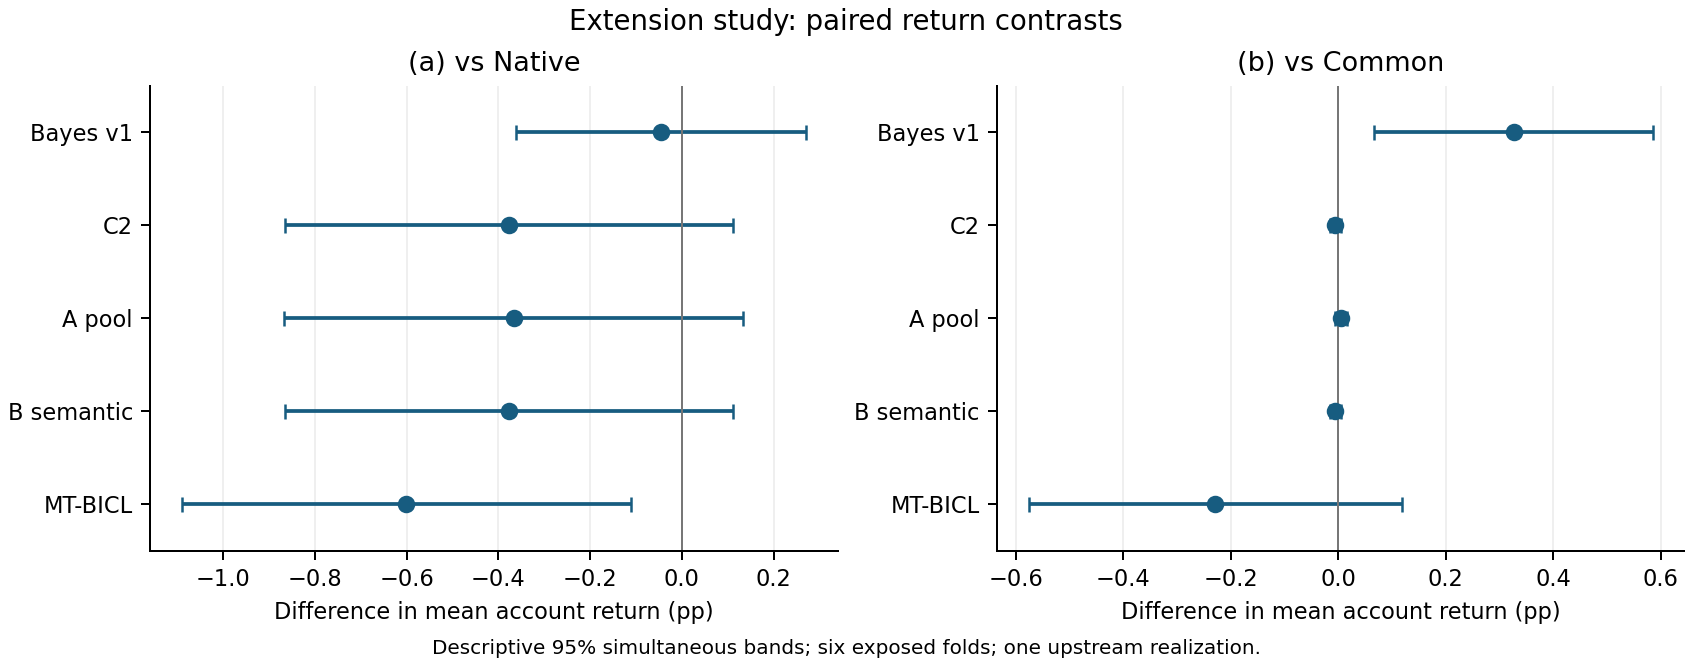
\includegraphics[width=0.78\textwidth,trim=0bp 14.4bp 336.8bp 18bp,clip]{generated/u09/return_contrasts.png}\par\smallskip
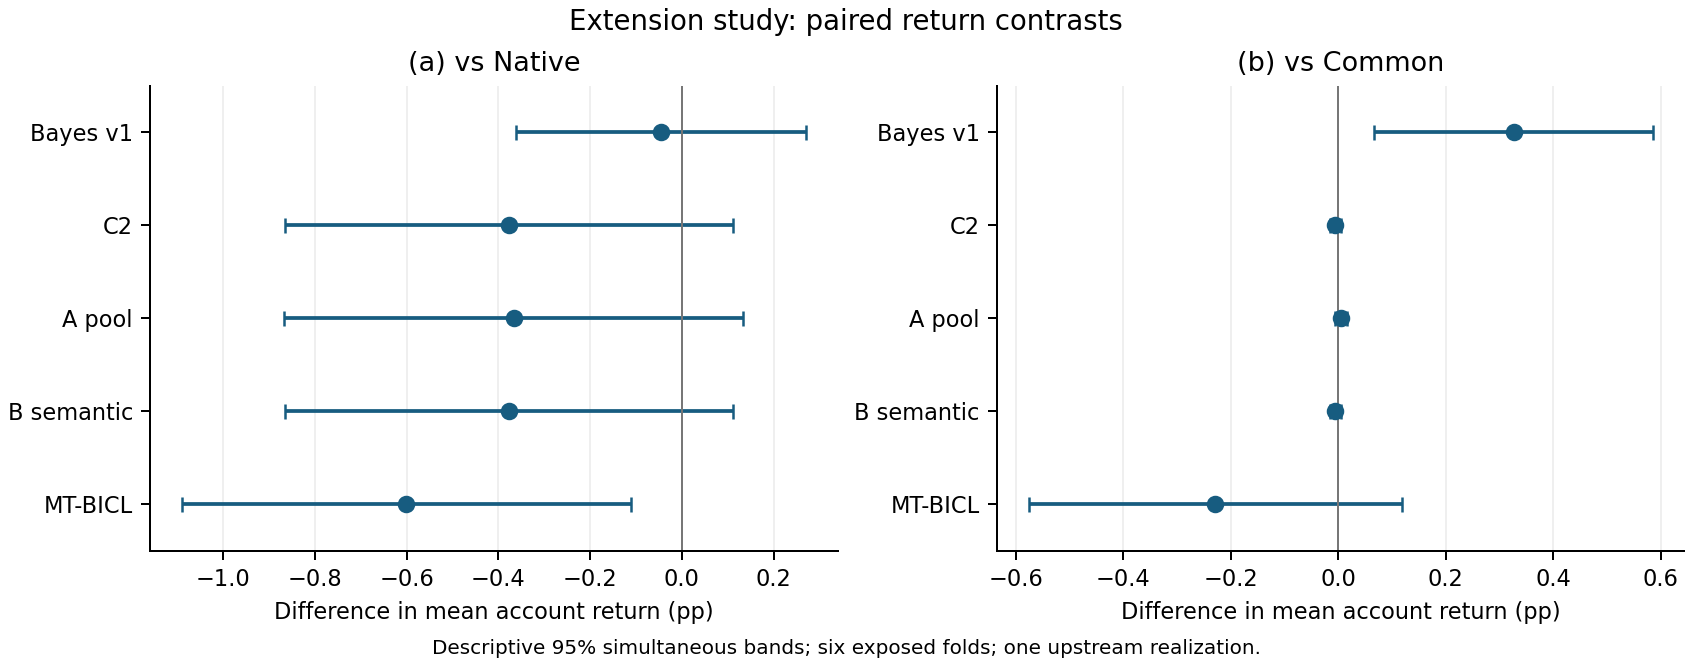
\includegraphics[width=0.78\textwidth,trim=340bp 14.4bp 0bp 18bp,clip]{generated/u09/return_contrasts.png}
\caption{Extension mean account-return contrasts against Native (top) and Common (bottom), in percentage points. The frozen two-panel image is displayed as enlarged panels with separate horizontal scales. Points and descriptive 95\% simultaneous bands come from the paired circular-fold bootstrap (10,000 draws, primary block length L2; joint family of twenty return/BA contrasts). The vertical line denotes zero difference. Bands describe sensitivity on six exposed folds, not calibrated significance or deployable profitability. Both panels retain every extension, including adverse results; uncertainty is conditional on one upstream realization.}
\label{fig:u09-return-contrasts}
\end{figure}

Coverage is part of these method outcomes. C2 and B\_semantic each have only \UnifiedCTwoRaw\ raw Decisions and \UnifiedCTwoBypass\ bypasses per 306 slots; A\_tp\_pool has \UnifiedAPoolRaw\ raw Decisions, Bayesian v1 \UnifiedVOneRaw\ and MT-BICL \UnifiedMTRaw. A fallback reuses the same repeat's parent action and is included in primary metrics, not removed as a failed observation. Table~\ref{tab:u09-support} separates CORE4/OOD5 and recorded effective K; \UnifiedMissingSentiment/\UnifiedPoints\ points have unavailable sentiment. Consequently, near-equal outcomes of C2/B and Common primarily reflect coverage and policy, not evidence that the corresponding retrievers extracted equivalent useful information.

\subsection{Disentangled Alpha--Sentiment Ablation}
\subsubsection{Repeated executions and factorial contrasts}
Table~\ref{tab:repeats} retains all three executions, sample SD, range and cutoff-level prediction disagreement summaries. The two panels have nine market units each but different symbols, dates and prompt families. Their means and SDs are not transferable to the broad 102-unit main study. Zero metric SD does not imply identical predictions: factorial S has unchanged aggregate BA but nonzero disagreement. Return means use nine upstream or eight factorial symbol--block accounts per variant/execution.

On the factorial panel the AS--B BA mean is $-9.52$ pp and AS--P is $-11.90$ pp. Interaction $AS-A-S+B$ is $+14.29$ pp, whereas the gap of mean BA between AS and the observed best single component is zero. These are different quantities. All seven descriptive BA family envelopes contain zero; only 6,986 of 10,000 BA draws retain both classes and 3,014 are undefined. Conditional intervals are not zero-imputed or advertised as calibrated familywise coverage. All factorial mean account returns are negative.

The upstream AS--B mean BA difference is $+4.76$ pp, with conditional percentile interval $[0,10]$ pp. This higher-performing small panel does not replace the main or factorial outcomes. Actual shared reports and paired prompt contents match their frozen parents, but 40 of 147 groups have a successful-call order different from the listed job order, and nine span execution epochs. Routing/quota/resume did not implement full counterbalancing. We retain every outcome and disclose the resulting time/order confounding rather than selecting a clean-looking subset or repairing it retrospectively.
\begin{table}[htb]
\centering\small
\setlength{\tabcolsep}{3pt}
\renewcommand{\arraystretch}{1.15}
\caption{Prediction variability and paired contrasts across three executions of two nine-observation panels.}
\label{tab:repeats}
\textbf{A. Three executions: mean (sample SD)}\par\smallskip
\begin{tabular}{lrrrrr}
\hline
Panel/variant & Acc. (\%) & BA (\%) & BA range & Disagr. (\%) & Return (\%) \\
\hline
U B & 85.19 (16.97) & 90.48 (10.91) & [78.57, 100.00] & 22.22 & 0.37 (0.38) \\
U AS & 92.59 (6.42) & 95.24 (4.12) & [92.86, 100.00] & 7.41 & 0.50 (0.22) \\
F B & 44.44 (11.11) & 28.57 (7.14) & [21.43, 35.71] & 14.81 & -1.70 (0.55) \\
F A & 29.63 (6.42) & 19.05 (4.12) & [14.29, 21.43] & 22.22 & -2.03 (0.31) \\
F S & 22.22 (0.00) & 14.29 (0.00) & [14.29, 14.29] & 22.22 & -2.34 (0.22) \\
F AS & 29.63 (16.97) & 19.05 (10.91) & [7.14, 28.57] & 22.22 & -2.23 (0.63) \\
F P & 48.15 (6.42) & 30.95 (4.12) & [28.57, 35.71] & 14.81 & -1.42 (0.33) \\
\hline
\end{tabular}\par\medskip
\textbf{B. BA contrasts in percentage points}\par\smallskip
\begin{tabular}{lrrrrr}
\hline
Contrast & Mean & SD & Range & Percentile & Family env. \\
\hline
U AS-B & 4.76 & 8.25 & [0.00, 14.29] & [0.00, 10.00] & NA \\
F AS-B & -9.52 & 10.91 & [-21.43, 0.00] & [-22.22, 9.52] & [-37.14, 18.10] \\
F A-B & -9.52 & 4.12 & [-14.29, -7.14] & [-20.37, 14.29] & [-37.14, 18.10] \\
F AS-S & 4.76 & 10.91 & [-7.14, 14.29] & [-6.67, 24.07] & [-22.86, 32.38] \\
F S-B & -14.29 & 7.14 & [-21.43, -7.14] & [-29.63, 10.00] & [-41.90, 13.33] \\
F AS-A & 0.00 & 12.37 & [-14.29, 7.14] & [-20.00, 11.11] & [-27.62, 27.62] \\
F AS-P & -11.90 & 14.87 & [-28.57, 0.00] & [-28.57, 4.76] & [-39.52, 15.71] \\
F interaction & 14.29 & 14.29 & [0.00, 28.57] & [-16.67, 38.89] & [-13.33, 41.90] \\
\hline
\end{tabular}\par\medskip
\begin{minipage}{\textwidth}\footnotesize U/F denote upstream/factorial panels; BA intervals condition on 6,986 finite draws, with 3,014 undefined draws among 10,000 resamples.\end{minipage}
\end{table}


\subsubsection{Extension bridges do not replace missing ablations}
Table~\ref{tab:u09-bridge} distinguishes the native-to-common alpha/prompt bridge, the fact-anchor bridge and the MT revision step. MT agrees with Fact\_Anchor on 302/306 final actions. This limits attribution of the total MT-versus-baseline outcome to the numerical student or retrieved context. The earlier alpha/sentiment/placebo panels remain separate evidence; U09 did not execute retrieval-only, statistics-only, no-prior, no-target or no-utility interventions. Registry support for an ablation is not an observed result. A controlled component study would require its own protocol and executions.

\subsection{Robustness and Sensitivity}
\subsubsection{Temporal and dependence diagnostics}
Table~\ref{tab:temporal} keeps the all-102 primary cohort and two overlapping structural cohorts. The primary Full--Base BA interval is $[\PrimaryLow,\PrimaryHigh]$ pp. The common-eight cohort has 96 units over twelve dates; recent-nine has 54 over six dates. They are sensitivity views, not independent replications or grounds for choosing a more favourable headline. The six-block sample includes an all-DOWN early-2025 block: within-block BA without both classes is undefined rather than fabricated.

Past Close/SMA60 contexts distinguish bull, bear and sideways observations. These are per-security descriptions, not validated market-wide index regimes or a regime-conditioned trading policy. Additional volatility and turnover-proxy thresholds are fitted on purged training data, but their post-inference stratification remains descriptive. Close times Volume is in vendor units, not measured spread/depth liquidity. Exposure based on three target sessions differs from whole-calendar exposure with gaps.

Calendar-aligned HAC accuracy effects for common-eight/recent-nine are $+3.125/+9.259$ pp. At lags 0/1/2, common-eight SEs are 0.026042/0.023146/0.020172 with $p$-values 0.255346, 0.204107 and 0.149610; recent-nine SEs are 0.040713/0.047112/0.045710 with $p$-values 0.072051, 0.106554 and 0.098654. These are accuracy, not BA, effects on twelve/six selected dates. Companion S4 retains all six rows, the calendar masks, all regime strata, block-length sensitivities and leave-one-block-out diagnostics. Few clusters and irregular dates prevent reliable significance, null-effect or calibrated-coverage conclusions.
\begin{table}[!htb]
\centering\small
\setlength{\tabcolsep}{3pt}
\renewcommand{\arraystretch}{1.15}
\caption{Overlapping temporal cohorts and observed trend strata. Small-block intervals and calendar-aligned HAC diagnostics are descriptive rather than calibrated significance tests.}
\label{tab:temporal}
\textbf{A. Cohorts: BA percent; difference/interval in pp}\par\smallskip
\begin{tabular}{lrrrrrrr}
\hline
Cohort & $N$ & Dates & Blocks & Full & Base & $\Delta$ & Interval \\
\hline
All & 102 & 12 & 6 & 52.96 & 49.71 & 3.25 & [-1.18, 8.13] \\
Common eight & 96 & 12 & 6 & 50.69 & 48.61 & 2.08 & [-1.20, 5.26] \\
Recent nine & 54 & 6 & 3 & 53.08 & 46.67 & 6.41 & [0.00, 12.50] \\
\hline
\end{tabular}\par\medskip
\textbf{B. Observed per-security trend contexts (percent)}\par\smallskip
\begin{tabular}{lrrrrrr}
\hline
Trend & $N$ & UP/DOWN & Full BA & Base BA & Full LONG & Base LONG \\
\hline
Bear & 35 & 5/30 & 43.33 & 41.67 & 11.43 & 14.29 \\
Bull & 33 & 9/24 & 47.92 & 53.47 & 36.36 & 39.39 \\
Sideways & 34 & 11/23 & 59.49 & 46.25 & 23.53 & 32.35 \\
\hline
\end{tabular}\par\medskip
\begin{minipage}{\textwidth}\footnotesize Cohorts overlap and are not pooled as extra samples. Trend uses past Close/SMA60 with strict +/-2\% thresholds; it is not an index-regime policy. Primary intervals retain both dates, full cross-sections and pairing within blocks. HAC concerns accuracy rather than BA and is reported for both fixed-universe panels at lags 0/1/2 in S4.\end{minipage}
\end{table}


\subsubsection{Auxiliary numeric selector controls}
Table~\ref{tab:numeric} is a separate numeric study, not an LLM factor-selector ablation. Causal adapters and train-only eligibility, imputation, scaling, orientation and ranking are fitted once per symbol--block scope, then retained through validation/test. Fixed custom five, dynamic train top-five, the same IDs without sign flip, and all twenty random eligible-five trials produce 2,346 predictions on the same 102 units. No random seed is selected after observing results.

Dynamic-minus-fixed, dynamic-minus-random-family and dynamic-minus-no-flip BA differences are respectively $+15.84$, $+7.33$ and $+6.44$ pp. Exact six-block two-sided sign-flip values are 0.0625, 0.125 and 0.53125; Holm correction \cite{holm1979multiple} over all 23 declared hypotheses gives adjusted $p=1$ throughout. Unadjusted percentile intervals and the entire random dispersion remain visible. Positive point differences do not establish superiority, and the no-flip contrast does not identify sign-flip value inside the LLM pipeline.

Native diagnostics separately account for 102 cutoffs, 8,670 candidate opportunities and 510 selected slots. WQ42 occurs at 52/102 cutoffs (52/510 slots); adjacent nonzero IC signs flip 1,282 times over 7,894 eligible transition pairs. These are dependent in-sample diagnostics, not out-of-sample alpha stability. Complete per-factor frequency, eligible denominators, IC signs, windows and all 21 exclusions are retained in the registry companion. Numeric controls do not repair native row-wise noncausality, provide the missing fixed/random LLM experiment, or certify original-expression equivalence.
\begin{table}[!htb]
\centering\small
\setlength{\tabcolsep}{3pt}
\renewcommand{\arraystretch}{1.15}
\caption{Train-fit numeric selector controls using separate causal adapters. These auxiliary results neither repeat the native LLM selector experiment nor repair its row-wise causal defect.}
\label{tab:numeric}
\textbf{A. Pooled numeric results; random mean (SD)}\par\smallskip
\begin{tabular}{lrrrrr}
\hline
Strategy & Trials & Acc. (\%) & BA (\%) & MCC & Random BA range \\
\hline
Fixed custom five & 1 & 49.02 & 39.22 & -0.193 & -- \\
Dynamic train top-five & 1 & 62.75 & 55.06 & 0.093 & -- \\
Same IDs, no flip & 1 & 50.98 & 48.62 & -0.024 & -- \\
Random eligible five & 20 & 51.27 (5.32) & 47.74 (5.38) & -0.039 (0.094) & [37.97, 57.17] \\
\hline
\end{tabular}\par\medskip
\textbf{B. Three primary contrasts; multiplicity family = 23}\par\smallskip
\begin{tabular}{lrrrr}
\hline
Contrast & $\Delta$BA (pp) & Percentile interval & Exact $p$ & Holm $p$ \\
\hline
Dynamic - fixed & 15.84 & [6.82, 25.22] & 0.0625 & 1.0000 \\
Dynamic - random mean & 7.33 & [0.57, 13.75] & 0.1250 & 1.0000 \\
Dynamic - no flip & 6.44 & [-10.93, 20.26] & 0.5312 & 1.0000 \\
\hline
\end{tabular}\par\medskip
\begin{minipage}{\textwidth}\footnotesize $N=102$, UP/DOWN=25/77, 51 train-fit scopes. Numeric adapters/preprocessing are separate from the native LLM pipeline. All 20 random trials and all 23 contrasts remain in S3. Exact tests have 64 six-block sign assignments; percentile intervals are unadjusted, Holm uses the full 23-hypothesis family. No contrast rejects at 0.05.\end{minipage}
\end{table}


\subsubsection{Extension repeat, support and resampling sensitivity}
Table~\ref{tab:u09-repeats} retains all three Decision repeats on the full extension support. The uncertainty is conditional on one shared upstream realization; it does not estimate upstream-by-Decision variance or increase the number of market dates. \ref{app:additional} reports both L1/L3 variants beside primary L2, and the predeclared CORE4 subset. Leave-one-fold/symbol-out effects and every per-symbol/fold/repeat classification/account row remain in the machine-readable companions. These views retain the observed eligibility mask, including BHN's three recent folds, rather than padding missing accounts with CASH. No favorable block length, subgroup, repeat or student checkpoint is selected after examining U09 outcomes. Bands remain descriptive on the exposed cohort.

\section{Limitations and Future Work}
\label{sec:limitations}

\subsection{Limitations}
\paragraph{Component attribution}
Full--Base changes factor and sentiment content together with prompt length. Compact reports in the main/upstream panel also differ from the explicit factor rows in the factorial panel. The placebo uses one predetermined past donor, and only nine market units support each repeated component panel. These differences limit attribution of forecast changes to specific information sources. The historical-context study includes no retrieval-only, statistics-only, no-prior, no-target or no-utility intervention.

\paragraph{Factor construction and sentiment validity}
Native backward filling, whole-Series normalization and volume-availability branching can make an earlier historical row depend on later rows within the supplied prefix. Isolation from prices after the current decision cutoff therefore coexists with noncausal historical diagnostics. Native orientation and ranking also reuse their calibration observations. The causal projection and numerical controls use separate constructions, so their results apply to those constructions. Six selected metadata slots differ from their handler descriptions, and the semantic effect of these mismatches is unmeasured.

Historical news content and publication availability are not independently authenticated, and no financial-domain sentiment test set or annotation agreement is available. Unknown legacy scores and locally rescored excerpts have different provenance. Missing sentiment, including 79/102 historical-context points, reduces the information actually available to the methods. Bank and query return calculations also differ numerically in 828/852 bank records, with maximum absolute discrepancy about 0.042988489 percentage points; this comparison concerns returns rather than a count of label changes.

\paragraph{Sampling and model variability}
The nine equities form a purposive sample with unverified point-in-time listing, delisting and suspension membership. Twelve selected dates and six correlated temporal blocks provide limited independent market evidence. Model-training contamination is possible because outcomes precede the data freeze. The schedule was finalized after some inference, and hosted routing, call order and serving revisions introduce further uncertainty. Three Decision repeats conditional on one upstream realization do not measure full-system variability or add market dates.

\paragraph{Historical support and action policy}
The 852-example prior bank covers four stocks. Conditional and explicit-count priors each generate only three new Decisions per 306 slots, while the trend--pattern prior generates 24. MT-BICL agrees with its fact anchor on 302/306 final actions. Consequently, aggregate results include substantial fallback and anchor retention. Native--Common changes both alpha projection and instructions, and the fact anchor adds another intervention; overall differences cannot be assigned to retrieval or student inference alone.

\paragraph{Execution and visual interpretation}
Negative account means provide no evidence of a deployable profitable strategy. Fractional fills, fixed fees/slippage, settlement phases, lot/capacity limits and volume units are assumptions or proxies. Corporate actions, price-limit queues, spreads, depth and partial fills are unverified, and separate accounts omit portfolio capital competition. Chart geometry and consistency checks constrain inputs and obvious contradictions, while local visual grounding remains untested. Prompt priorities likewise provide heuristic rather than learned evidence weighting.

\subsection{Future Work}
A prospective study should correct native row causality, repeat selection and preprocessing within chronological training, and reserve an untouched evaluation interval. Candidate search can be assessed with White's Reality Check or Deflated Sharpe analysis \cite{white2000reality,bailey2014deflated}. Broader stock/date coverage, authenticated historical inputs and independently regenerated upstream realizations would improve inference. Prior/retrieval/MT ablations, financial-news annotations and matched counterfactual charts would test component mechanisms, while portfolio simulation requires venue-specific execution data.

\subsection{Broader Impact}
Financial decision support can make heterogeneous evidence accessible, but fluent reports may overstate the reliability of sparse or contradictory inputs. Forecast confidence should therefore remain distinct from action policy and realised account performance. Use and distribution of news, price data and model assets must also respect their respective licences and source terms.

\section{Conclusion}
\label{sec:conclusion}

This paper integrates OHLCV alpha factors, Vietnamese sentiment and historical context into a multi-agent decision-support system. Shared upstream reports support paired comparisons, while explicit eligibility, fallback and utility rules connect model proposals to long-only account actions.

On 102 component-study observations, Full BA is \FullBA\%, Base \BaseBA\% and the price-only logistic comparator \LogisticPriceBA\%. Full and Base identify the same seven UP outcomes, with Full reducing false LONG forecasts; mean account returns are \FullReturn\% and \BaseReturn\%. In the historical-context study, Bayesian-prior return differs from Common by $+\UnifiedVOneCommonReturnEffect$ percentage points and from Native by $\UnifiedVOneNativeReturnEffect$ points. Native, Common, Bayesian prior and MT-BICL return \UnifiedNativeReturn\%, \UnifiedCommonReturn\%, \UnifiedVOneReturn\% and \UnifiedMTReturn\%, respectively.

Information integration changes recorded decisions, but the evidence does not establish stable predictive superiority, causal component value or deployable profitability. Limited dates, native within-history noncausality, uncertain news validity and support-dependent action reuse constrain interpretation. Prospective experiments with causal inputs, broader temporal coverage, repeated upstream realizations and targeted component interventions are needed to assess generalisation.


%% CRediT authorship contribution statement
%% (elsarticle.cls has no \credit/\printcredits macros; the CRediT
%% roles from the original cas-sc source are preserved here verbatim
%% as a standard Elsevier "CRediT authorship contribution statement"
%% section instead.)
% \section*{CRediT authorship contribution statement}

% \textbf{Van-Tang Nguyen:} Conceptualization (C); Software (So); Validation (Va); Investigation (I); Original draft preparation (O); Project administration (P); Funding acquisition (Fu).

% \textbf{Hoang-Dung Phan:} Methodology (M); Software (So); Formal analysis (Fo); Investigation (I); Resources (R); Data curation (D); Original draft preparation (O); Writing-review and editing (E); Visualization (Vi); Supervision (Su).

% \textbf{Thanh-Tam Do Thi:} Methodology (M); Investigation (I); Data curation (D); Original draft preparation (O); Writing-review and editing (E); Supervision (Su).

% \textbf{Phuong-Thai Nguyen:} Methodology (M); Investigation (I); Data curation (D); Original draft preparation (O); Visualization (Vi); Supervision (Su).

% \textbf{Hong-Viet Tran:} Conceptualization (C); Methodology (M); Software (So); Validation (Va); Formal analysis (Fo); Data curation (D); Original draft preparation (O); Writing-review and editing (E); Project administration (P).

\section*{Declaration of competing interest}
Authors state no conflict of interest.

% \section*{INFORMED CONSENT (if applicable)}
% The protection of privacy is a legal right that must not be breached without individual informed consent. In cases where the identification of personal information is necessary for scientific reasons, authors should obtain full documentation of informed consent, including written permission from the patient prior to inclusion in the study. Incorporate the following (or a similar) statement: We have obtained informed consent from all individuals included in this study.

% \section*{ETHICAL APPROVAL (if applicable)}
% When papers talk about using people or animals, authors should make it clear that the research followed all national rules and institutional policies, and it was approved by the authors' institutional review board or a similar committee. The Helsinki Declaration's tenets must guide all investigations involving human subjects. Authors must also identify the committee or review board approving the experiments and provide a statement indicating approval of the research. Incorporate the following (or a similar) statement: The research related to human use has been complied with all the relevant national regulations and institutional policies in accordance with the tenets of the Helsinki Declaration and has been approved by the authors' institutional review board or equivalent committee; or: The research related to animal use has been complied with all the relevant national regulations and institutional policies for the care and use of animals.

\section*{Data and code availability}
The \href{https://github.com/DungPhanHoangg05/A-Multi-Agent-Large-Language-Model-Approach-to-Price-Driven-Stock-Trading-in-the-Vietnamese-Stock-Ma}{project repository} records the implementation and earlier result artifacts. The final reproducibility package and scientific companions S1--S4 have been prepared as a private local draft. Public distribution rights and a persistent archive identifier remain pending; no DOI or public availability of the full package is asserted. OHLCV/news snapshots are reconstructed research inputs rather than authenticated submission-time data. Distribution remains subject to source terms, news copyright, model licences and permissions; the upstream QuantAgent MIT notice does not grant rights over all additions or data.

Companion S1 contains \texttt{S1\_classification.csv}, \texttt{S1\_per\_class.csv} and \texttt{S1\_macro.csv}; S2 contains all executions, contrasts and disagreements; S3 contains numeric metrics, random trials and the full family; S4 contains calendar, HAC, block sensitivity, regimes and dependence diagnostics. Exact source paths and hashes are recorded in the manuscript release. The private raw package separately retains inputs, messages/images, responses/errors, parse/checkpoints, pins and provenance.

\begingroup\emergencystretch=2em
The separately identified U08/U09 study and its presentation release have separate bindings for inputs, receipts and manifests (\ref{app:software}). U09's verified \texttt{results.json}, summary, contrasts, bridges, support and sensitivity companions underlie the extension tables. Their presentation manifest is \path{outputs/revision/u09_manuscript_assets_v1/manifest.json}. The earlier manuscript handoff, sources and request-level reviewer crosswalk are bound by \path{outputs/revision/manuscript_unified_final_v1/manifest.json}. The present layout and reference revision has separate sources and page locators under \path{outputs/revision/manuscript_layout_references_v1/manifest.json}. Exact-byte historical restoration and offline metric replay are documented in the repository without promising identical newly hosted responses. These local releases confer no public identifier, redistribution rights or editorial acceptance.
\par\endgroup


\section*{Acknowledgments}
This research is funded by Foreign Trade University under research program number FTURP02-2026-08


%% ── APPENDIX ──────────────────────────────────────────────────────────────────


\FloatBarrier
\appendix
\section{Agent System Prompts}
\label{app:prompts}
This appendix specifies the role-level prompt and output contracts used to interpret the system. The summaries below are English explanations of the actual Vietnamese prompt families, not new verbatim templates or translations claimed to be identical to each archived request. Exact messages, image payloads and request metadata remain in the companion archive. The evaluated path must be distinguished from optional prompts present in general live-mode code.

\subsection{Decision Agent Prompt}
\label{app:prompt_decision}
The prompt supplies distilled Indicator, Pattern and Trend reports with variant-enabled factor and sentiment sections. It requests comparison of trend/key levels, candles, momentum and enabled quantitative/text evidence, followed by a forced LONG/SHORT forecast for the net next-open/target-close cycle. The output contract comprises direction, horizon, confidence, risk/reward, supporting/opposing evidence and justification. General instructions remain in Base, while both factor and sentiment sections are removed. Main compact factor text and factorial five-row text are different families. Section~\ref{sec:systemarchitecture} and Figure~\ref{fig:decision_agent} describe these distinctions; the exact archived request is authoritative.

\paragraph{Extension common/prior projection}
Common uses the same shared Indicator/Pattern/Trend and sentiment parent as Native but substitutes the frozen causal alpha report and a common instruction/schema. Prior branches prepend only the visible historical evidence allowed by their readiness trace. Bayesian v1 displays at most three matured same-symbol examples. C2 conditions its rate estimates on matched Trend/Pattern/Alpha/Indicator signals; A conditions the statistics on Trend/Pattern; B renders C2's counts, plug-in credible intervals and example IDs with explicit semantic definitions. The English descriptions here summarize those request builders, not verbatim served prompts. Every actual Vietnamese prompt, prefix/source hash and structured-output schema remains authoritative in the U08 raw/preparation records.

For C2/A/B, the frozen readiness policy requires population support at least 20; a displayed statistic additionally requires conditional support at least five and credible-interval width at most 0.75. Example readiness is tested separately, with feature/scaler availability and qualified selected IDs. Selection uses requested K=3, seed 42, signal weight 0.5, 365-day recency half-life, maximum age 730 days, similarity threshold 0.625 and minimum five-session spacing. A prompt can show a qualified statistics or examples block without claiming that the other is ready. An empty visible block reuses Common's completed action. These historical evidence gates do not impose a profitability threshold on the current query.

\paragraph{Fact and MT context}
Fact\_Anchor receives the common reports, deterministic fact identifiers and assertions, and Common's completed reply; its reply must reproduce the fact assertions. The MT request adds a source-bound anchor, prior and target summaries, compact exemplars, query features, student probability and teacher-based utility summary where eligible. A source card binds the common request, fact card and anchor replies. Each context prefix is at most 600 characters, and the final request remains strictly below 6,500 characters after report distillation and capping. A bypass has neither a fabricated request nor a fabricated raw reply. Fact verification checks declared identifiers and enums, not every free-text financial claim; the external policy, rather than prompt wording alone, enforces the utility decision rule.

\subsection{Pattern Agent Prompt}
\label{app:prompt_pattern}
The visual input is the archived candlestick PNG. The requested report covers pattern, confidence, directional bias, evidence, key candles and implication. The body-colour convention is green for Close greater than Open and red otherwise, including doji. This instruction and the deterministic consistency flag do not establish that the model grounded its answer in local chart evidence.

\subsection{Trend Agent Prompt}
\label{app:prompt_trend}
The trend input is a separate PNG with support/resistance annotations. The requested report covers direction, support, resistance, line slope, price relative to support, detailed analysis, forecast and confidence. Support is blue and resistance red in the corrected input. Actual Vietnamese wording, inherited high-frequency language and unknown semantic compliance remain documented; an English summary does not remove those limitations.

\subsection{Indicator Agent Prompt}
\label{app:prompt_indicator}
The software contains an optional LLM reporting path, but the evaluated backtest returns a deterministic report without that LLM call. The five votes, counts and heuristic confidence are generated numerically. Treating the optional prompt as an observed study request would misdescribe both the input contract and call cost. The rules used here are in \ref{app:indicator_logic}.

\subsection{Sentiment LLM Prompt (Subroutine of Alpha Agent)}
\label{app:prompt_sentiment}
The frozen sentiment path uses saved classifier scores and aggregate/count fields. It does not establish that an LLM read a peer/article corpus in this experiment. Scorer identity, the probability-difference score, decay and unavailable peer fields are specified in Section~\ref{sec:formulation}. Optional crawler/LLM capabilities in the application are not substituted for missing frozen inputs.

\subsection{Alpha Agent LLM Reasoning Prompt}
\label{app:prompt_alpha}
An optional live-mode reasoning prompt exists, but the frozen numerical/report path bypasses an additional Alpha reasoning call. The enabled factor rows and skill fields are delivered to Decision using the recorded family. We consequently describe an Alpha role rather than claiming a separate model interpreted every selected factor before Decision.

\FloatBarrier
\section{LangGraph State Schema}
\label{app:state_schema}
The declared \texttt{IndicatorAgentState} is a shared \texttt{TypedDict}; the backtest wrapper and individual nodes determine which fields are actually populated. Inputs include \texttt{kline\_data}, \texttt{time\_frame}, \texttt{stock\_name}, \texttt{is\_backtest}, \texttt{point\_in\_time\_df}, \texttt{as\_of\_date}, language and the two image payloads. Report fields are \texttt{indicator\_report}, \texttt{alpha\_report}, \texttt{pattern\_report}, \texttt{trend\_report} and \texttt{sentiment\_report}; sentiment data/normalizer fields and message history are distinct from those reports. Final output fields include \texttt{decision\_prompt} and \texttt{final\_trade\_decision}.

Declared RSI/MACD/Stochastic/ROC/Williams, ATR, Bollinger and ADX/DI arrays do not imply that every array is forwarded by the deterministic backtest Indicator node or that each is a separate vote. Likewise, a sentiment schema comment does not establish that its peer or relative fields were observed. The forecasting target is the net Open-to-Close cycle in Eq.~\ref{eq:label}; it is separate from the state schema's field names. The evaluated pair shares upstream report parents, then uses variant-specific Decision composition and separate ledgers. The full schema listing and wrapper provenance are retained in source rather than reproduced as a misleading complete runtime trace.

\paragraph{Extension records and outcome barrier}
\texttt{SharedSnapshot} binds point/symbol/cutoff/fold, realization, payload and provenance. Its payload retains the report/image parent and the separately hash-bound causal alpha projection. A forecast record adds variant/profile, repeat, request/source identity, optional raw reply and preparation/retrieval trace. A policy record distinguishes \texttt{raw\_proposal}, \texttt{final\_action}, reason, bypass and anchor/utility proof. \texttt{prepare} and \texttt{forecast} records are durable for all eight roles and three repeats before an outcome record is admitted. The canonical outcome carries explicit decision/entry/exit fields and Eq.~\ref{eq:label} metadata; it is not part of the forecasting state. Duplicate raw UUID reuse, missing dependencies or source/data mismatches are errors, not imputed actions. U09's \texttt{results.json} and artifact bindings summarize the sealed active grid; the older replay API's singular \texttt{result.json} is a different schema.

\FloatBarrier
\setcounter{table}{0}
\section{Custom Alpha Formula Implementation}
\label{app:signals}
The custom formulas below specify native handlers and distinguish their preprocessing from prototype/fallback implementations. ``Custom'' describes their role in this implementation; it is not a validated novelty or profitability claim. The following formulas precede native global normalization and IC orientation. Handler identities are not the rank of a selected display row.
\begin{table}[!htb]
\centering\small
\setlength{\tabcolsep}{3pt}
\renewcommand{\arraystretch}{1.15}
\caption{Custom native factor definitions and implementation distinctions.}
\label{tab:custom_definitions}
\textbf{Before global normalization and IC orientation}\par\smallskip
\begin{tabular}{lp{8.0cm}p{5.0cm}}
\hline
ID & Native handler expression & Distinction \\
\hline
FDM & $\tanh(0.5\,a_t V_t/ADV_{20,t})$ & Native uses adjusted one-bar return, not the MACD display template. \\
SFA & $\tanh(1.5\tanh(H_t/(0.005C_t+\epsilon))+0.5a_t)$ & Native uses MACD histogram and return, not sentiment; prototype has a distinct sentiment branch. \\
LVR & $\tanh(-0.8\,z_{20}((C_t-SMA_{5,t})/C_t))$ & Rolling mean/SD conventions and partial windows are implementation-specific. \\
BFE & $\tanh(1.5(\%B_t-0.5)\,VolZ_{5,t})$ & Negative VolZ reverses the sign; zero cancels. No squeeze or volume-expansion gate. \\
OFE & $\tanh(3a_t\,CP_t)$ & OHLCV proxy, not measured signed order flow. \\
\hline
\end{tabular}\par\medskip
\begin{minipage}{\textwidth}\footnotesize $a_t$ is one-bar pct-change divided by rolling 20-bar sample SD (minimum five); $H_t$ is MACD(12,26,9) histogram; $CP_t$ is close location relative to the bar midpoint/range; ADV is mean Volume, not dollar volume. Guarded denominators and fills follow the registry. BFE registry sample-SD preprocessing differs from the rounded/population-SD prototype. Six selected metadata slots differ from their handler description, without the literal wrong formula in the affected prompts. A display rank of four does not identify BFE. Full expressions, guards and counterexamples are in the companion registry.\end{minipage}
\end{table}


\paragraph{Common operators are a separate profile}
The extension retains the native formulas above and in the archived registry. Its row-causal adapters remove backward fills, use only row-available rolling information and keep warm-up/missingness explicit. Training fixes IC orientation; purged validation selects five factor IDs and a threshold from $\{0.05,0.10,0.20\}$. The frozen policy requires at least 60 train observations, 30 validation observations and five validation LONG cycles. Fixed historical origin, query-prefix hash and selector identity are checked on every projection. This profile does not replace the native full-Series normalization in Eq.~\ref{eq:alpha_norm}, and a handler name does not assert equivalence between the two constructions.

\subsection{Flow-Driven Momentum (FDM)}
FDM multiplies volatility-adjusted one-bar return by a volume/ADV20 ratio before the scaled tanh. The return adjustment uses rolling sample SD with its implementation-specific minimum observations. It is an OHLCV proxy, not directly measured order flow.

\subsection{MACD/Return Proxy (SFA)}
The native SFA handler combines a normalized MACD histogram and adjusted return. Its name/description and the earlier MACD-Flow display template do not substitute for the handler. No sentiment variable enters this native formula; the prototype has a separate sentiment branch.

\subsection{Liquidity Void Reversion (LVR)}
LVR applies a rolling z-score to the Close--SMA5 deviation divided by Close, with a negative multiplier before tanh. Guarded denominators, rolling windows, partial samples and sample-SD conventions are retained from the implementation.

\subsection{Bollinger Squeeze \& Flow (BFE)}
BFE uses $\tanh(1.5(\%B-0.5)VolZ_5)$. Negative volume z-score reverses the sign, and zero cancels it. There is no volume-expansion or squeeze gate in this formula. Registry preprocessing uses sample SD and differs from the rounded/population-SD prototype; they are not treated as interchangeable.

\subsection{Order Flow Exhaustion (OFE)}
OFE combines adjusted return with the close location relative to the bar midpoint/range. The name does not authenticate signed trade flow. Its guarded OHLCV expression and subsequent native normalization remain part of the actual signal definition.

\FloatBarrier
\setcounter{table}{0}
\section{Indicator Signal Classification Logic}
\label{app:indicator_logic}
\begin{table}[!htb]
\centering\small
\setlength{\tabcolsep}{3pt}
\renewcommand{\arraystretch}{1.15}
\caption{Indicator signal rules and missing-data conventions.}
\label{tab:indicator_rules}
\textbf{Five deterministic votes}\par\smallskip
\begin{tabular}{lp{7.1cm}p{5.2cm}}
\hline
Signal & Priority and boundaries & Qualification \\
\hline
MACD & Previous strict/current inclusive crossing first; otherwise histogram sign and change. & 12/26/9; no Stochastic histogram. \\
RSI & $\ge70$: bear; $\le30$: bull; $55\le x<70$: bull; $30<x\le45$: bear. & 45--55 uses change against the third retained sample. \\
Stochastic & Crossing precedes $\ge80$ bear / $\le20$ bull; interior fallback retained. & Legacy equality/zero-D truthiness is disclosed. \\
Williams \%R & $\ge-20$: bear; $\le-80$: bull; otherwise retained-sample direction. & Not a volatility vote. \\
ROC & $>+0.5\%$: bull; $<-0.5\%$: bear; equality neutral. & Thresholds follow four-decimal rounding. \\
\hline
\end{tabular}\par\medskip
\begin{minipage}{\textwidth}\footnotesize None/nonfinite values are removed, zero retained; rounding is to four decimals before classification. Retained samples need not be consecutive if missing. Missing/error gives a neutral vote within denominator five. Directional plurality, ties MIXED, and confidence are heuristics, not calibrated probabilities.\end{minipage}
\end{table}

\subsection{MACD Classification}
Previous strict/current inclusive line crossing is checked before histogram sign/change. Parameters are 12/26/9. A Stochastic oscillator has no MACD histogram; the two rules must not be conflated.
\subsection{RSI Classification}
The ordered extreme branches ($\ge70$ bearish, $\le30$ bullish) precede interior trend bands. Thus $55\le RSI<70$ is bullish and $30<RSI\le45$ bearish; the middle interval uses change against the third retained observation. The ordered branches make the extreme and interior regions mutually exclusive.
\subsection{Stochastic Oscillator Classification}
Crossing has priority over overbought/oversold thresholds. Legacy equality and zero-D truthiness behaviour is retained and disclosed rather than replaced retrospectively with an idealized oscillator rule.
\subsection{Williams \%R Classification}
Values $\ge-20$ are bearish and $\le-80$ bullish before the interior retained-sample direction rule. This is a bounded momentum indicator, not a volatility measure.
\subsection{ROC Classification}
After four-decimal rounding, ROC greater than $+0.5\%$ is bullish, below $-0.5\%$ bearish, and equality is neutral.
\subsection{Consensus Rule}
Nonfinite samples are removed while zero is retained; retained observations need not be consecutive. Missing/error votes are neutral in denominator five. Directional plurality, a mixed tie and heuristic confidence are distinct from a requirement that every directional vote have a strict majority. None is a calibrated forecast probability.

\FloatBarrier
\section{Software Dependencies and Reproducibility}
\label{app:software}
The research runtime is Python 3.13.5 with pinned numerical, graph, model-client and chart dependencies recorded in the reproducibility package. The local sentiment-model backend uses Transformers \cite{wolf2020transformers}. Indicator calculations use TA-Lib; chart images and numerical diagnostics have their own source hashes. Raw actual prompts, callback/error records, retry/checkpoint state, provider aliases and model/scorer assets are retained separately from scientific companion tables. Local saved-prediction replay reproduces metric calculations, not newly served model outputs or historical news availability.

The operational installation, Flask/JSON handling, tokenizer configuration and optional endpoint routing instructions remain in the repository. Their existence does not establish that each backend was used in the frozen study. Public distribution remains conditional on rights and a real persistent identifier. No credentials or private review document belong in a public reproducibility package.

\paragraph{Extension tasks, teacher and frozen student}
The numerical context uses same-symbol 63-session tasks, up to three prior tasks and at most eight matured observations per task and target, with prior/target/query IDs and holding intervals disjoint. Four numerical coordinates encode momentum over five/twenty sessions, twenty-session volatility and relative position to the twenty-session moving average; their train-fitted scaler and clipped model representation are frozen. Factual buckets use the signs of MACD minus signal and Close minus SMA20; exact zero/missing axes produce UNKNOWN rather than a favorable bucket. Query outcomes are absent. Context is frozen before each fold's first query and excludes all 102 test IDs across folds.

The explicit teacher uses conjugate Bayesian updating \cite{gelman2013bayesian} with sixteen Beta components on $\mu\in\{0.2,0.4,0.6,0.8\}$ and $\kappa\in\{2,8,32,128\}$, with $\alpha=\mu\kappa$, $\beta=(1-\mu)\kappa$ and train-only MAP-EM mixture weights, using expectation--maximization \cite{dempster1977em}. Prior-task likelihoods preserve task boundaries; target successes/failures update the target posterior. The selected causal-mask student uses task/role markers and only observed context labels; its query label is masked. The served checkpoint is fixed at seed 42/step 3000. No checkpoint is selected from U09 returns. Utility support requires at least two prior tasks and at least five observed gains and five losses across the admitted magnitude support. Its 4,096 draws use teacher-posterior success probabilities and Bayesian-bootstrap net gain/loss magnitudes \cite{rubin1981bootstrap}. Student $P(y=+1)$ is supplied as context, not substituted for teacher utility draws. Neither procedure is fitted again during U08 inference or manuscript generation.

\begingroup\emergencystretch=2em
\paragraph{Release identities and historical restore}
The protocol and resource manifest are \path{unified_comparison_protocol_v2.json} and \path{unified_comparison_manifest_v2.json} under \path{docs/plan/week12/}. The same directory holds U08's sealed \path{unified_live_research.zip}, U09's \path{unified_analysis_results.zip} and \path{unified_analysis_acceptance.json}. The study locks Python 3.13.5 and 107 package versions, 51 selector bindings, HMM, scaler, teacher and student, with separate bank and query provenance. Regime snapshots use VN-Index observations available by the cutoff, prefix-only forward filtering and recorded fit and training-end dates; future smoothing is excluded. These are historical pins for inputs, weights and source; they are not immutable hosted-weight attestations.

The presentation release \path{outputs/revision/u09_manuscript_assets_v1/manifest.json} binds tables, an English-labelled figure and \texttt{Unified} macros; \texttt{numeric\_cells.json} records literal values, units, scale and rounding. Original Full/Base macros and archives remain intact. The snapshot and \path{docs/plan/week12/final_evidence_map.md} specify historical checkout, exact-byte overlay, restore of 286 ignored assets and cold replay of fifteen U09 artifacts. Verification covers saved predictions and its declared source/runtime release, not identical hosted responses or changed serving code.
\par\endgroup

\FloatBarrier
\setcounter{table}{0}
\section{Additional Account and Symbol Results}
\label{app:additional}
These tables use the same final supports and unchanged predictions as the main results. Supplement S1 gives every baseline by symbol and both classes; S2 contains all execution rows/contrasts; S3 the complete numeric/random family; S4 all temporal/regime/HAC diagnostics. They are scientific companion tables, distinct from raw execution logs and implementation files. No additional market observation is created by these alternative tabulations.
% Cho phép bảng nổi trong phụ lục hiện hành để tránh khoảng trắng do cố định vị trí.
\begin{table}[htb]
\centering\small
\setlength{\tabcolsep}{3pt}
\renewcommand{\arraystretch}{1.15}
\caption{Full and Base classification performance by stock.}
\label{tab:symbol_results}
\textbf{Percent except MCC}\par\smallskip
\begin{tabular}{lrrrrrr}
\hline
Symbol/variant & UP/DOWN & Acc. & BA & MCC & $R_U$ & $R_D$ \\
\hline
BHN/Full & 1/5 & 100.00 & 100.00 & 1.000 & 100.00 & 100.00 \\
BHN/Base & 1/5 & 66.67 & 80.00 & 0.447 & 100.00 & 60.00 \\
CMG/Full & 3/9 & 66.67 & 44.44 & -0.174 & 0.00 & 88.89 \\
CMG/Base & 3/9 & 75.00 & 61.11 & 0.258 & 33.33 & 88.89 \\
FPT/Full & 2/10 & 66.67 & 40.00 & -0.200 & 0.00 & 80.00 \\
FPT/Base & 2/10 & 50.00 & 30.00 & -0.316 & 0.00 & 60.00 \\
HVN/Full & 2/10 & 66.67 & 60.00 & 0.158 & 50.00 & 70.00 \\
HVN/Base & 2/10 & 66.67 & 60.00 & 0.158 & 50.00 & 70.00 \\
MBB/Full & 5/7 & 50.00 & 48.57 & -0.029 & 40.00 & 57.14 \\
MBB/Base & 5/7 & 58.33 & 55.71 & 0.120 & 40.00 & 71.43 \\
MWG/Full & 4/8 & 58.33 & 56.25 & 0.120 & 50.00 & 62.50 \\
MWG/Base & 4/8 & 50.00 & 50.00 & 0.000 & 50.00 & 50.00 \\
VCB/Full & 4/8 & 58.33 & 50.00 & 0.000 & 25.00 & 75.00 \\
VCB/Base & 4/8 & 50.00 & 37.50 & -0.316 & 0.00 & 75.00 \\
VJC/Full & 4/8 & 58.33 & 43.75 & -0.213 & 0.00 & 87.50 \\
VJC/Base & 4/8 & 50.00 & 37.50 & -0.316 & 0.00 & 75.00 \\
VNM/Full & 0/12 & 83.33 & NA & NA & NA & 83.33 \\
VNM/Base & 0/12 & 83.33 & NA & NA & NA & 83.33 \\
\hline
\end{tabular}\par\medskip
\begin{minipage}{\textwidth}\footnotesize BHN contributes six observations and other stocks twelve; NA indicates missing-class support or a degenerate metric.\end{minipage}
\end{table}

\begin{table}[!htb]
\centering\small
\setlength{\tabcolsep}{3pt}
\renewcommand{\arraystretch}{1.15}
\caption{All twelve account-execution sensitivities on unchanged predictions.}
\label{tab:execution}
\textbf{Means over 51 accounts per variant}\par\smallskip
\begin{tabular}{lrrrrr}
\hline
Scenario & Base (\%) & Full (\%) & $\Delta$Full (pp) & Stock & Pending \\
\hline
reference & -0.750 & -0.797 & 0.000 & 0 & 0 \\
pending\_t2 & -0.750 & -0.797 & 0.000 & 0 & 0 \\
advance\_on\_demand & -0.750 & -0.797 & 0.000 & 0 & 0 \\
advance\_auto & -0.803 & -0.840 & -0.043 & 0 & 0 \\
lower\_cost & -0.526 & -0.612 & 0.185 & 0 & 0 \\
higher\_cost & -1.249 & -1.211 & -0.414 & 0 & 0 \\
sell\_charge\_10bp & -0.805 & -0.843 & -0.046 & 0 & 0 \\
no\_fill\_proxy & -0.659 & -0.803 & -0.006 & 0 & 0 \\
delayed\_proxy & -0.621 & -0.766 & 0.030 & 0 & 0 \\
lot100\_cap1pct & -0.602 & -0.745 & 0.052 & 0 & 0 \\
combined & -1.074 & -1.166 & -0.369 & 0 & 0 \\
all\_entries\_missed & 0.000 & 0.000 & 0.797 & 0 & 0 \\
\hline
\end{tabular}\par\medskip
\begin{minipage}{\textwidth}\footnotesize Stock/Pending count Full accounts with residual shares/receivables; zero Full residuals do not imply none for other strategies. All 6,120 account executions are in the companion results. Fee/slippage, advance fees, sell charge, lots and capacity are assumptions. No-fill/delay proxies do not measure queue fills; all entries missed is not a mathematical worst bound.\end{minipage}
\end{table}

\FloatBarrier

\paragraph{Separate extension companions}
The following tables belong only to the U08/U09 extension study. They do not extend the original study's response sample or apply its twelve execution stress scenarios to untested methods. U09 companions preserve 1,530 account rows (ten roles/controls, 51 accounts and three repeats), per-symbol/fold/repeat classification, raw-versus-final actions, policy reasons and prior traces. NA/null values, missing-class reasons and unrecorded effective K remain explicit. The source archive also retains cycle and daily-NAV ledgers; separate account means are not aggregate portfolio returns.
\begin{table}[!htb]
\centering\small
\setlength{\tabcolsep}{3pt}
\renewcommand{\arraystretch}{1.12}
\caption{Extension study: class-aware metrics on the same 102 market points.}
\label{tab:u09-classification}
\textbf{Mean of per-repeat metrics}\par\smallskip
\begin{tabular}{lrrrrrr}
\hline
Role & Acc. (\%) & BA (\%) & MCC & $F1_U$ (\%) & $F1_D$ (\%) & Macro F1 (\%) \\
\hline
Native & 65.36 & 51.84 & 0.037 & 26.26 & 77.34 & 51.80 \\
Common & 57.84 & 45.97 & -0.076 & 20.91 & 71.26 & 46.08 \\
Bayes v1 & 63.40 & 50.10 & 0.002 & 24.33 & 75.86 & 50.09 \\
C2 & 57.52 & 45.75 & -0.080 & 20.77 & 70.97 & 45.87 \\
A pool & 58.17 & 46.18 & -0.072 & 21.05 & 71.54 & 46.29 \\
B semantic & 57.52 & 45.75 & -0.080 & 20.77 & 70.97 & 45.87 \\
MT-BICL & 52.94 & 43.17 & -0.124 & 20.00 & 66.66 & 43.33 \\
Fact anchor & 52.29 & 42.74 & -0.131 & 19.78 & 66.05 & 42.91 \\
CASH & 75.49 & 50.00 & NA & 0.00 & 86.03 & 43.02 \\
Always-LONG & 24.51 & 50.00 & NA & 39.37 & 0.00 & 19.69 \\
\hline
\end{tabular}\par\medskip
\begin{minipage}{\textwidth}\footnotesize Metrics are averaged after per-repeat evaluation, not pooled as 306 independent market points. NA is undefined and is not replaced by zero; constant controls have undefined MCC. Per-class support, missing-class reasons and per-symbol/fold metrics remain in the source companions.\end{minipage}
\end{table}

\begin{table}[!htb]
\centering\small
\setlength{\tabcolsep}{3pt}
\renewcommand{\arraystretch}{1.12}
\caption{Extension study: risk, capital use and transaction costs.}
\label{tab:u09-economics}
\textbf{Mean account quantities}\par\smallskip
\begin{tabular}{lrrrrrr}
\hline
Role & EOD MDD (\%) & Cycle MDD (\%) & Held (\%) & Fees (kVND) & Slip. (kVND) & Turnover/$C_0$ \\
\hline
Native & 1.186 & 0.963 & 2.22 & 111.782 & 44.713 & 0.894 \\
Common & 1.647 & 1.323 & 2.83 & 142.223 & 56.889 & 1.138 \\
Bayes v1 & 1.321 & 1.011 & 2.35 & 118.286 & 47.314 & 0.946 \\
C2 & 1.653 & 1.329 & 2.86 & 143.837 & 57.534 & 1.151 \\
A pool & 1.642 & 1.318 & 2.80 & 140.610 & 56.244 & 1.125 \\
B semantic & 1.653 & 1.329 & 2.86 & 143.837 & 57.534 & 1.151 \\
MT-BICL & 1.853 & 1.607 & 3.38 & 169.159 & 67.663 & 1.353 \\
Fact anchor & 1.883 & 1.640 & 3.44 & 172.300 & 68.920 & 1.378 \\
CASH & 0.000 & 0.000 & 0.00 & 0.000 & 0.000 & 0.000 \\
Always-LONG & 4.523 & 3.903 & 9.84 & 493.251 & 197.300 & 3.946 \\
\hline
\end{tabular}\par\medskip
\begin{minipage}{\textwidth}\footnotesize Accounts reset at 50 million VND per symbol/fold/repeat. Held includes observed sessions between queries; it is not the LONG forecast rate. Fees are 0.25\% and slippage is 0.10\% each side. Daily-close NAV and cycle-end drawdown are distinct. Annualized return/Sharpe/Sortino remain null; cycle ratios and undefined reasons are supplied by the source companions. Live fills and corporate actions are not certified.\end{minipage}
\end{table}

\begin{table}[!htb]
\centering\small
\setlength{\tabcolsep}{3pt}
\renewcommand{\arraystretch}{1.12}
\caption{Extension study: three Decision repeats conditional on one upstream realization.}
\label{tab:u09-repeats}
\textbf{Return percent and BA percent}\par\smallskip
\begin{tabular}{lrrrrrrr}
\hline
Role & $R_1$ & $R_2$ & $R_3$ & $BA_1$ & $BA_2$ & $BA_3$ & $s_R$ \\
\hline
Native & -0.726 & -0.684 & -0.548 & 52.96 & 52.31 & 50.26 & 0.093 \\
Common & -0.930 & -1.019 & -1.125 & 47.71 & 47.06 & 43.12 & 0.098 \\
Bayes v1 & -0.642 & -0.715 & -0.738 & 50.31 & 50.31 & 49.66 & 0.050 \\
C2 & -0.946 & -1.019 & -1.125 & 47.06 & 47.06 & 43.12 & 0.090 \\
A pool & -0.930 & -1.003 & -1.125 & 47.71 & 47.71 & 43.12 & 0.098 \\
B semantic & -0.946 & -1.019 & -1.125 & 47.06 & 47.06 & 43.12 & 0.090 \\
MT-BICL & -1.175 & -1.220 & -1.366 & 43.82 & 43.17 & 42.52 & 0.100 \\
Fact anchor & -1.234 & -1.259 & -1.366 & 43.17 & 42.52 & 42.52 & 0.070 \\
CASH & 0.000 & 0.000 & 0.000 & 50.00 & 50.00 & 50.00 & 0.000 \\
Always-LONG & -3.000 & -3.000 & -3.000 & 50.00 & 50.00 & 50.00 & 0.000 \\
\hline
\end{tabular}\par\medskip
\begin{minipage}{\textwidth}\footnotesize Each repeat covers all 102 points and 51 accounts. The return sample SD is read from the recorded ddof=1 summary. Repeats quantify conditional Decision variability, not upstream variance or extra independent market observations. The original study's two nine-unit execution panels remain separate.\end{minipage}
\end{table}

\begin{table}[!htb]
\centering\small
\setlength{\tabcolsep}{3pt}
\renewcommand{\arraystretch}{1.12}
\caption{Extension study: all twenty registered endpoint contrasts.}
\label{tab:u09-contrasts}
\begin{minipage}[t]{0.48\textwidth}
\centering
\textbf{Return vs Native (pp)}\par\smallskip
\begin{tabular}{lrrr}
\hline
Method & Difference & Lower & Upper \\
\hline
Bayes v1 & -0.045 & -0.362 & 0.271 \\
C2 & -0.377 & -0.866 & 0.111 \\
A pool & -0.367 & -0.867 & 0.133 \\
B semantic & -0.377 & -0.866 & 0.111 \\
MT-BICL & -0.601 & -1.090 & -0.111 \\
\hline
\end{tabular}
\end{minipage}\hfill
\begin{minipage}[t]{0.48\textwidth}
\centering
\textbf{Return vs Common (pp)}\par\smallskip
\begin{tabular}{lrrr}
\hline
Method & Difference & Lower & Upper \\
\hline
Bayes v1 & 0.327 & 0.067 & 0.586 \\
C2 & -0.005 & -0.016 & 0.005 \\
A pool & 0.005 & -0.005 & 0.016 \\
B semantic & -0.005 & -0.016 & 0.005 \\
MT-BICL & -0.229 & -0.576 & 0.118 \\
\hline
\end{tabular}
\end{minipage}\par\medskip
\begin{minipage}[t]{0.48\textwidth}
\centering
\textbf{BA vs Native (pp)}\par\smallskip
\begin{tabular}{lrrr}
\hline
Method & Difference & Lower & Upper \\
\hline
Bayes v1 & -1.749 & -6.374 & 2.876 \\
C2 & -6.095 & -11.629 & -0.561 \\
A pool & -5.662 & -11.771 & 0.446 \\
B semantic & -6.095 & -11.629 & -0.561 \\
MT-BICL & -8.675 & -20.239 & 2.888 \\
\hline
\end{tabular}
\end{minipage}\hfill
\begin{minipage}[t]{0.48\textwidth}
\centering
\textbf{BA vs Common (pp)}\par\smallskip
\begin{tabular}{lrrr}
\hline
Method & Difference & Lower & Upper \\
\hline
Bayes v1 & 4.130 & 2.011 & 6.249 \\
C2 & -0.216 & -0.668 & 0.235 \\
A pool & 0.216 & -0.235 & 0.668 \\
B semantic & -0.216 & -0.668 & 0.235 \\
MT-BICL & -2.797 & -11.168 & 5.575 \\
\hline
\end{tabular}
\end{minipage}\par\medskip
\begin{minipage}{\textwidth}\footnotesize Differences are method minus baseline in percentage points. Bands are the recorded descriptive 95\% simultaneous standardized max-deviation bands across all twenty endpoints/contrasts, circular fold block L2, 10,000 draws, PCG64 seed 20261110. Six exposed temporal clusters do not support calibrated significance or coverage claims. NA bands remain NA; no new resampling or family selection is performed.\end{minipage}
\end{table}

\begin{table}[!htb]
\centering\small
\setlength{\tabcolsep}{3pt}
\renewcommand{\arraystretch}{1.12}
\caption{Extension study: dependency bridges and action agreement.}
\label{tab:u09-bridge}
\textbf{Descriptive differences}\par\smallskip
\begin{tabular}{lrrr}
\hline
Bridge & $\Delta R$ (pp) & $\Delta BA$ (pp) & Same /306 \\
\hline
Common vs Native & -0.372 & -5.879 & 273 \\
Fact anchor vs Common & -0.262 & -3.229 & 273 \\
MT-BICL vs Fact anchor & 0.033 & 0.433 & 302 \\
\hline
\end{tabular}\par\medskip
\begin{minipage}{\textwidth}\footnotesize Native-to-Common changes both alpha projection and prompt; Common-to-Fact anchor changes the anchor. MT-BICL versus Fact anchor describes the revision/utility step. These bridges are not fully isolated component interventions.\end{minipage}
\end{table}

\begin{table}[!htb]
\centering\small
\setlength{\tabcolsep}{3pt}
\renewcommand{\arraystretch}{1.12}
\caption{Extension study: effective domain support and fallback coverage.}
\label{tab:u09-support}
\textbf{CORE4: 144 slots/role; OOD5: 162 slots/role}\par\smallskip
\begin{tabular}{lrrrrrrr}
\hline
Role & Domain & Points & Raw & Bypass & $K$ recorded & $K_{min}$ & $K_{max}$ \\
\hline
Native & CORE4 & 48 & 144 & 0 & 0 & NA & NA \\
Native & OOD5 & 54 & 162 & 0 & 0 & NA & NA \\
Common & CORE4 & 48 & 144 & 0 & 0 & NA & NA \\
Common & OOD5 & 54 & 162 & 0 & 0 & NA & NA \\
Bayes v1 & CORE4 & 48 & 144 & 0 & 144 & 3 & 3 \\
Bayes v1 & OOD5 & 54 & 0 & 162 & 0 & NA & NA \\
C2 & CORE4 & 48 & 3 & 141 & 0 & NA & NA \\
C2 & OOD5 & 54 & 0 & 162 & 0 & NA & NA \\
A pool & CORE4 & 48 & 24 & 120 & 0 & NA & NA \\
A pool & OOD5 & 54 & 0 & 162 & 0 & NA & NA \\
B semantic & CORE4 & 48 & 3 & 141 & 0 & NA & NA \\
B semantic & OOD5 & 54 & 0 & 162 & 0 & NA & NA \\
MT-BICL & CORE4 & 48 & 87 & 57 & 144 & 0 & 3 \\
MT-BICL & OOD5 & 54 & 111 & 51 & 162 & 0 & 3 \\
Fact anchor & CORE4 & 48 & 144 & 0 & 0 & NA & NA \\
Fact anchor & OOD5 & 54 & 162 & 0 & 0 & NA & NA \\
\hline
\end{tabular}\par\medskip
\begin{minipage}{\textwidth}\footnotesize CORE4 is FPT/MWG/VCB/VNM; OOD5 is BHN/CMG/HVN/MBB/VJC. Counts come from frozen predictions, not new retrieval. Recorded K means that a numeric effective-K value exists; NA is unrecorded/not applicable, not zero support. Raw plus bypass covers every slot. Bypass reasons, raw proposals, policy actions and trace hashes remain available in the sources.\end{minipage}
\end{table}

\begin{table}[!htb]
\centering\small
\setlength{\tabcolsep}{3pt}
\renewcommand{\arraystretch}{1.12}
\caption{Extension study: return block-length sensitivity (pp).}
\label{tab:u09-sensitivity-return}
\textbf{All predeclared L1/L2/L3 bands}\par\smallskip
\begin{tabular}{lrrrrr}
\hline
Method & Baseline & Effect & L1 & L2 (primary) & L3 \\
\hline
Bayes v1 & Native & -0.045 & [-0.476, 0.385] & [-0.362, 0.271] & [-0.314, 0.223] \\
C2 & Native & -0.377 & [-0.865, 0.110] & [-0.866, 0.111] & [-0.720, -0.035] \\
A pool & Native & -0.367 & [-0.861, 0.127] & [-0.867, 0.133] & [-0.722, -0.011] \\
B semantic & Native & -0.377 & [-0.865, 0.110] & [-0.866, 0.111] & [-0.720, -0.035] \\
MT-BICL & Native & -0.601 & [-1.077, -0.124] & [-1.090, -0.111] & [-0.949, -0.252] \\
Bayes v1 & Common & 0.327 & [-0.019, 0.672] & [0.067, 0.586] & [0.144, 0.509] \\
C2 & Common & -0.005 & [-0.018, 0.007] & [-0.016, 0.005] & [-0.013, 0.002] \\
A pool & Common & 0.005 & [-0.007, 0.018] & [-0.005, 0.016] & [-0.002, 0.013] \\
B semantic & Common & -0.005 & [-0.018, 0.007] & [-0.016, 0.005] & [-0.013, 0.002] \\
MT-BICL & Common & -0.229 & [-0.578, 0.120] & [-0.576, 0.118] & [-0.469, 0.012] \\
\hline
\end{tabular}\par\medskip
\begin{minipage}{\textwidth}\footnotesize All bounds are read from the frozen artifacts, with no re-estimation or choice of the most favorable band. Leave-one-fold/symbol-out effects and the fixed CORE4 subset are supplied as machine-readable companions. All sensitivity remains descriptive on an exposed historical cohort.\end{minipage}
\end{table}

\begin{table}[htb]
\centering\small
\setlength{\tabcolsep}{3pt}
\renewcommand{\arraystretch}{1.12}
\caption{Balanced-accuracy contrast sensitivity to bootstrap block length.}
\label{tab:u09-sensitivity-ba}
\textbf{All predeclared L1/L2/L3 bands}\par\smallskip
\begin{tabular}{lrrrrr}
\hline
Method & Baseline & Effect & L1 & L2 (primary) & L3 \\
\hline
Bayesian & Native & -1.749 & [-7.081, 3.584] & [-6.374, 2.876] & [-5.258, 1.760] \\
Conditional & Native & -6.095 & [-11.682, -0.508] & [-11.629, -0.561] & [-10.054, -2.137] \\
Trend--pattern & Native & -5.662 & [-11.434, 0.110] & [-11.771, 0.446] & [-10.200, -1.125] \\
Explicit counts & Native & -6.095 & [-11.682, -0.508] & [-11.629, -0.561] & [-10.054, -2.137] \\
MT-BICL & Native & -8.675 & [-20.362, 3.012] & [-20.239, 2.888] & [-17.868, 0.518] \\
Bayesian & Common & 4.130 & [0.323, 7.937] & [2.011, 6.249] & [2.092, 6.168] \\
Conditional & Common & -0.216 & [-0.781, 0.348] & [-0.668, 0.235] & [-0.528, 0.095] \\
Trend--pattern & Common & 0.216 & [-0.348, 0.781] & [-0.235, 0.668] & [-0.095, 0.528] \\
Explicit counts & Common & -0.216 & [-0.781, 0.348] & [-0.668, 0.235] & [-0.528, 0.095] \\
MT-BICL & Common & -2.797 & [-12.059, 6.466] & [-11.168, 5.575] & [-9.588, 3.995] \\
\hline
\end{tabular}\par\medskip
\begin{minipage}{\textwidth}\footnotesize L1/L2/L3 denote fold block lengths one/two/three, with L2 primary; all bands describe historical sensitivity.\end{minipage}
\end{table}

\begin{table}[!htb]
\centering\small
\setlength{\tabcolsep}{3pt}
\renewcommand{\arraystretch}{1.12}
\caption{Extension study: fixed CORE4 subset sensitivity.}
\label{tab:u09-sensitivity-core4}
\begin{minipage}[t]{0.48\textwidth}
\centering
\textbf{Return vs Native (pp)}\par\smallskip
\begin{tabular}{lrrr}
\hline
Method & Difference & Lower & Upper \\
\hline
Bayes v1 & 0.350 & -0.024 & 0.725 \\
C2 & -0.355 & -0.843 & 0.132 \\
A pool & -0.333 & -0.852 & 0.186 \\
B semantic & -0.355 & -0.843 & 0.132 \\
MT-BICL & -0.459 & -0.975 & 0.057 \\
\hline
\end{tabular}
\end{minipage}\hfill
\begin{minipage}[t]{0.48\textwidth}
\centering
\textbf{Return vs Common (pp)}\par\smallskip
\begin{tabular}{lrrr}
\hline
Method & Difference & Lower & Upper \\
\hline
Bayes v1 & 0.694 & 0.132 & 1.257 \\
C2 & -0.011 & -0.034 & 0.011 \\
A pool & 0.011 & -0.011 & 0.034 \\
B semantic & -0.011 & -0.034 & 0.011 \\
MT-BICL & -0.115 & -0.205 & -0.026 \\
\hline
\end{tabular}
\end{minipage}\par\medskip
\begin{minipage}[t]{0.48\textwidth}
\centering
\textbf{BA vs Native (pp)}\par\smallskip
\begin{tabular}{lrrr}
\hline
Method & Difference & Lower & Upper \\
\hline
Bayes v1 & -0.351 & -10.475 & 9.773 \\
C2 & -9.474 & -20.432 & 1.484 \\
A pool & -8.596 & -20.969 & 3.776 \\
B semantic & -9.474 & -20.432 & 1.484 \\
MT-BICL & -15.000 & -28.388 & -1.612 \\
\hline
\end{tabular}
\end{minipage}\hfill
\begin{minipage}[t]{0.48\textwidth}
\centering
\textbf{BA vs Common (pp)}\par\smallskip
\begin{tabular}{lrrr}
\hline
Method & Difference & Lower & Upper \\
\hline
Bayes v1 & 8.684 & 4.472 & 12.896 \\
C2 & -0.439 & -1.361 & 0.484 \\
A pool & 0.439 & -0.484 & 1.361 \\
B semantic & -0.439 & -1.361 & 0.484 \\
MT-BICL & -5.965 & -9.604 & -2.326 \\
\hline
\end{tabular}
\end{minipage}\par\medskip
\begin{minipage}{\textwidth}\footnotesize FPT/MWG/VCB/VNM, 48 points and 24 accounts per repeat. This predeclared subset is nonprimary. Bounds use the recorded L2 joint family; they are descriptive and cannot establish general superiority or replace the full-cohort result.\end{minipage}
\end{table}

\FloatBarrier


%% Loading bibliography style file
\bibliographystyle{elsarticle-num}

%% Loading bibliography database
\bibliography{references}

\clearpage

\end{document}
